\documentclass{ieeeaccess}
%DIF LATEXDIFF DIFFERENCE FILE
%DIF DEL orig_submitted/orig_submitted.tex                                                                                                                                                                                        Thu Jul 23 22:00:27 2026
%DIF ADD C:/Users/Deermste/AppData/Local/Temp/claude/c--Users-Deermste-Documents-FraUas-Mechatronikprojekt-Paper-space-robot-simulation-using-formal-methods/86489503-84bb-431c-b9e7-01b195d92209/scratchpad/access_fordiff.tex   Thu Jul 23 21:58:19 2026
\usepackage{cite}
\usepackage{amsmath,amssymb,amsfonts}
\usepackage{algorithmic}
\usepackage{graphicx}
% Figures and the IEEE Access logos live one level up (shared across the
% per-document folders); this makes \includegraphics{Figures/...} and the
% class logos resolve from the parent directory.
\graphicspath{{../}}
\usepackage{textcomp}
\usepackage{makecell}
\usepackage{booktabs}
\usepackage{float}
\usepackage{subcaption}
%DIF 15a15
\usepackage{xcolor} %DIF > 
%DIF -------
\usepackage{hyperref}
\usepackage{varioref}
\usepackage{cleveref}
%DIF 18d19
%DIF < \usepackage{xcolor}
%DIF -------
\hypersetup{colorlinks=true,linkcolor=black,citecolor=black,urlcolor=black}

% Improved float placement settings
\setlength{\textfloatsep}{10pt plus 2pt minus 2pt}
\setlength{\intextsep}{10pt plus 2pt minus 2pt}
\setlength{\floatsep}{10pt plus 2pt minus 2pt}

% Allow more floats per page
\renewcommand{\topfraction}{0.9}
\renewcommand{\bottomfraction}{0.8}
\renewcommand{\textfraction}{0.1}
\renewcommand{\floatpagefraction}{0.8}
\setcounter{topnumber}{3}
\setcounter{bottomnumber}{3}
\setcounter{totalnumber}{5}

\def\BibTeX{{\rm B\kern-.05em{\sc i\kern-.025em b}\kern-.08em
    T\kern-.1667em\lower.7ex\hbox{E}\kern-.125emX}}
%DIF PREAMBLE EXTENSION ADDED BY LATEXDIFF
%DIF UNDERLINE PREAMBLE %DIF PREAMBLE
\RequirePackage[normalem]{ulem} %DIF PREAMBLE
\RequirePackage{color}\definecolor{RED}{rgb}{1,0,0}\definecolor{BLUE}{rgb}{0,0,1} %DIF PREAMBLE
\providecommand{\DIFaddtex}[1]{{\protect\color{blue}\uwave{#1}}} %DIF PREAMBLE
\providecommand{\DIFdeltex}[1]{{\protect\color{red}\sout{#1}}} %DIF PREAMBLE
%DIF SAFE PREAMBLE %DIF PREAMBLE
\providecommand{\DIFaddbegin}{} %DIF PREAMBLE
\providecommand{\DIFaddend}{} %DIF PREAMBLE
\providecommand{\DIFdelbegin}{} %DIF PREAMBLE
\providecommand{\DIFdelend}{} %DIF PREAMBLE
\providecommand{\DIFmodbegin}{} %DIF PREAMBLE
\providecommand{\DIFmodend}{} %DIF PREAMBLE
%DIF FLOATSAFE PREAMBLE %DIF PREAMBLE
\providecommand{\DIFaddFL}[1]{\DIFadd{#1}} %DIF PREAMBLE
\providecommand{\DIFdelFL}[1]{\DIFdel{#1}} %DIF PREAMBLE
\providecommand{\DIFaddbeginFL}{} %DIF PREAMBLE
\providecommand{\DIFaddendFL}{} %DIF PREAMBLE
\providecommand{\DIFdelbeginFL}{} %DIF PREAMBLE
\providecommand{\DIFdelendFL}{} %DIF PREAMBLE
%DIF HYPERREF PREAMBLE %DIF PREAMBLE
\providecommand{\DIFadd}[1]{\texorpdfstring{\DIFaddtex{#1}}{#1}} %DIF PREAMBLE
\providecommand{\DIFdel}[1]{\texorpdfstring{\DIFdeltex{#1}}{}} %DIF PREAMBLE
\providecommand{\DIFscaledelfig}{0.5}
%DIF HIGHLIGHTGRAPHICS PREAMBLE %DIF PREAMBLE
\RequirePackage{settobox} %DIF PREAMBLE
\RequirePackage{letltxmacro} %DIF PREAMBLE
\newsavebox{\DIFdelgraphicsbox} %DIF PREAMBLE
\newlength{\DIFdelgraphicswidth} %DIF PREAMBLE
\newlength{\DIFdelgraphicsheight} %DIF PREAMBLE
% store original definition of \includegraphics %DIF PREAMBLE
\LetLtxMacro{\DIFOincludegraphics}{\includegraphics} %DIF PREAMBLE
\providecommand{\DIFaddincludegraphics}[2][]{{\color{blue}\fbox{\DIFOincludegraphics[#1]{#2}}}} %DIF PREAMBLE
\providecommand{\DIFdelincludegraphics}[2][]{% %DIF PREAMBLE
\sbox{\DIFdelgraphicsbox}{\DIFOincludegraphics[#1]{#2}}% %DIF PREAMBLE
\settoboxwidth{\DIFdelgraphicswidth}{\DIFdelgraphicsbox} %DIF PREAMBLE
\settoboxtotalheight{\DIFdelgraphicsheight}{\DIFdelgraphicsbox} %DIF PREAMBLE
\scalebox{\DIFscaledelfig}{% %DIF PREAMBLE
\parbox[b]{\DIFdelgraphicswidth}{\usebox{\DIFdelgraphicsbox}\\[-\baselineskip] \rule{\DIFdelgraphicswidth}{0em}}\llap{\resizebox{\DIFdelgraphicswidth}{\DIFdelgraphicsheight}{% %DIF PREAMBLE
\setlength{\unitlength}{\DIFdelgraphicswidth}% %DIF PREAMBLE
\begin{picture}(1,1)% %DIF PREAMBLE
\thicklines\linethickness{2pt} %DIF PREAMBLE
{\color[rgb]{1,0,0}\put(0,0){\framebox(1,1){}}}% %DIF PREAMBLE
{\color[rgb]{1,0,0}\put(0,0){\line( 1,1){1}}}% %DIF PREAMBLE
{\color[rgb]{1,0,0}\put(0,1){\line(1,-1){1}}}% %DIF PREAMBLE
\end{picture}% %DIF PREAMBLE
}\hspace*{3pt}}} %DIF PREAMBLE
} %DIF PREAMBLE
\LetLtxMacro{\DIFOaddbegin}{\DIFaddbegin} %DIF PREAMBLE
\LetLtxMacro{\DIFOaddend}{\DIFaddend} %DIF PREAMBLE
\LetLtxMacro{\DIFOdelbegin}{\DIFdelbegin} %DIF PREAMBLE
\LetLtxMacro{\DIFOdelend}{\DIFdelend} %DIF PREAMBLE
\DeclareRobustCommand{\DIFaddbegin}{\DIFOaddbegin \let\includegraphics\DIFaddincludegraphics} %DIF PREAMBLE
\DeclareRobustCommand{\DIFaddend}{\DIFOaddend \let\includegraphics\DIFOincludegraphics} %DIF PREAMBLE
\DeclareRobustCommand{\DIFdelbegin}{\DIFOdelbegin \let\includegraphics\DIFdelincludegraphics} %DIF PREAMBLE
\DeclareRobustCommand{\DIFdelend}{\DIFOaddend \let\includegraphics\DIFOincludegraphics} %DIF PREAMBLE
\LetLtxMacro{\DIFOaddbeginFL}{\DIFaddbeginFL} %DIF PREAMBLE
\LetLtxMacro{\DIFOaddendFL}{\DIFaddendFL} %DIF PREAMBLE
\LetLtxMacro{\DIFOdelbeginFL}{\DIFdelbeginFL} %DIF PREAMBLE
\LetLtxMacro{\DIFOdelendFL}{\DIFdelendFL} %DIF PREAMBLE
\DeclareRobustCommand{\DIFaddbeginFL}{\DIFOaddbeginFL \let\includegraphics\DIFaddincludegraphics} %DIF PREAMBLE
\DeclareRobustCommand{\DIFaddendFL}{\DIFOaddendFL \let\includegraphics\DIFOincludegraphics} %DIF PREAMBLE
\DeclareRobustCommand{\DIFdelbeginFL}{\DIFOdelbeginFL \let\includegraphics\DIFdelincludegraphics} %DIF PREAMBLE
\DeclareRobustCommand{\DIFdelendFL}{\DIFOaddendFL \let\includegraphics\DIFOincludegraphics} %DIF PREAMBLE
%DIF AMSMATHULEM PREAMBLE %DIF PREAMBLE
\makeatletter %DIF PREAMBLE
\let\sout@orig\sout %DIF PREAMBLE
\renewcommand{\sout}[1]{\ifmmode\text{\sout@orig{\ensuremath{#1}}}\else\sout@orig{#1}\fi} %DIF PREAMBLE
\makeatother %DIF PREAMBLE
%DIF COLORLISTINGS PREAMBLE %DIF PREAMBLE
\RequirePackage{listings} %DIF PREAMBLE
\RequirePackage{color} %DIF PREAMBLE
\lstdefinelanguage{DIFcode}{ %DIF PREAMBLE
%DIF DIFCODE_UNDERLINE %DIF PREAMBLE
  moredelim=[il][\color{red}\sout]{\%DIF\ <\ }, %DIF PREAMBLE
  moredelim=[il][\color{blue}\uwave]{\%DIF\ >\ } %DIF PREAMBLE
} %DIF PREAMBLE
\lstdefinestyle{DIFverbatimstyle}{ %DIF PREAMBLE
	language=DIFcode, %DIF PREAMBLE
	basicstyle=\ttfamily, %DIF PREAMBLE
	columns=fullflexible, %DIF PREAMBLE
	keepspaces=true %DIF PREAMBLE
} %DIF PREAMBLE
\lstnewenvironment{DIFverbatim}[1][]{\lstset{style=DIFverbatimstyle}}{} %DIF PREAMBLE
\lstnewenvironment{DIFverbatim*}[1][]{\lstset{style=DIFverbatimstyle,showspaces=true}}{} %DIF PREAMBLE
\lstset{extendedchars=\true,inputencoding=utf8}

%DIF END PREAMBLE EXTENSION ADDED BY LATEXDIFF

\begin{document}
\history{Date of publication xxxx 00, 0000, date of current version xxxx 00, 0000.}
\doi{10.1109/ACCESS.2017.DOI}

\title{Benchmarking Deep Reinforcement Learning for Cartesian Path Tracking of Free-Floating Space Robot Manipulators}
\author{\uppercase{Patrick S. Ermisch}\authorrefmark{1}, and 
\uppercase{Eric Guiffo Kaigom\authorrefmark{1}} }
\address[1]{Department of Computer Science \& Engineering, Frankfurt University of Applied Sciences, Frankfurt am Main, Germany \\(e-mail: steven.ermisch@stud.fra-uas.de, kaigom@fra-uas.de)}
%\address[2]{Department of Physics, Colorado State University, Fort Collins, 
%CO 80523 USA (e-mail: author@lamar.colostate.edu)
%}
%\tfootnote{This paragraph of the first footnote will contain support  information, including sponsor and financial support acknowledgment. For example, ``This work was supported in part by the U.S. Department of Commerce under Grant BS123456.''}

\markboth
{P. S. Ermisch and E. G. Kaigom: Safe RL for Free-Floating Space Robot Manipulators}
{P. S. Ermisch and E. G. Kaigom: Safe RL for Free-Floating Space Robot Manipulators}

\corresp{Corresponding author: Eric Guiffo Kaigom (e-mail: kaigom@fra-uas.de).}

\begin{abstract}
Free-floating space robots exhibit a strong dynamic coupling between \DIFdelbegin \DIFdel{the }\DIFdelend manipulator motion and base attitude disturbance,
\DIFdelbegin \DIFdel{complicating the }\DIFdelend \DIFaddbegin \DIFadd{which complicates }\DIFaddend Cartesian path tracking of the end-effector.
Supervised data-driven \DIFdelbegin \DIFdel{approaches are challenging due to limited labeled data availability in space operations }\DIFdelend \DIFaddbegin \DIFadd{motion control approaches are difficult to apply because labeled data from on-orbit 
operations are scarce}\DIFaddend . This paper therefore \DIFdelbegin \DIFdel{explores trial-and-error learning techniques }\DIFdelend \DIFaddbegin \DIFadd{investigates reinforcement learning }\DIFaddend for Cartesian path tracking 
\DIFaddbegin \DIFadd{of free-floating space robots }\DIFaddend in a physics-based Simulink/Simscape environment with integrated safety monitoring. 
\DIFdelbegin \DIFdel{Since a }\DIFdelend \DIFaddbegin \DIFadd{Because a unified }\DIFaddend quantitative and qualitative comparison of these methods is currently \DIFdelbegin \DIFdel{missing in the sector of }\DIFdelend \DIFaddbegin \DIFadd{lacking for }\DIFaddend on-orbit 
servicing, \DIFdelbegin \DIFdel{we benchmark six Reinforcement Learning agents: }\DIFdelend \DIFaddbegin \DIFadd{six RL algorithms are benchmarked, namely }\DIFaddend TRPO, TD3, SAC, PPO, \DIFdelbegin \DIFdel{Policy Gradient}\DIFdelend \DIFaddbegin \DIFadd{PG}\DIFaddend , and DDPG. \DIFdelbegin \DIFdel{We evaluate their performance using unified key performance indexes. These include }\DIFdelend \DIFaddbegin \DIFadd{Their performance is evaluated
using a unified set of key performance indicators covering }\DIFaddend training duration and stability, tracking 
accuracy, base attitude disturbance, motion smoothness, energy consumption, and collision \DIFdelbegin \DIFdel{risks. We observe that PPO achieves the best overall }\DIFdelend \DIFaddbegin \DIFadd{risk. Among the six 
algorithms, PPO yields the best }\DIFaddend trade-off between tracking accuracy, base disturbance minimization, and training stability.
\DIFdelbegin \DIFdel{Building on this insight, we quantify the }\DIFdelend \DIFaddbegin \DIFadd{The }\DIFaddend effect of a systematic tuning of the neural network architecture and \DIFaddbegin \DIFadd{the }\DIFaddend key hyperparameters of PPO \DIFaddbegin \DIFadd{is then 
quantified }\DIFaddend for tracking both circular and \DIFdelbegin \DIFdel{ramp-shaped }\DIFdelend \DIFaddbegin \DIFadd{piecewise-linear }\DIFaddend Cartesian paths.
Compared \DIFdelbegin \DIFdel{to }\DIFdelend \DIFaddbegin \DIFadd{with the }\DIFaddend default PPO configuration, the optimized version \DIFdelbegin \DIFdel{significantly }\DIFdelend improves the mean episodic return 
\DIFdelbegin \DIFdel{by 80.7\%}\DIFdelend \DIFaddbegin \DIFadd{from $-2.23$ to $-0.43$}\DIFaddend , reduces the mean squared tracking error by 67.7\% and the maximum tracking error by 
44.1\%, and \DIFdelbegin \DIFdel{stabilizes
}\DIFdelend \DIFaddbegin \DIFadd{reduces }\DIFaddend the base orientation \DIFdelbegin \DIFdel{(}\DIFdelend \DIFaddbegin \DIFadd{error by }\DIFaddend 67.0\%\DIFdelbegin \DIFdel{reduction). Moreover, }\DIFdelend \DIFaddbegin \DIFadd{. In the 30 evaluation episodes considered, no 
collisions or joint-limit violations are observed for }\DIFaddend the optimized PPO \DIFdelbegin \DIFdel{eliminates collisions and joint-limit
violations while reducing }\DIFdelend \DIFaddbegin \DIFadd{agent, and }\DIFaddend the energy consumption \DIFaddbegin \DIFadd{is 
reduced }\DIFaddend by 15.98\%.
\end{abstract}

\begin{keywords}
Free-floating on-orbit servicing, Proximal Policy Optimization (PPO), reinforcement learning, 
safe simulation, space robotics,  trajectory tracking
\end{keywords}

\titlepgskip=-15pt

\maketitle

\section{Introduction and Background}

\DIFaddbegin \begin{figure}[!t]
	\centering
	\begin{subfigure}{0.99\columnwidth}
		\centering
		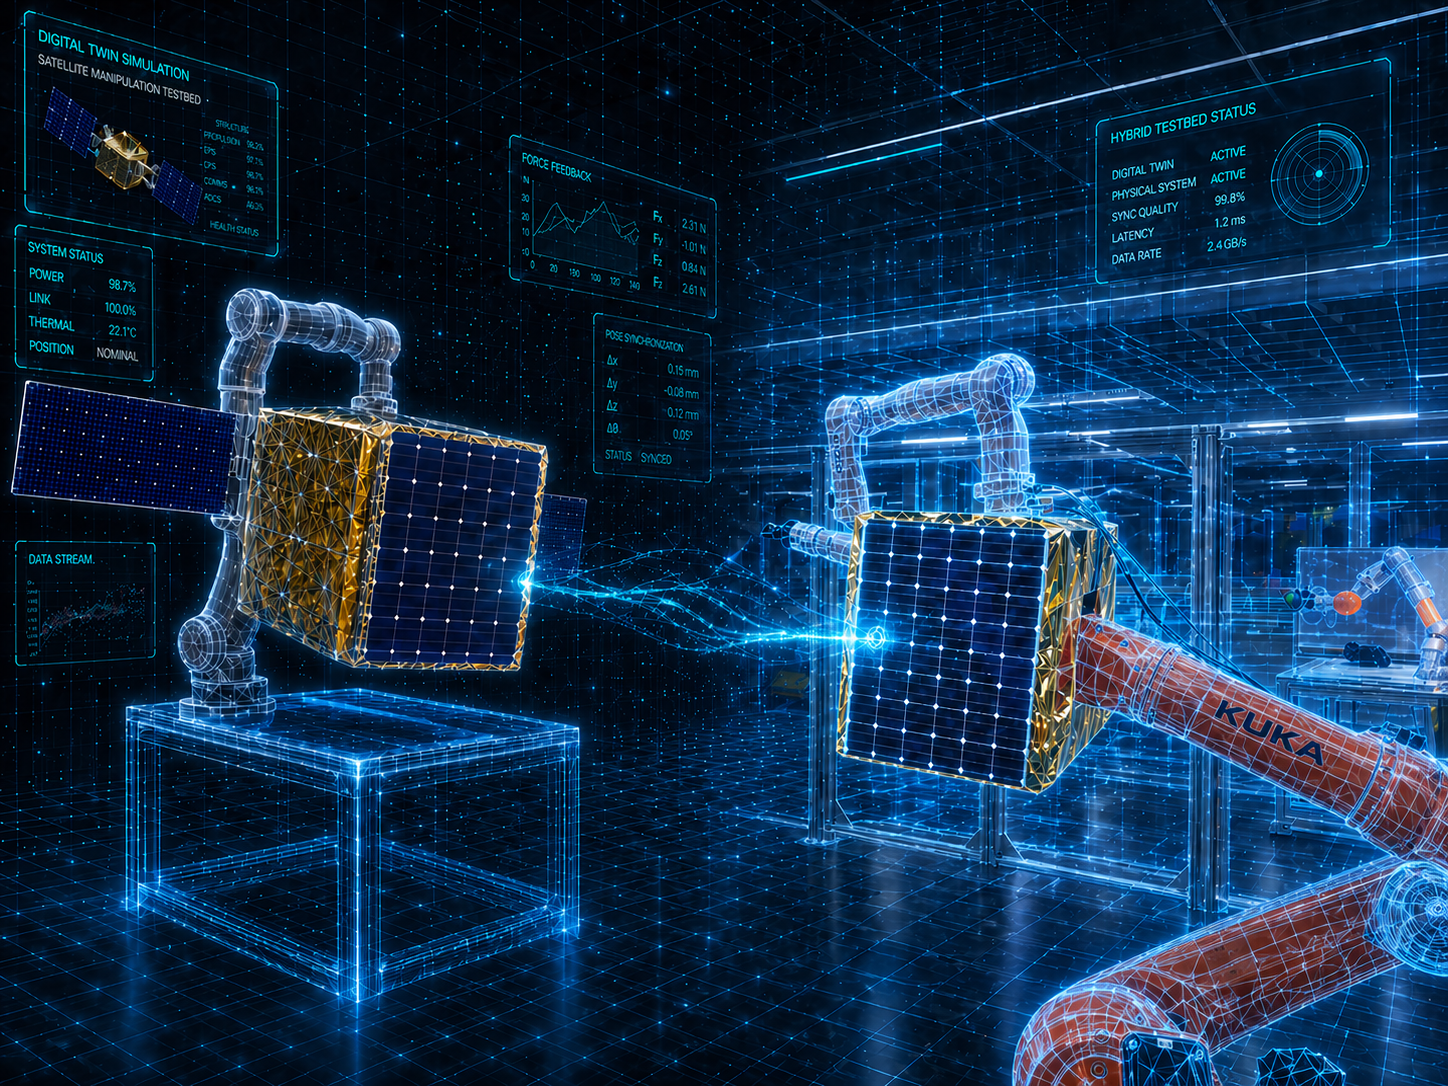
\includegraphics[width=\linewidth]{Figures/oos0.png}
	\end{subfigure}
	\caption{\DIFaddFL{Virtual testbeds based on AI-driven digital twins support the safe and repeatable
  development of learning-based control methods for in-space operations under realistic yet controllable
  conditions. Illustration created using a picture of the physical setup 
  and with the help of GPT-Image-2.}}
	\label{fig:oos0}
\end{figure}

\DIFaddend Free-floating robot manipulators operating in \DIFdelbegin \DIFdel{the space environment to inspect}\DIFdelend \DIFaddbegin \DIFadd{space for satellite inspection}\DIFaddend , capture, or \DIFdelbegin \DIFdel{de-orbit  satellites are expected to
introduce unique control challenges when compared to }\DIFdelend \DIFaddbegin \DIFadd{de-orbiting 
introduce control challenges not encountered with }\DIFaddend terrestrial robots \cite{b1}.
In micro-gravity, the robot\DIFdelbegin \DIFdel{’}\DIFdelend \DIFaddbegin \DIFadd{'}\DIFaddend s base (typically a spacecraft) is not fixed and \DIFdelbegin \DIFdel{thrusters are turned off}\DIFdelend \DIFaddbegin \DIFadd{the thrusters are inactive}\DIFaddend .
Manipulator motions \DIFdelbegin \DIFdel{can give rise to a change of }\DIFdelend \DIFaddbegin \DIFadd{therefore change }\DIFaddend the position and orientation of the base, which in turn modifies the 
\DIFdelbegin \DIFdel{final }\DIFdelend pose of the end-effector. This reaction is \DIFdelbegin \DIFdel{due to }\DIFdelend \DIFaddbegin \DIFadd{a consequence of }\DIFaddend the conservation of
\DIFdelbegin \DIFdel{the }\DIFdelend linear and angular momentum \cite{b6}. \DIFdelbegin \DIFdel{The }\DIFdelend \DIFaddbegin \DIFadd{Operating the manipulator under }\DIFaddend free-floating dynamics \DIFdelbegin \DIFdel{of space robots has many benefits. 
An expensive consumption of fuel, such as hydrazine ($N_2H_4$), and  an excitation of the robot dynamics for some activation 
frequencies of the pulse width modulation related to thruster control can be avoided }\DIFdelend \DIFaddbegin \DIFadd{avoids the 
consumption of propellant (e.g.\ hydrazine, $\mathrm{N_2H_4}$) and the excitation of structural modes by 
the pulse-width modulation of thruster control at certain frequencies }\DIFaddend \cite{b11}. This \DIFdelbegin \DIFdel{has the potential to extend the lifetime of space robots and enhance the }\DIFdelend \DIFaddbegin \DIFadd{extends the operational 
lifetime of the spacecraft and supports }\DIFaddend mission success.


However, a free-floating base complicates \DIFdelbegin \DIFdel{the achievement of robotized manipulations.
Indeed, }\DIFdelend \DIFaddbegin \DIFadd{manipulator control.
Standard motion-planning approaches developed for fixed-base robots can fail to drive }\DIFaddend the end-effector \DIFdelbegin \DIFdel{of the arm may fail to 
reach }\DIFdelend \DIFaddbegin \DIFadd{to 
}\DIFaddend the desired target\DIFdelbegin \DIFdel{point if standard motion planning approaches dedicated to robots with a 
fixed base are simply applied. Further }\DIFdelend \DIFaddbegin \DIFadd{. Additional }\DIFaddend constraints, such as communication latency
and limited onboard computational resources, \DIFdelbegin \DIFdel{make more intricate the }\DIFdelend \DIFaddbegin \DIFadd{further complicate }\DIFaddend continuous real-time control and \DIFdelbegin \DIFdel{stabilization of the base 
\mbox{%DIFAUXCMD
\cite{b1,b32}}\hskip0pt%DIFAUXCMD
. In fact, traditional control
}\DIFdelend \DIFaddbegin \DIFadd{base 
stabilization \mbox{%DIFAUXCMD
\cite{b1,b32}}\hskip0pt%DIFAUXCMD
. Model-based }\DIFaddend approaches that assume an accurate \DIFdelbegin \DIFdel{model of the robot dynamics (e.g.}\DIFdelend \DIFaddbegin \DIFadd{dynamic model (e.g.\ }\DIFaddend reactionless 
planning or precise attitude control)
\DIFdelbegin \DIFdel{can struggle to adapt to uncertainties }\DIFdelend \DIFaddbegin \DIFadd{are sensitive to model uncertainty }\DIFaddend and unmodeled dynamics. Supervised data-driven approaches \DIFdelbegin \DIFdel{, on the other hand, are }\DIFdelend \DIFaddbegin \DIFadd{are also 
}\DIFaddend difficult to apply \DIFdelbegin \DIFdel{. 
Usually, the required }\DIFdelend \DIFaddbegin \DIFadd{because
labeled training data of sufficient }\DIFaddend amount and quality \DIFdelbegin \DIFdel{of data are rather }\DIFdelend \DIFaddbegin \DIFadd{are typically }\DIFaddend unavailable in the space sector.
In \DIFdelbegin \DIFdel{many cases, robotized tracking capabilities }\DIFdelend \DIFaddbegin \DIFadd{addition, tracking capability }\DIFaddend under a free-floating \DIFdelbegin \DIFdel{behavior of the arm's base need }\DIFdelend \DIFaddbegin \DIFadd{base often has }\DIFaddend to be
demonstrated \DIFdelbegin \DIFdel{long }\DIFdelend before the physical \DIFdelbegin \DIFdel{robot }\DIFdelend system is assembled and deployed 
\cite{muhlbauer2025software,rybus2024robotic,kaigom2011optimal}.
\DIFaddbegin 


\DIFaddend These challenges motivate the development and simulation of \DIFdelbegin \DIFdel{AI-empowered digital twins 
\mbox{%DIFAUXCMD
\cite{kaigom2025deep} }\hskip0pt%DIFAUXCMD
under desired operational conditions to
explore }\DIFdelend \DIFaddbegin \DIFadd{AI-enabled digital twins 
(DTs) \mbox{%DIFAUXCMD
\cite{kaigom2025deep}}\hskip0pt%DIFAUXCMD
, as illustrated in \mbox{%DIFAUXCMD
\cref{fig:oos0}}\hskip0pt%DIFAUXCMD
. Unlike standard DTs that primarily mirror 
sensed real-time data from physical counterparts, the DTs considered here combine physics-based simulation 
with learning components to contextualize system states and evaluate representative operating conditions. 
These conditions include uncertain dynamics, disturbances, faults, and contact-rich interactions associated 
with satellite capture. Faster-than-real-time simulation and systematic ablation studies can support 
controller design and help assess sim-to-real effects. In this role, AI-enabled DTs provide a training 
and validation environment for }\DIFaddend learning-based \DIFdelbegin \DIFdel{control methods that can autonomously adapt to complex and unknown dynamicseven in the case of data scarcity}\DIFdelend \DIFaddbegin \DIFadd{controllers that combine safe exploration, policy optimization, 
and domain randomization under limited flight data and safety-critical constraints}\DIFaddend .



\begin{table*}[!t]
	\centering
	\caption{Recent advances in Deep RL-based motion management for free-floating space robots.
  \DIFaddbeginFL \DIFaddFL{Abbreviations: RL Alg.\,=\,reinforcement learning algorithm; DOF\,=\,degrees of freedom;
  Obs./Act.\,Dim.\,=\,observation-/action-space dimension; vel.\,=\,joint velocities;
  rates\,=\,joint rate commands; pos./att.\,=\,position/attitude; pos./ori.\,=\,position/orientation;
  EE\,=\,end-effector; Formal Ver.\,=\,formal verification; Base Dist.\,Min.\,=\,base disturbance minimization;
  $d_\text{safe}$\,=\,minimum admissible distance; $\tau_\text{max}$\,=\,torque bound;
  K1--K9\,=\,evaluation KPIs (see Section~\ref{RL}); N/R\,=\,not reported.}\DIFaddendFL }
	\label{tab:sample}
	\DIFdelbeginFL %DIFDELCMD < \begin{tabular}{lccc}
%DIFDELCMD < 		\toprule
%DIFDELCMD < 		\textbf{Contribution} & \textbf{RL Algorithm} & \textbf{Task Objective} & \makecell{\textbf{Formal Verification/} \\ \textbf{Base Disturbance Min.}} \\
%DIFDELCMD < 		\midrule
%DIFDELCMD < 		\cite{huang2023obstacle}, 2023 & SAC & Obstacle avoidance & No/No \\
%DIFDELCMD < 		\cite{al2024reinforcement}, 2024 & DDPG & Collision avoidance & No/No \\
%DIFDELCMD < 		\cite{d2024failure}, 2024 & PPO & Adaptation to joint failure & No/No \\
%DIFDELCMD < 		\cite{al2024path}, 2024 & DDPG & Path planning & No/No \\
%DIFDELCMD < 		\cite{hu2025deep}, 2025 & PPO & Trajectory planning & No/No \\
%DIFDELCMD < 		\cite{zhang2025learning}, 2025 & LSAC & Trajectory post-processing & No/No \\
%DIFDELCMD < 		\cite{wei2025trajectory}, 2025 & DDPG & Trajectory planning & No/Yes \\
%DIFDELCMD < 		\bottomrule
%DIFDELCMD < 	\end{tabular}
%DIFDELCMD < %%%
\DIFdelendFL \DIFaddbeginFL \scriptsize
	\renewcommand{\arraystretch}{1.25}
	\begin{tabular}{lcccccccc}
		\toprule
		\textbf{Contribution} & \makecell{\textbf{RL}\\\textbf{Alg.}} & \textbf{Task Objective} & \textbf{DOF} & \textbf{Simulator} & \makecell{\textbf{Obs./Act.}\\\textbf{Dim.}} & \makecell{\textbf{Safety}\\\textbf{Limits}} & \makecell{\textbf{Eval.}\\\textbf{Metrics}} & \makecell{\textbf{Formal Ver./}\\\textbf{Base Dist. Min.}} \\
		\midrule
		\cite{huang2023obstacle}, 2023 & SAC & Obstacle avoidance & 7 & OpenAI Gym & 14\,/\,7D vel. & Reward-based & Success rate & No/No \\
		\cite{al2024reinforcement}, 2024 & DDPG & Collision avoidance & 6 & Custom & N/R\,/\,6D vel. & Reward-based & Success rate & No/No \\
		\cite{d2024failure}, 2024 & PPO & \makecell{Joint failure\\adaptation} & 7 & \makecell{MATLAB\\Simscape + SPART} & 32\,/\,7D rates & \makecell{Pos./att.\\threshold} & \makecell{Per-joint\\success rate} & No/No \\
		\cite{al2024path}, 2024 & DDPG & Path planning & 6 & Custom & 32\,/\,6D vel. & Reward-based & \makecell{Convergence,\\task completion} & No/No \\
		\cite{hu2025deep}, 2025 & PPO & Trajectory planning & 6 & PyBullet & N/R\,/\,6D & Joint limits & \makecell{Success rate,\\pos./ori. error} & No/No \\
		\cite{zhang2025learning}, 2025 & LSAC & \makecell{Trajectory\\post-processing} & N/R & \makecell{Custom +\\air-bearing} & N/R\,/\,N/R & \makecell{Uncertainty\\bounds} & Tracking error & No/No \\
		\cite{wei2025trajectory}, 2025 & DDPG & Trajectory planning & N/R & Custom & N/R\,/\,N/R & \makecell{Base dist.\\(soft)} & \makecell{Reward,\\base dist. red.} & No/Yes \\
		\midrule
		\textbf{Ours} & \textbf{PPO} & \makecell{\textbf{Cartesian EE}\\\textbf{tracking}} & \textbf{4} & \makecell{\textbf{MATLAB/Simulink}\\\textbf{+ Simscape}} & \textbf{23\,/\,4D} $\boldsymbol{\tau}$ & \makecell{$d_\text{safe}$, $\tau_\text{max}$,\\joint limits} & K1--K9 & \textbf{Yes/Yes} \\
		\bottomrule
	\end{tabular}
\DIFaddendFL \end{table*}

Reinforcement \DIFdelbegin \DIFdel{Learning }\DIFdelend \DIFaddbegin \DIFadd{learning }\DIFaddend (RL) has \DIFdelbegin \DIFdel{emerged as a promising approach for }\DIFdelend \DIFaddbegin \DIFadd{been increasingly applied in }\DIFaddend robotics, enabling agents to
\DIFdelbegin \DIFdel{learn }\DIFdelend \DIFaddbegin \DIFadd{synthesize }\DIFaddend control policies through trial-and-error \DIFdelbegin \DIFdel{interactions with entities, environments, and processes}\DIFdelend \DIFaddbegin \DIFadd{interaction with their environment}\DIFaddend . Recent advances in deep RL have \DIFdelbegin \DIFdel{shown
success in complex control tasks, but applying RL }\DIFdelend \DIFaddbegin \DIFadd{addressed a range of complex continuous-control tasks, although applications }\DIFaddend to space robots \DIFdelbegin \DIFdel{is still relatively novel }\DIFdelend \DIFaddbegin \DIFadd{remain comparatively recent }\DIFaddend \cite{wu2020reinforcement,al2024path,hu2025deep,zhang2025learning,huang2023obstacle}.

\DIFdelbegin \DIFdel{The work presented in this paper investigates the use of }\DIFdelend \DIFaddbegin \DIFadd{This paper investigates }\DIFaddend continuous-action deep RL for \DIFdelbegin \DIFdel{the tracking of a Cartesian motion of }\DIFdelend \DIFaddbegin \DIFadd{Cartesian path tracking of }\DIFaddend the end-effector of a free-floating space
manipulator. \DIFdelbegin \DIFdel{It  differs from previous contributions in three ways}\DIFdelend \DIFaddbegin \DIFadd{The contribution differs from prior work in three respects}\DIFaddend . First, \DIFdelbegin \DIFdel{it focuses on a systematic comparison 
and explores the respective performance of }\DIFdelend six different RL algorithms \DIFdelbegin \DIFdel{beyond those mentioned e.g. in \mbox{%DIFAUXCMD
\Cref{tab:sample}}\hskip0pt%DIFAUXCMD
, thereby 
quantitatively and qualitatively contributing to filling in a current gap in space robotics}\DIFdelend \DIFaddbegin \DIFadd{are systematically compared (see \mbox{%DIFAUXCMD
\cref{comparison}}\hskip0pt%DIFAUXCMD
) and complemented by ablation studies (see \mbox{%DIFAUXCMD
\cref{sec:reward_ablation}}\hskip0pt%DIFAUXCMD
), addressing a gap left by the works listed in \mbox{%DIFAUXCMD
\Cref{tab:sample}}\hskip0pt%DIFAUXCMD
}\DIFaddend . Second, \DIFdelbegin \DIFdel{several constraints , }\DIFdelend \DIFaddbegin \DIFadd{constraints }\DIFaddend such as collision avoidance \DIFdelbegin \DIFdel{, }\DIFdelend are monitored
through formal methods \DIFdelbegin \DIFdel{applied from a software-enabled and practical perspective. Finally, this work investigates the minimization of the 
base attitude }\DIFdelend \DIFaddbegin \DIFadd{integrated into the simulation toolchain (see \mbox{%DIFAUXCMD
\cref{formal}}\hskip0pt%DIFAUXCMD
). Third, base attitude minimization during arm motion is treated as an explicit control objective }\DIFaddend in conjunction with \DIFdelbegin \DIFdel{constraint monitoring previously mentioned. Recall that the }\DIFdelend \DIFaddbegin \DIFadd{the constraint monitoring above. The }\DIFaddend induced base disturbance is \DIFdelbegin \DIFdel{omitted in most recent contributions, 
as highlighted }\DIFdelend \DIFaddbegin \DIFadd{not addressed in most of the works listed }\DIFaddend in \Cref{tab:sample}. \DIFdelbegin \DIFdel{We are not aware of any comprehensive work that compares  }\DIFdelend \DIFaddbegin \DIFadd{To the authors' knowledge, a unified comparison of }\DIFaddend RL algorithms
for \DIFdelbegin \DIFdel{the }\DIFdelend Cartesian path tracking of free-floating space robots \DIFdelbegin \DIFdel{while considering the }\DIFdelend \DIFaddbegin \DIFadd{that jointly considers }\DIFaddend base attitude minimization and \DIFdelbegin \DIFdel{unifying 
constraint monitoring by leveraging formal methods, to the best of our knowledge (see, also }%DIFDELCMD < \autoref{tab:sample}%%%
\DIFdel{)}\DIFdelend \DIFaddbegin \DIFadd{formal-methods-based constraint monitoring remains unavailable.
}

\DIFadd{As shown in }\autoref{tab:sample}\DIFadd{, the surveyed prior contributions typically evaluate a single RL algorithm on a specific subtask, which limits conclusions about the relative merits of different learning paradigms for free-floating space robot control. Furthermore, the surveyed literature does not jointly address three compounding challenges: (i)~a multi-algorithm benchmark under strictly unified conditions, (ii)~explicit minimization of base attitude disturbance as a co-equal control objective alongside end-effector tracking, and (iii)~integration of formal safety verification directly into the RL training loop. The present work addresses these gaps jointly by providing a reproducible and safety-aware comparison framework that extends the individual studies listed in }\autoref{tab:sample}\DIFaddend .

The \DIFdelbegin \DIFdel{key 
contributions and novelties }\DIFdelend \DIFaddbegin \DIFadd{main contributions }\DIFaddend of this work \DIFdelbegin \DIFdel{include}\DIFdelend \DIFaddbegin \DIFadd{are summarized as follows}\DIFaddend :

\begin{itemize}
  \item \DIFdelbegin \DIFdel{A comparative evaluation of RL Agents: We implement and evaluate six state-of-the-art
continuous RL algorithms , }\DIFdelend \DIFaddbegin \textit{\DIFadd{Comparative evaluation of RL agents.}} \DIFadd{Six continuous-action RL algorithms are implemented and evaluated on the same path-tracking task. The algorithms are }\DIFaddend Trust Region Policy Optimization (TRPO) \cite{b14}, Twin Delayed Deep
Deterministic Policy Gradient (TD3) \cite{b17}, Soft Actor-Critic (SAC) \cite{b18}, Proximal Policy Optimization
(PPO) \cite{b15}, vanilla Policy Gradient (PG) \cite{b21}, and Deep Deterministic Policy Gradient (DDPG) \cite{b7}\DIFdelbegin \DIFdel{, on the same path tracking task of a free-floating robot. This side-by-side comparison }\DIFdelend \DIFaddbegin \DIFadd{. The comparison is performed }\DIFaddend under unified conditions \DIFdelbegin \DIFdel{reveals which algorithm is likely to deliver the best possible performance when it comes to motion tracking of a free-floating space robot and why}\DIFdelend \DIFaddbegin \DIFadd{and identifies which algorithm offers the most favorable trade-off between tracking accuracy, base disturbance, and training stability}\DIFaddend .
  \item \DIFdelbegin \DIFdel{An integration of formal safety measures: To meet safety-critical space operation requirements,
we incorporate formal methods }\DIFdelend \DIFaddbegin \textit{\DIFadd{Integration of formal safety mechanisms.}} \DIFadd{Formal methods are integrated }\DIFaddend into the learning loop \cite{b5, b6, b22, b23}. A collision \DIFdelbegin \DIFdel{monitoring, momentum
conservation check , and formal verification of joint torque limits are embedded in the simulation. This integration 
ensures the RL agent cannot violate fundamental and critical }\DIFdelend \DIFaddbegin \DIFadd{monitor and a momentum-conservation check run at runtime, and the joint-torque bound is additionally verified offline with a model checker on a bounded abstraction of the policy. This combination monitors the targeted }\DIFaddend safety properties (\DIFdelbegin \DIFdel{like avoiding collisions or exceeding actuator limits}\DIFdelend \DIFaddbegin \DIFadd{collision avoidance and bounded actuator commands}\DIFaddend ) during training and testing.
 \item \DIFdelbegin \DIFdel{A high-fidelity simulation environment: We develop a high-fidelity }\DIFdelend \DIFaddbegin \textit{\DIFadd{Simulation environment for multi-criteria evaluation in on-orbit servicing.}} \DIFadd{A }\DIFaddend MATLAB/Simulink simulation \DIFdelbegin \DIFdel{of }\DIFdelend \DIFaddbegin \DIFadd{framework is developed for }\DIFaddend a free-floating space robot \DIFdelbegin \DIFdel{, using a URDF-based }\DIFdelend \DIFaddbegin \DIFadd{based on a URDF-derived }\DIFaddend multibody model and the Simscape physics engine. The robot \DIFdelbegin \DIFdel{, a cube-shaped base with a 4-Degree of Freedom (DOF) robotic arm, is modeled with realistic kinematics, dynamics}\DIFdelend \DIFaddbegin \DIFadd{consists of a cuboid base and a 4-degree-of-freedom (4-DOF) revolute arm, modeled with consistent kinematic, inertial}\DIFaddend , and sensor/actuator parameters\DIFdelbegin \DIFdel{and features. A dedicated reinforcement learning environment provides the agent with }\DIFdelend \DIFaddbegin \DIFadd{. The associated RL environment provides }\DIFaddend observations and rewards \DIFdelbegin \DIFdel{, including 
a specially designed }\DIFdelend \DIFaddbegin \DIFadd{through a composite }\DIFaddend reward function that \DIFdelbegin \DIFdel{encourages accurate }\DIFdelend \DIFaddbegin \DIFadd{penalizes }\DIFaddend end-effector \DIFdelbegin \DIFdel{trajectory tracking while penalizing base movement}\DIFdelend \DIFaddbegin \DIFadd{tracking error, base motion}\DIFaddend , large joint velocities, and excessive control effort\DIFdelbegin \DIFdel{(energy). Through reward shaping and carefully chosen }\DIFdelend \DIFaddbegin \DIFadd{. Together with the }\DIFaddend reset conditions, \DIFdelbegin \DIFdel{the agent learns to accomplish the task without causing 
excessive base disturbance or safety violations }\DIFdelend \DIFaddbegin \DIFadd{this reward shaping allows the agent to learn the task while keeping base disturbance and safety violations bounded }\DIFaddend \cite{b25,b26,b27,b28,b7}.
 \item \DIFdelbegin \DIFdel{The optimization of the PPO agent : }\DIFdelend \DIFaddbegin \textit{\DIFadd{Optimization of the PPO agent.}} \DIFaddend Based on the comparative results, \DIFdelbegin \DIFdel{we identify PPO as the top-
performing algorithm and further refine it for path tracking tasks. We adjust the }\DIFdelend \DIFaddbegin \DIFadd{PPO is selected for further tuning. The }\DIFaddend neural network architecture and \DIFdelbegin \DIFdel{tune hyperparameters (e.g., }\DIFdelend \DIFaddbegin \DIFadd{key hyperparameters (}\DIFaddend learning rate, \DIFaddbegin \DIFadd{mini-}\DIFaddend batch size, clipping ratio, \DIFdelbegin \DIFdel{entropy
regularization, etc.) }\DIFdelend \DIFaddbegin \DIFadd{and entropy regularization) are adjusted }\DIFaddend to improve training stability and policy performance. The optimized PPO agent \DIFdelbegin \DIFdel{achieves significantly better tracking accuracy, }\DIFdelend \DIFaddbegin \DIFadd{reduces tracking error, produces }\DIFaddend smoother control inputs, and \DIFdelbegin \DIFdel{zero
safety violations , outperforming the }\DIFdelend \DIFaddbegin \DIFadd{shows no safety violations in the reported evaluation episodes relative to the }\DIFaddend default configuration on \DIFdelbegin \DIFdel{all key metrics}\DIFdelend \DIFaddbegin \DIFadd{the tested KPIs}\DIFaddend .
\end{itemize}
%DIF < \newpage
\DIFdelbegin \DIFdel{Overall, our study shows that a combination of multiple-body }\DIFdelend \DIFaddbegin 

\DIFadd{The integration of multibody }\DIFaddend simulation, deep \DIFdelbegin \DIFdel{RL}\DIFdelend \DIFaddbegin \DIFadd{reinforcement learning}\DIFaddend , and formal verification \DIFdelbegin \DIFdel{can yield a robust and safe control policy for a free-floating space robot. In the following, we first describe the system modeling and RL framework, then detail the formal safety components, present a comparative analysis of the RL agents, and finally discuss the optimized PPO agent ’s performance, before concluding with broader insights and future directions}\DIFdelend \DIFaddbegin \DIFadd{considered here yields control policies that respect the imposed safety constraints while reducing tracking error and base disturbance relative to the default configuration. The remainder of the paper is organized as follows. Section~\ref{sec:sim} describes the system model and the simulation environment. Section~\ref{RL} introduces the reinforcement learning framework. Section~\ref{formal} presents the safety monitors and formal-methods components. Section~\ref{comparison} reports the comparative evaluation of the six RL algorithms. The optimization of the PPO agent and its evaluation on circular and piecewise-linear references follow, before discussion and conclusion}\DIFaddend .

\section{Related Work}
\DIFaddbegin 

\DIFaddend \subsection{\DIFdelbegin \DIFdel{Reinforcement Learning for Robotic }\DIFdelend \DIFaddbegin \DIFadd{Classical }\DIFaddend Control \DIFaddbegin \DIFadd{Techniques for Space Robots}\DIFaddend }
\DIFaddbegin \DIFadd{Model-based approaches have historically dominated space robot control. Computed torque control and resolved-motion rate methods leverage accurate dynamic models to achieve precise end-effector positioning \mbox{%DIFAUXCMD
\cite{b1}}\hskip0pt%DIFAUXCMD
. Reactionless path planning explicitly
minimizes base disturbance by exploiting the robot's redundancy and a dynamics-related null-space to design joint velocities, while attitude regulation methods use reaction wheels or thrusters
to counteract momentum transfer \mbox{%DIFAUXCMD
\cite{b6,kaigom2011optimal}}\hskip0pt%DIFAUXCMD
. These approaches offer strong performance guarantees and
interpretability when the system model is accurate. However, they are sensitive to model uncertainties and unmodeled
dynamics, require significant engineering effort for model identification, and are ill-suited to the data-scarce,
hazardous conditions of on-orbit operations.
}

\subsection{\DIFadd{Reinforcement Learning-Based Control Techniques}}
\DIFaddend RL has demonstrated success in various robotic manipulation tasks \cite{b2,b7}.
Policy gradient methods (PG, PPO, TRPO) and actor-critic algorithms (DDPG, TD3, SAC)
have been widely applied to continuous control problems \cite{b14,b15,b17,b18,b21}.
\DIFdelbegin %DIFDELCMD < 

%DIFDELCMD < %%%
\subsection{\DIFdel{Control of Free-Floating Space Robots}}
%DIFAUXCMD
\addtocounter{subsection}{-1}%DIFAUXCMD
\DIFdel{Traditional approaches for space robot control include computed torque control, reactionless path planning, and attitude regulation \mbox{%DIFAUXCMD
\cite{b1,b6}}\hskip0pt%DIFAUXCMD
. Recent works 
have started exploring RL }\DIFdelend \DIFaddbegin \DIFadd{Applied to free-floating space robots, RL-based methods have been investigated }\DIFaddend for path planning \cite{wu2020reinforcement,al2024path},
obstacle avoidance \cite{huang2023obstacle}, \DIFdelbegin \DIFdel{and }\DIFdelend trajectory tracking \cite{hu2025deep}\DIFdelbegin \DIFdel{.
}\DIFdelend \DIFaddbegin \DIFadd{, and failure management \mbox{%DIFAUXCMD
\cite{d2024failure}}\hskip0pt%DIFAUXCMD
.
RL does not require an explicit dynamic model of the system, which is relevant when model parameters are uncertain or unavailable. However, current RL-based approaches share recurring limitations. Most studies
evaluate only a single algorithm, address a single objective, omit base attitude minimization, and do not provide systematic benchmarking under comparable conditions.
}\DIFaddend 

\subsection{\DIFdelbegin \DIFdel{Safe Reinforcement Learning}\DIFdelend \DIFaddbegin \DIFadd{Hybrid Safety-Aware Control Systems}\DIFaddend }
Safe RL integrates safety constraints through formal verification,
barrier functions, and constrained optimization \cite{b22,b23,b24,b34}.
\DIFdelbegin \DIFdel{However, application to space robotics with formal safety guarantees remains limited}\DIFdelend \DIFaddbegin \DIFadd{Shielding approaches \mbox{%DIFAUXCMD
\cite{b23} }\hskip0pt%DIFAUXCMD
intercept unsafe actions at runtime and substitute corrective commands,
while control barrier functions (CBFs) \mbox{%DIFAUXCMD
\cite{b34} }\hskip0pt%DIFAUXCMD
encode safety as a continuously enforced constraint on the policy's action set.
These hybrid methods combine the adaptability of RL with formally specified runtime constraints, helping to enforce critical properties such as joint limit compliance
and collision avoidance. However, their application to free-floating space robots remains largely unexplored:
existing works rarely integrate formal verification directly into the RL training loop or combine it with base attitude minimization objectives}\DIFaddend .

\subsection{\DIFdelbegin \DIFdel{Research Gap}\DIFdelend \DIFaddbegin \DIFadd{Need for Benchmark Studies}\DIFaddend }
\DIFdelbegin \DIFdel{Despite recent advances, systematic comparisons }\DIFdelend \DIFaddbegin \DIFadd{Comparative evaluations }\DIFaddend of RL algorithms for \DIFdelbegin \DIFdel{free-floating 
}\DIFdelend space robot control are \DIFdelbegin \DIFdel{lacking. Most prior works focus on single algorithms and omit base attitude minimizationor }\DIFdelend \DIFaddbegin \DIFadd{scarce. Table~\ref{tab:sample} surveys recent deep RL
contributions to free-floating space robot motion management. As shown, all surveyed works address only individual
goals with a single algorithm. None simultaneously combines multi-algorithm and multi-criteria benchmarking, base disturbance minimization,
and }\DIFaddend formal safety verification\DIFaddbegin \DIFadd{. This absence of unified evaluation makes it difficult to draw conclusions about relative
algorithm performance and to guide algorithm selection for future missions.
}

\subsection{\DIFadd{Research Gap}}
\DIFadd{The preceding survey reveals three mutually reinforcing gaps in the existing literature. First, no prior work systematically compares multiple RL algorithms under identical conditions for Cartesian end-effector tracking of free-floating space robots. Second, base attitude minimization, a safety-critical requirement in on-orbit operations, is omitted in most RL-based
contributions }\DIFaddend (see Table~\ref{tab:sample}). \DIFaddbegin \DIFadd{Third, the integration of formal safety verification directly into the RL
training and evaluation loop has not been demonstrated for this class of systems. The present work addresses all
three gaps simultaneously. It benchmarks six representative RL algorithms under unified conditions, incorporates base
attitude minimization as an explicit control objective, and integrates formal safety monitoring into the RL training and
evaluation loop, with the actuator-torque bound additionally established by offline model checking.
}\DIFaddend 

\section{System Modeling and Simulation Environment}\DIFaddbegin \label{sec:sim}
\DIFaddend \begin{figure*}[!t]
    \centering
  \DIFdelbeginFL %DIFDELCMD < \begin{subfigure}{0.48\textwidth}
%DIFDELCMD <         %%%
\DIFdelendFL %DIF >   \begin{subfigure}{0.48\textwidth}
  %DIF >       \centering
  %DIF >       %
\includegraphics[width=\linewidth]{Figures/ref_kreisbahn_1.png%}
   %DIF >  \end{subfigure}
 %DIF >    \hfill
    \DIFaddbeginFL \begin{subfigure}{0.45\textwidth}
        \DIFaddendFL \centering
        \DIFdelbeginFL %DIFDELCMD < 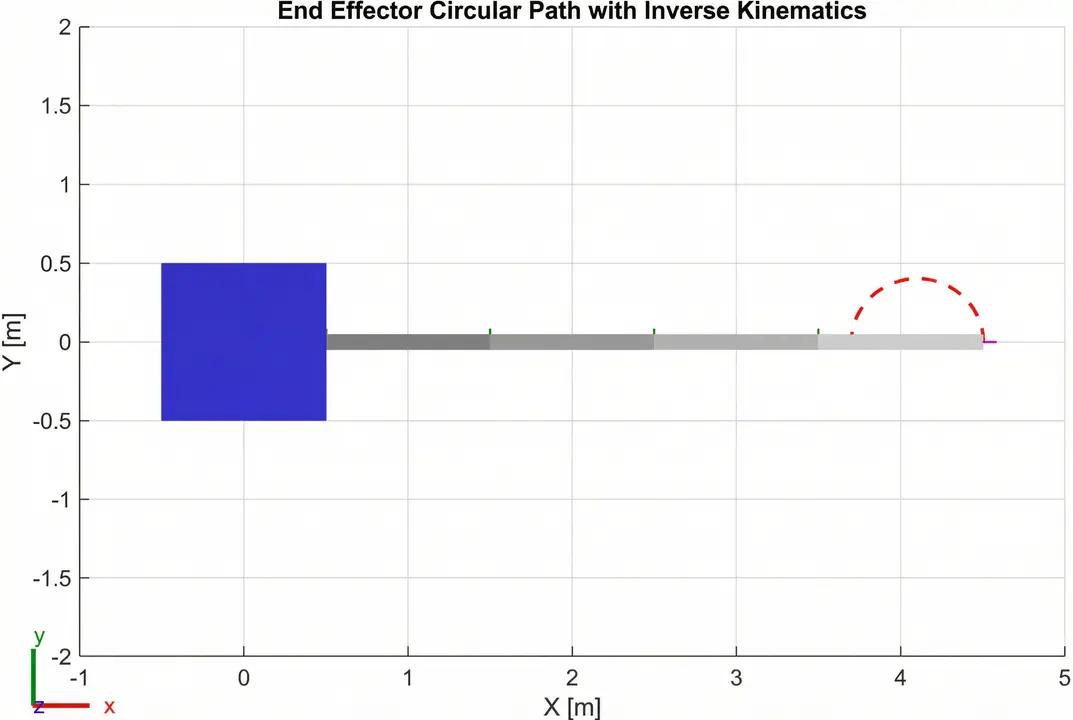
\includegraphics[width=\linewidth]{Figures/ref_kreisbahn_1.png}
%DIFDELCMD <     \end{subfigure}
%DIFDELCMD <     \hfill
%DIFDELCMD <     \begin{subfigure}{0.48\textwidth}
%DIFDELCMD <         \centering
%DIFDELCMD <         %%%
\DIFdelendFL 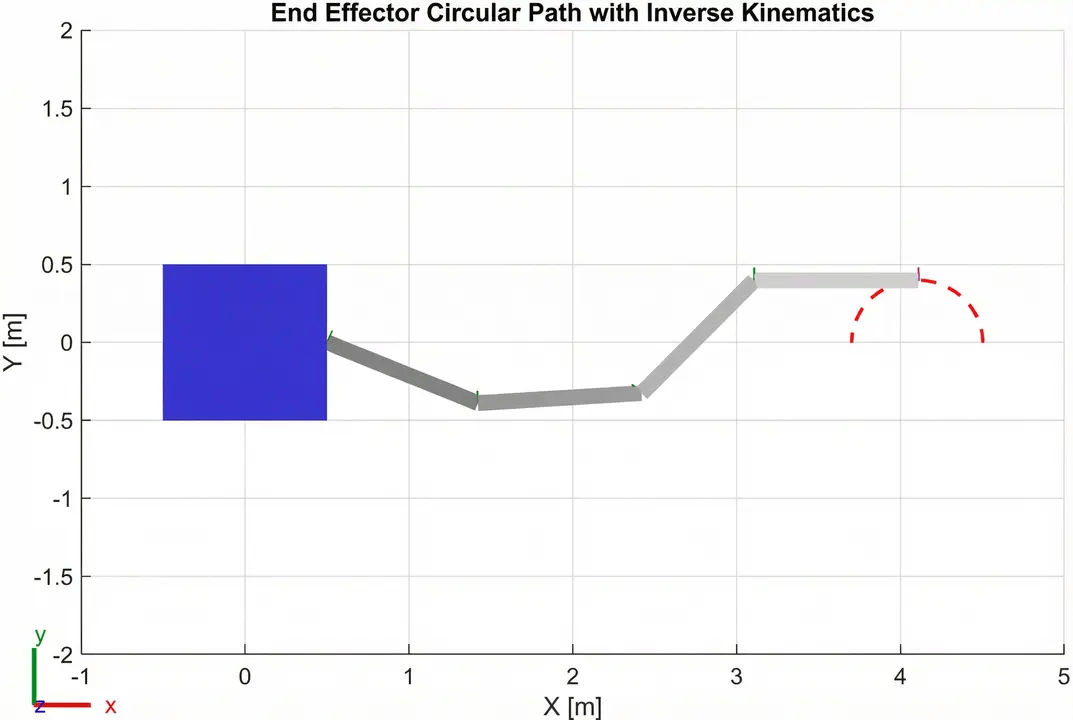
\includegraphics[width=\linewidth]{Figures/ref_kreisbahn_2.png}
    \end{subfigure}
    \DIFdelbeginFL %DIFDELCMD < 

%DIFDELCMD <     %%%
\DIFdelendFL \vspace{0.5em}
    \DIFdelbeginFL %DIFDELCMD < \begin{subfigure}{0.5\textwidth}
%DIFDELCMD <         %%%
\DIFdelendFL \DIFaddbeginFL \begin{subfigure}{0.45\textwidth}
        \DIFaddendFL \centering
        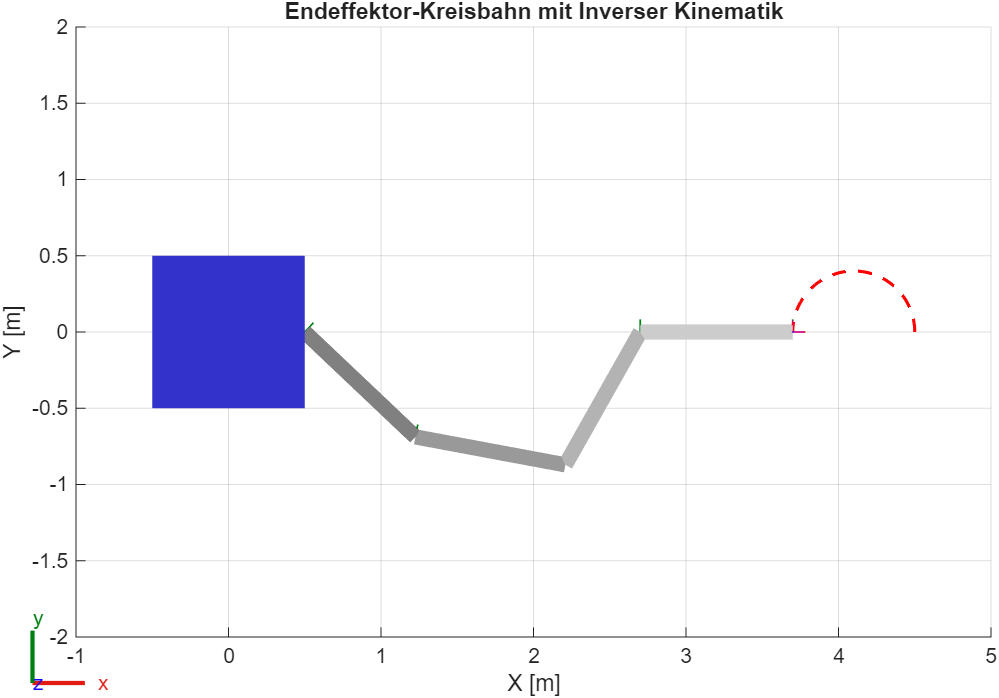
\includegraphics[width=\linewidth]{Figures/ref_kreisbahn_3.png}
    \end{subfigure}
    \caption{Tracking the desired end-effector circular path using inverse kinematics.}
    \label{fig:ref_kreis_gesamt}
\end{figure*}
\noindent
\subsection{Advantages of AI-Endowed Digital Twin Technology in On-Orbit Servicing}
\DIFaddbegin 

\DIFaddend Recent advances in AI-driven \DIFdelbegin \DIFdel{digital twinning }\DIFdelend \DIFaddbegin \DIFadd{DTs }\DIFaddend have demonstrated considerable benefits for on-orbit servicing, ranging from automated lifecycle management of satellites to the orchestration of skillful agents that autonomously carry out complex assembly, integration, and testing tasks \cite{leutert2024ai,muhlbauer2025towards}. By combining contextualized real-time sensor data with AI \DIFdelbegin \DIFdel{that accommodates 
uncertainties, digital twins }\DIFdelend \DIFaddbegin \DIFadd{methods that account for uncertainty, DTs }\DIFaddend bridge the physical and digital \DIFdelbegin \DIFdel{world with accelerated }\DIFdelend \DIFaddbegin \DIFadd{domains and enable }\DIFaddend simulation-driven analysis under \DIFdelbegin \DIFdel{desired operational conditions and at low costs}\DIFdelend \DIFaddbegin \DIFadd{diverse operational conditions at reduced cost}\DIFaddend . Verification and validation also benefit from this paradigm, as changes in system design or operational scenarios can be described in scenario spaces and integrated with \DIFdelbegin \DIFdel{digital twins }\DIFdelend \DIFaddbegin \DIFadd{DTs }\DIFaddend for flexible verification \cite{maqbool2025systems}.

\DIFaddbegin \DIFadd{In this work,  the information model of the DTs associated with the target satellite and the chaser space robot provides a structured and interoperable description of the satellite and robotic systems, including their kinematics, inertial properties, joint configurations, and physical constraints. The AI capability is embodied by a deep reinforcement learning agent, specifically PPO, which is trained and evaluated through interaction with the corresponding DTs and additional DTs involved in representative in-space operation scenarios. This distinguishes the proposed approach from classical simulation. Rather than relying on pre-specified controllers, the robotics-related DT hosts a learning-based agent that autonomously synthesizes control strategies from experience. In this way, the DTs are not limited to reproducing predefined system behavior, but serve as adaptive training and validation environments that support the evolution of control strategies under varying operational conditions. During training, scenarios and constraints are sampled from bounded uniform distributions, allowing the agent to explore a broad range of admissible operating conditions. This improves robustness to modeling errors, disturbances, and partially unknown dynamics without requiring explicit model knowledge.
}



\DIFaddend \begin{figure*}[!t]
	\centering
	\DIFdelbeginFL %DIFDELCMD < 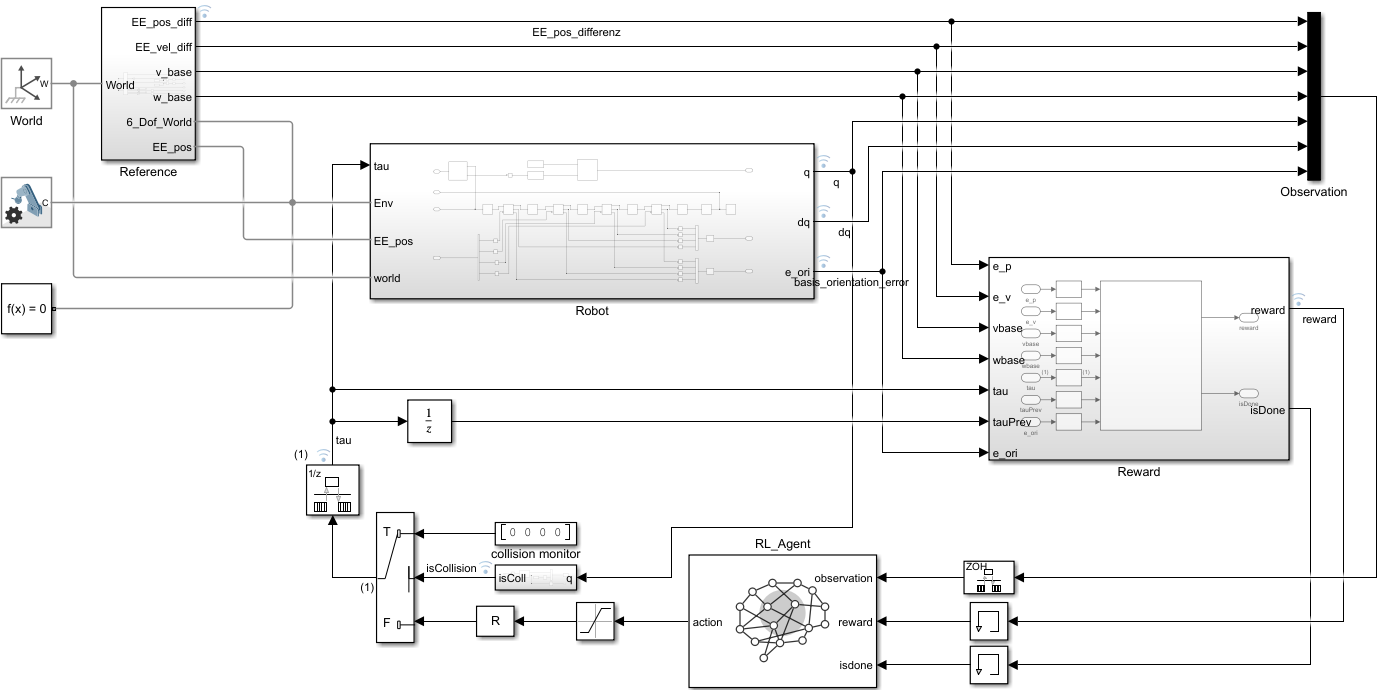
\includegraphics[width=0.98\linewidth]{Figures/Spacerobot_slx.png}
%DIFDELCMD < 	%%%
\DIFdelendFL \DIFaddbeginFL 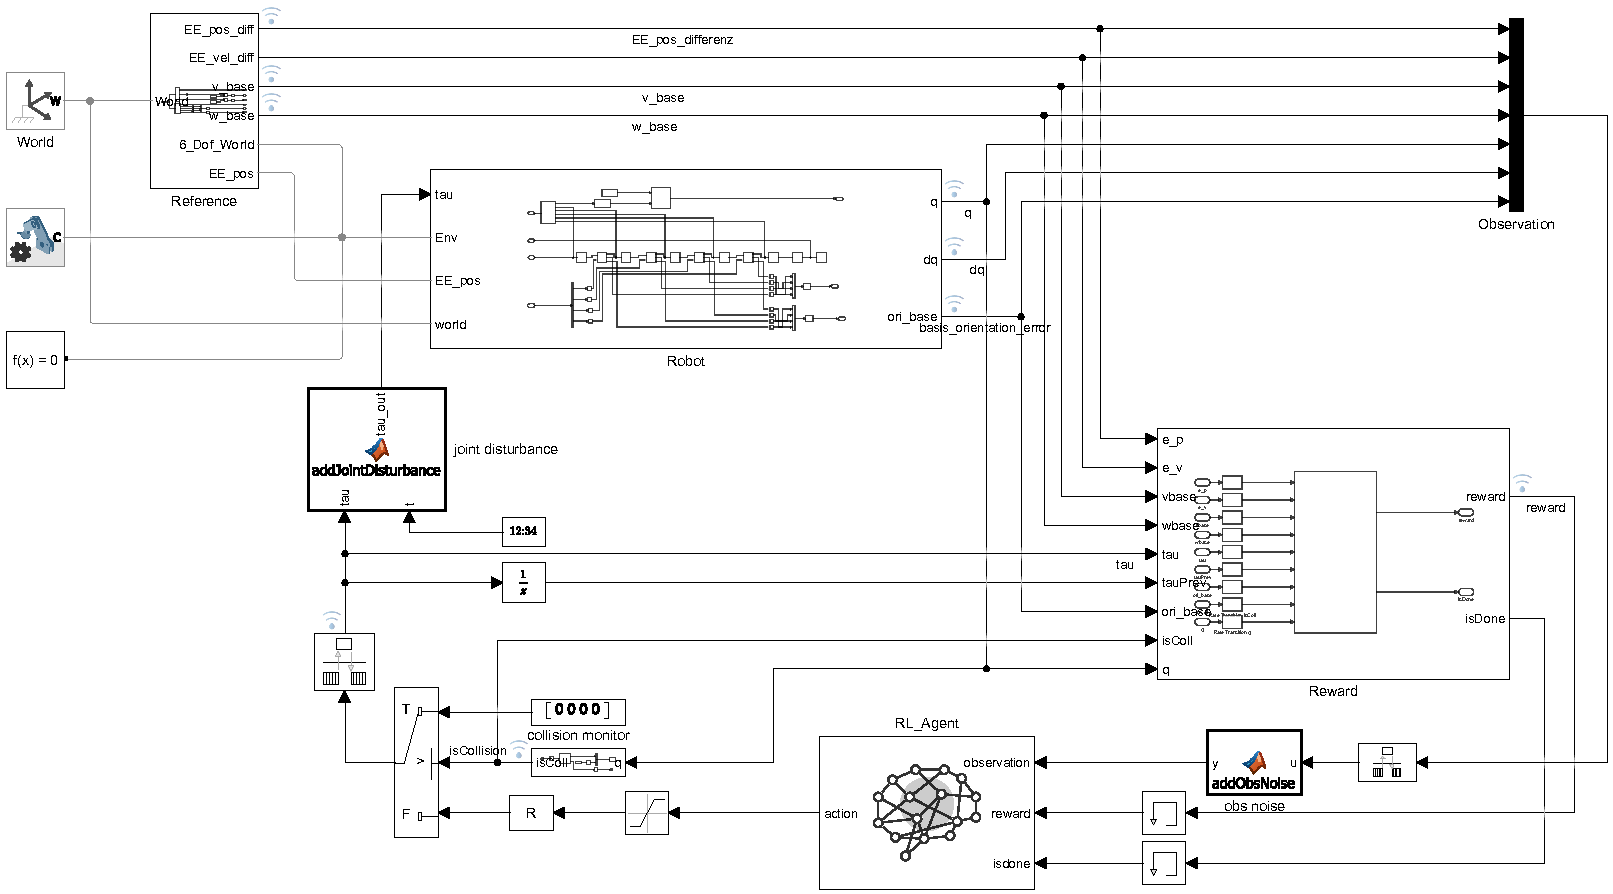
\includegraphics[width=0.98\linewidth]{Figures/Spacerobot_slx.pdf}
	\DIFaddendFL \caption{Overview of the Simulink model \texttt{SpaceRobot.slx} \\
  This figure shows the Simulink-based closed-loop simulation framework for the free-floating space robot. The model integrates the robot dynamics, 
  reference generation, observation assembly, reward computation, and a PPO-based reinforcement learning agent that outputs joint torques. The reward and 
  termination logic evaluate end-effector tracking performance, base motion disturbance, and control effort to guide policy learning.}
	\label{fig:spacerobot_slx}
\end{figure*}

\subsection{Robot Model} The virtual testbed \DIFdelbegin \DIFdel{for this research allows for the simulation of }\DIFdelend \DIFaddbegin \DIFadd{simulates }\DIFaddend a free-floating space manipulator \DIFdelbegin \DIFdel{inspired by
}\DIFdelend \DIFaddbegin \DIFadd{derived from
}\DIFaddend the Spacecraft Robotics Toolkit (SPART) example \cite{b9}. The robot consists of a cuboid base (serving as the
spacecraft) \DIFdelbegin \DIFdel{with }\DIFdelend \DIFaddbegin \DIFadd{and }\DIFaddend a 4-degree-of-freedom (4-DOF) serial manipulator \DIFdelbegin \DIFdel{arm mounted on it }\DIFdelend (see~\autoref{fig:ref_kreis_gesamt}). The arm
has four revolute joints and four links\DIFdelbegin \DIFdel{, and its }\DIFdelend \DIFaddbegin \DIFadd{. Its }\DIFaddend kinematic structure and inertial properties are \DIFdelbegin \DIFdel{defined }\DIFdelend \DIFaddbegin \DIFadd{specified }\DIFaddend in
a Unified Robot Description Format (URDF) file (\DIFdelbegin \DIFdel{SpaceRobot.urdf) which is }\DIFdelend \DIFaddbegin \texttt{\DIFadd{SpaceRobot.urdf}}\DIFadd{) }\DIFaddend imported into Simulink\DIFdelbegin \DIFdel{’s
multibody simulation }\DIFdelend \DIFaddbegin \DIFadd{'s
multibody }\DIFaddend environment \cite{b25,b26,b27}. \DIFdelbegin \DIFdel{Identified values }\DIFdelend \DIFaddbegin \DIFadd{The geometry and the inertial properties of the links are taken from identified values reported in the literature }\DIFaddend (see, \DIFdelbegin \DIFdel{.}\DIFdelend e.g., \cite{b12}) \DIFdelbegin \DIFdel{were chosen for the geometry 
and the inertial properties of links of the space arm considered in this work and }\DIFdelend \DIFaddbegin \DIFadd{and }\DIFaddend stored in the URDF model. The \DIFdelbegin \DIFdel{result is a realistic
multibody model with a floating base and an arm, capturing the strong }\DIFdelend \DIFaddbegin \DIFadd{resulting multibody model captures the }\DIFaddend dynamic coupling between \DIFdelbegin \DIFdel{them }\DIFdelend \DIFaddbegin \DIFadd{the floating base and the arm }\DIFaddend \cite{b6}.

\subsection{Dynamic Simulation in MATLAB/Simulink} The simulation is implemented in Simulink using the
Simscape Multibody physics engine. Gravity is \DIFdelbegin \DIFdel{turned off (}\DIFdelend set to $[0~0~0]^T$ \DIFdelbegin \DIFdel{) }\DIFdelend to emulate the microgravity
orbital environment. The base is connected to the inertial world frame through an unactuated \DIFdelbegin \DIFdel{6-DoF }\DIFdelend \DIFaddbegin \DIFadd{6-DOF }\DIFaddend joint \cite{b3}, allowing \DIFdelbegin \DIFdel{it to move freely translate and rotate}\DIFdelend \DIFaddbegin \DIFadd{free translation and rotation}\DIFaddend . No external forces or torques act on
the system\DIFdelbegin \DIFdel{. Thus, the base only moves }\DIFdelend \DIFaddbegin \DIFadd{, so the base moves only }\DIFaddend in response to \DIFdelbegin \DIFdel{forces }\DIFdelend \DIFaddbegin \DIFadd{the internal torques }\DIFaddend generated by the manipulator \DIFdelbegin \DIFdel{’s joints. This
configurationensures that momentum is conserved, motions of the arm can lead to a reaction of the }\DIFdelend \DIFaddbegin \DIFadd{joints. Under this configuration, the total linear and angular momentum are conserved, and arm motions induce a reactive motion of the }\DIFaddend base \cite{b3,b6,b28,b34,kaigom2011optimal}.

\DIFaddbegin \DIFadd{The simulation operates under a set of idealizing assumptions that are standard in RL-based space robotics research and are explicitly acknowledged here to facilitate reproducibility and fair comparison. First, }\emph{\DIFadd{ideal sensing}} \DIFadd{is assumed. All state variables (joint angles, joint velocities, base orientation quaternion, and base angular velocity) are read directly from Simulink signal buses without sensor noise, quantization errors, or measurement bias. Second, }\emph{\DIFadd{zero communication latency}} \DIFadd{is assumed. The RL agent receives observations and issues torque commands within the same discrete time step, with no transmission delay between sensing and actuation. Third, the robot is modeled as a }\emph{\DIFadd{rigid multibody system}}\DIFadd{. Flexible link dynamics, joint compliance, and thermal drift are not included. Fourth, }\emph{\DIFadd{no external disturbances}} \DIFadd{act on the spacecraft. Gravity gradients, atmospheric drag, solar radiation pressure, and residual magnetic torques are all set to zero, consistent with the free-floating assumption in low-Earth orbit. These assumptions establish a clean, controlled benchmark environment in which performance differences can be attributed unambiguously to algorithmic choices rather than to environmental variability. Their impact on real-world deployment is discussed in the Limitations section.
}

\DIFadd{The choice of MATLAB/Simulink as the simulation backbone was made deliberately in view of the alternatives commonly used in robotics and reinforcement learning research, namely Gazebo~\mbox{%DIFAUXCMD
\cite{koenig2004gazebo} }\hskip0pt%DIFAUXCMD
and MuJoCo~\mbox{%DIFAUXCMD
\cite{todorov2012mujoco}}\hskip0pt%DIFAUXCMD
. MuJoCo offers a highly optimized contact and multibody solver and has become a de-facto standard for RL benchmarks in continuous control~\mbox{%DIFAUXCMD
\cite{korber2021comparing}}\hskip0pt%DIFAUXCMD
. However, it lacks a native interface to Simulink, Stateflow, and the model-based formal verification ecosystem that this work relies on to express and analyze safety monitors. Gazebo provides mature ROS integration, plug-in-based sensor models, and is well suited for hardware-in-the-loop development~\mbox{%DIFAUXCMD
\cite{collins2021review}}\hskip0pt%DIFAUXCMD
, but its general-purpose multibody back-ends are typically less convenient for free-floating spacecraft scenarios and likewise offer no native path to formal verification artifacts. Simscape Multibody, in contrast, delivers a validated multibody solver for the free-floating base--manipulator coupling and integrates seamlessly with Stateflow and the Simulink Design Verifier used to specify the runtime safety monitors that constitute a central contribution of this work. Combined with the Reinforcement Learning Toolbox and a deterministic fixed-step solver, this yields a single, reproducible toolchain from physical model through learned policy to formally checked safety logic. }\autoref{tab:sim_comparison} \DIFadd{summarizes the trade-off. Faster raw simulation throughput in MuJoCo and richer sensor and ROS tooling in Gazebo are exchanged here for tight coupling between the dynamics, the RL agent, and the formal-methods pipeline.
}

\begin{table}[!t]
\centering
\renewcommand{\arraystretch}{1.25}
\caption{\DIFaddFL{Comparison of simulation platforms relevant to free-floating space robotics with formal safety monitors.}}
\label{tab:sim_comparison}
\begin{tabular}{p{2.4cm}p{1.8cm}p{1.5cm}p{1.5cm}}
\toprule
\textbf{Criterion} & \textbf{MATLAB/ Simulink} & \textbf{Gazebo} & \textbf{MuJoCo} \\
\midrule
Physics engine & Simscape Multibody & ODE, Bullet, DART & MuJoCo (native) \\
Free-floating multibody fidelity & High & Medium & High \\
Formal verification integration & Native (Stateflow, Design Verifier) & None & None \\
RL framework & RL Toolbox & gym-gazebo, ROS bridges & Gymnasium, dm\_control \\
Sensor and ROS integration & Limited (via add-ons) & Extensive & Limited \\
Code generation / HIL path & Mature (Embedded Coder) & Via ROS 2 & Limited \\
Licensing & Commercial & Open source & Open source \\
\bottomrule
\end{tabular}
\end{table}

\DIFaddend \begin{figure*}[!t]
	\centering
	\DIFdelbeginFL %DIFDELCMD < 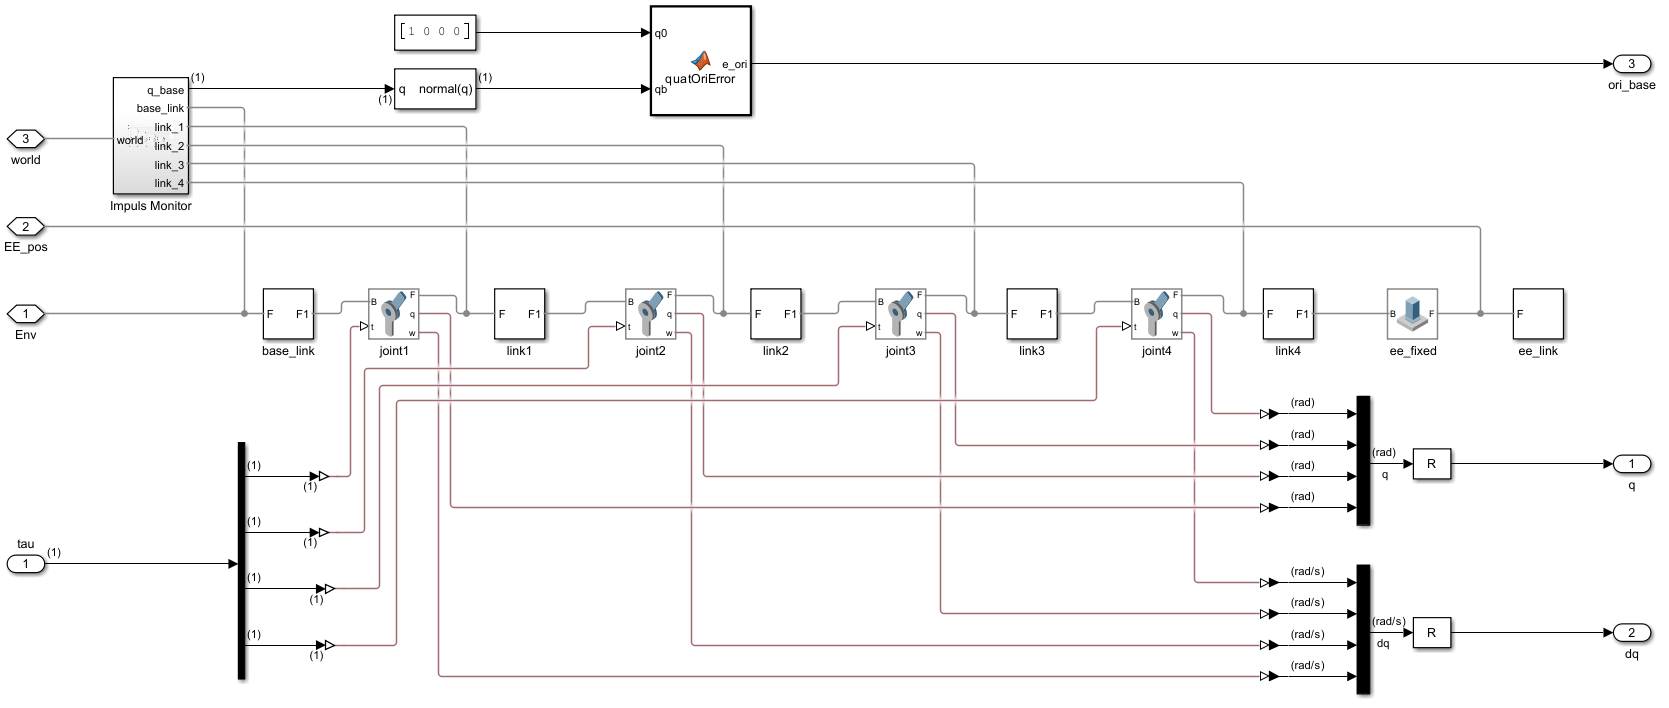
\includegraphics[width=0.98\linewidth]{Figures/spacerobot_slx_robot.png}
%DIFDELCMD < 	%%%
\DIFdelendFL \DIFaddbeginFL 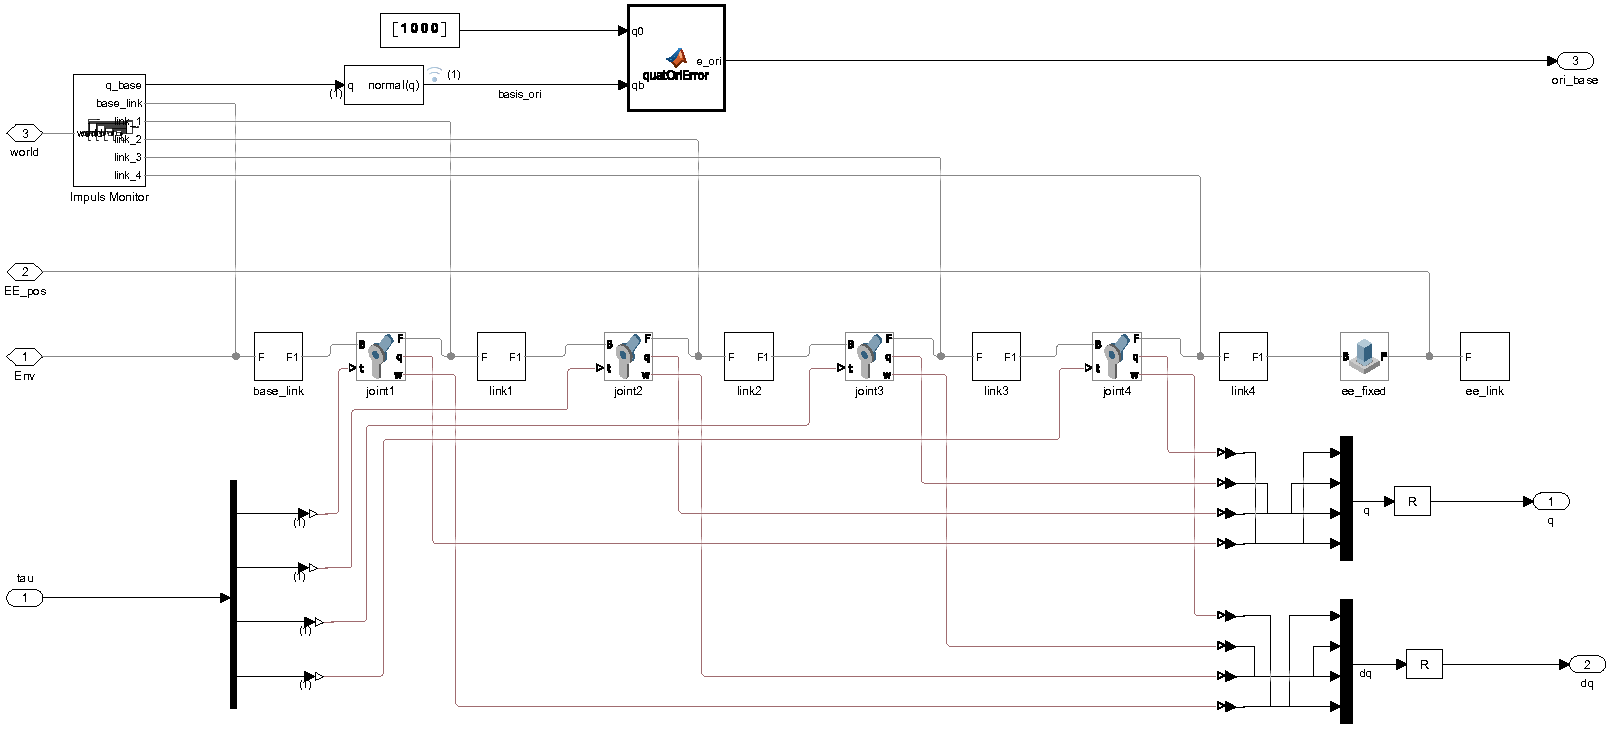
\includegraphics[width=0.98\linewidth]{Figures/spacerobot_slx_robot.pdf}
	\DIFaddendFL \caption{Overview of the Robot Subsystem in the Simulink Model \texttt{SpaceRobot.slx} \\
  This figure depicts the Simulink/Simscape Multibody model of the free-floating space robot, consisting of a floating base 
  and a serial 4-DOF manipulator. Joint torque commands are applied to the revolute joints, while joint positions and velocities 
  are measured and fed back as state variables. The base orientation is represented as a normalized quaternion and compared to a reference to compute the base attitude error.}
	\label{fig:spacerobot_slx_robot}
\end{figure*}

The Simulink model is composed of \DIFaddbegin \DIFadd{several }\DIFaddend subsystems, as illustrated in~\autoref{fig:spacerobot_slx}. The \emph{Robot Plant} subsystem computes
the \DIFdelbegin \DIFdel{full 6-DOF }\DIFdelend multibody dynamics of the free-floating robot at each time step (see~\autoref{fig:spacerobot_slx_robot}) \DIFdelbegin \DIFdel{, taking joint torque inputs 
and outputting the resulting robot states  }\DIFdelend by numerically integrating the equations of motion \DIFaddbegin \DIFadd{for the applied joint torques}\DIFaddend ~\cite{b6}. The \emph{Controller} subsystem executes the learned RL policy\DIFdelbegin \DIFdel{, 
applying joint torque commands that }\DIFdelend \DIFaddbegin \DIFadd{;
the commanded joint torques }\DIFaddend pass through saturation and safety verification blocks before reaching the plant. \DIFdelbegin \DIFdel{If }\DIFdelend \DIFaddbegin \DIFadd{When }\DIFaddend the collision monitor \DIFdelbegin \DIFdel{signals }\DIFdelend \DIFaddbegin \DIFadd{reports }\DIFaddend an imminent
collision, \DIFdelbegin \DIFdel{this block }\DIFdelend \DIFaddbegin \DIFadd{the controller }\DIFaddend issues an emergency stop and \DIFdelbegin \DIFdel{gradually overrides all }\DIFdelend \DIFaddbegin \DIFadd{overrides the }\DIFaddend torques to zero~\cite{b22,b23}. The \emph{Reference Trajectory Generator} provides the
desired end-effector trajectory and base attitude (see~\autoref{fig:spacerobot_slx_reference}), outputting the current target position and velocity at each time step.
\DIFdelbegin \DIFdel{Various }\DIFdelend \DIFaddbegin \DIFadd{A set of }\DIFaddend \emph{sensors} \DIFdelbegin \DIFdel{measure the robot 's }\DIFdelend \DIFaddbegin \DIFadd{measures the robot }\DIFaddend state (joint angles, \DIFaddbegin \DIFadd{joint }\DIFaddend velocities, base orientation, \DIFaddbegin \DIFadd{and }\DIFaddend base angular velocity) \DIFdelbegin \DIFdel{, combining them into an }\DIFdelend \DIFaddbegin \DIFadd{and assembles the }\DIFaddend observation signal for
the RL agent (detailed in \cref{RL}). Finally, \emph{safety monitors} enforce \DIFdelbegin \DIFdel{constraints. For instance, a Collision Monitor checks distances between robot components }\DIFdelend \DIFaddbegin \DIFadd{the operational constraints: a collision monitor compares the distance between selected robot components against a threshold $d_{\mathrm{safe}}$ }\DIFaddend and triggers a safety halt if \DIFdelbegin \DIFdel{any }\DIFdelend \DIFaddbegin \DIFadd{the }\DIFaddend distance falls below \DIFdelbegin \DIFdel{a threshold$d_{safe}$}\DIFdelend \DIFaddbegin \DIFadd{this threshold}\DIFaddend , while a joint-limit monitor triggers an emergency stop if any joint exceeds its \DIFdelbegin \DIFdel{allowed }\DIFdelend \DIFaddbegin \DIFadd{admissible }\DIFaddend range~\cite{b31,b22,b23}.

\begin{figure*}[!t]
	\centering
	\DIFdelbeginFL %DIFDELCMD < 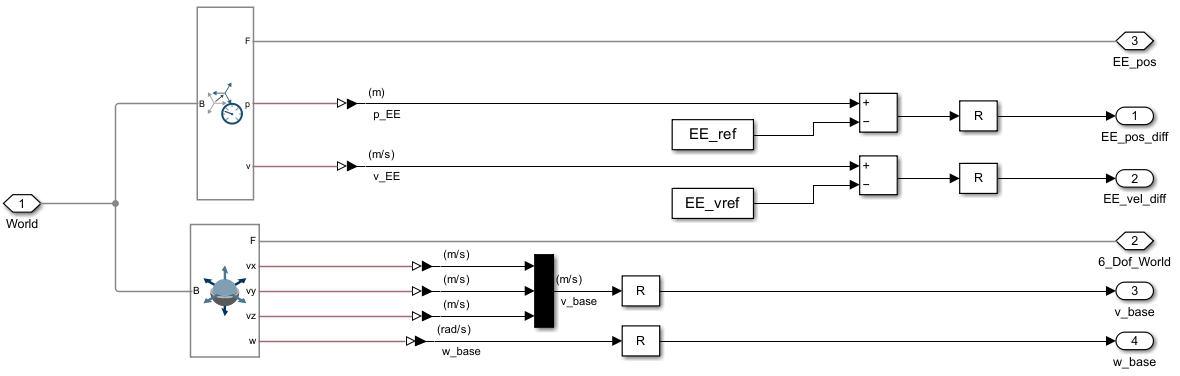
\includegraphics[width=0.97\linewidth]{Figures/spacerobot_slx_reference.png}
%DIFDELCMD < 	%%%
\DIFdelendFL \DIFaddbeginFL 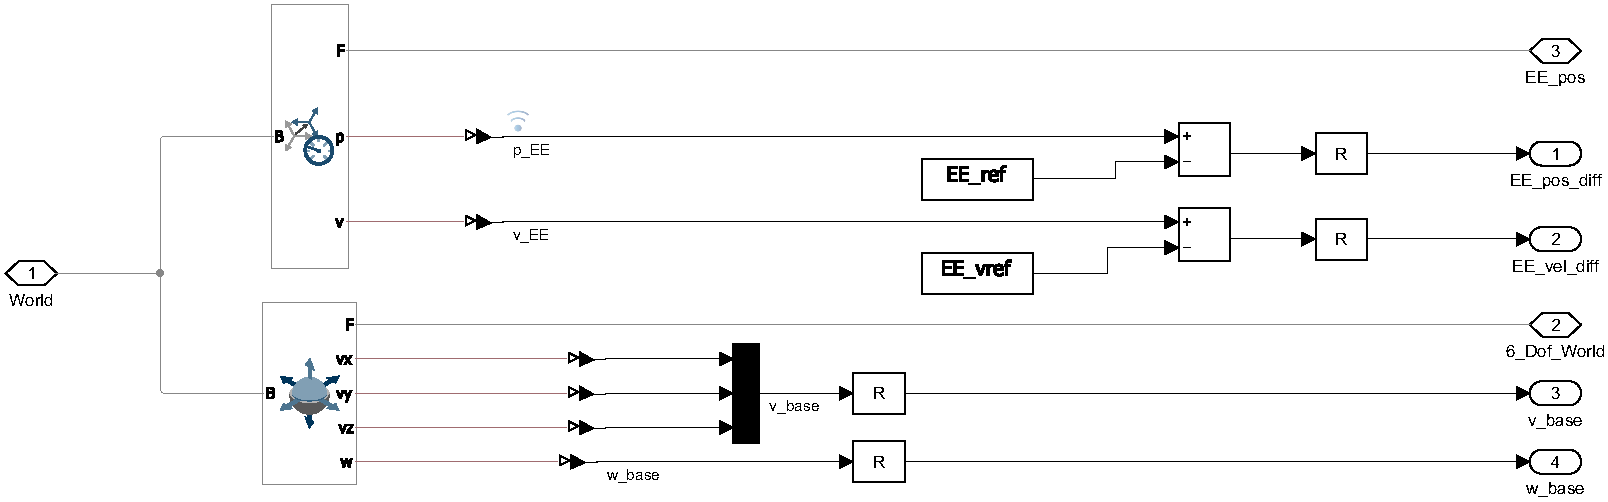
\includegraphics[width=0.97\linewidth]{Figures/spacerobot_slx_reference.pdf}
	\DIFaddendFL \caption{Overview of the Reference Subsystem in the Simulink Model \texttt{SpaceRobot.slx}\\
  This figure shows the computation of end-effector position and velocity tracking errors with respect to the reference trajectory. 
  The measured end-effector states are compared to the reference signals to generate position and velocity error vectors used for observation 
  and reward calculation. In addition, the base linear and angular velocities are extracted to capture base motion induced by manipulator actuation.}            
	\label{fig:spacerobot_slx_reference}
\end{figure*}

To \DIFdelbegin \DIFdel{accurately simulate }\DIFdelend \DIFaddbegin \DIFadd{couple }\DIFaddend the continuous dynamics \DIFdelbegin \DIFdel{while interfacing }\DIFdelend with the discrete-time RL agent, a
consistent integration scheme is used. The Simscape solver is configured \DIFdelbegin \DIFdel{to operate with a fixed-time
step }\DIFdelend \DIFaddbegin \DIFadd{with a fixed-step size
}\DIFaddend equal to the agent\DIFdelbegin \DIFdel{’}\DIFdelend \DIFaddbegin \DIFadd{'}\DIFaddend s decision interval ($\Delta t$) \DIFdelbegin \DIFdel{, }\DIFdelend instead of the default variable-step \DIFdelbegin \DIFdel{, to ensure
}\DIFdelend \DIFaddbegin \DIFadd{solver, ensuring
}\DIFaddend synchronization between the physics simulation and the RL decision\DIFdelbegin \DIFdel{-making}\DIFdelend  cycle. Rate
transition blocks handle \DIFdelbegin \DIFdel{any rate differences , avoiding aliasing and ensuring that state observations
and action commands align appropriately }\DIFdelend \DIFaddbegin \DIFadd{the remaining rate differences and prevent aliasing }\DIFaddend between the continuous plant and the discrete agent loop \cite{b29,b30}.
\DIFdelbegin \DIFdel{Additionally, Simulink ’s }\DIFdelend \DIFaddbegin \DIFadd{Simulink }\DIFaddend unit consistency checks are enabled to \DIFdelbegin \DIFdel{catch any modeling errors (e.g.
mismatched units ) }\DIFdelend \DIFaddbegin \DIFadd{detect modeling errors such as
mismatched units }\DIFaddend early in development.

\subsection{Reference Trajectory and Desired Task} The \DIFdelbegin \DIFdel{target task for the robot }\DIFdelend \DIFaddbegin \DIFadd{task }\DIFaddend is to follow a periodic end-effector
trajectory while minimizing \DIFdelbegin \DIFdel{the }\DIFdelend base disturbance. \DIFdelbegin \DIFdel{As previously mentioned, the }\DIFdelend \DIFaddbegin \DIFadd{The }\DIFaddend reference trajectory is \DIFdelbegin \DIFdel{chosen as }\DIFdelend a circular
path (see~\autoref{fig:ref_kreis_gesamt}). Prior to training\DIFdelbegin \DIFdel{the RL agents}\DIFdelend , the trajectory \DIFdelbegin \DIFdel{is }\DIFdelend \DIFaddbegin \DIFadd{was }\DIFaddend validated through inverse kinematics to \DIFdelbegin \DIFdel{ensure it is
geometrically feasible }\DIFdelend \DIFaddbegin \DIFadd{confirm geometric feasibility }\DIFaddend for the manipulator (\DIFdelbegin \DIFdel{within }\DIFdelend \DIFaddbegin \DIFadd{compliance with }\DIFaddend joint limits and \DIFdelbegin \DIFdel{avoiding }\DIFdelend \DIFaddbegin \DIFadd{absence of }\DIFaddend singularities). The \DIFdelbegin \DIFdel{inverse
kinematics solution produced }\DIFdelend \DIFaddbegin \DIFadd{inverse-kinematics solution yielded }\DIFaddend a consistent set of joint \DIFdelbegin \DIFdel{movements that achieve }\DIFdelend \DIFaddbegin \DIFadd{trajectories that realize }\DIFaddend the desired end-effector motion, confirming that the \DIFdelbegin \DIFdel{circle can be tracked by the arm without requiring unrealistic motions from a kinematic viewpoint}\DIFdelend \DIFaddbegin \DIFadd{circular path is kinematically feasible}\DIFaddend .
This precaution \DIFdelbegin \DIFdel{guarantees }\DIFdelend \DIFaddbegin \DIFadd{ensures }\DIFaddend that the task is achievable \DIFdelbegin \DIFdel{, at least by some }\DIFdelend \DIFaddbegin \DIFadd{by at least one }\DIFaddend controller, so \DIFdelbegin \DIFdel{if }\DIFdelend \DIFaddbegin \DIFadd{that any failure of }\DIFaddend the RL agent \DIFdelbegin \DIFdel{fails to learn it, it is due to learning limitations rather than an unattainable desired Cartesian poses of the end-effector}\DIFdelend \DIFaddbegin \DIFadd{can be attributed to learning, not to a kinematically infeasible reference}\DIFaddend . During simulation, the reference subsystem outputs the desired end-effector position and velocity
as time series \DIFdelbegin \DIFdel{$EE_{ref}(t)$ and $EE_{vref}(t)$ in the workspace }\DIFdelend \DIFaddbegin \DIFadd{$EE_{\mathrm{ref}}(t)$ and $EE_{v,\mathrm{ref}}(t)$ }\DIFaddend at each time step. \DIFdelbegin \DIFdel{From
these terms, the instantaneous tracking error signals are computed for the }\DIFdelend \DIFaddbegin \DIFadd{The instantaneous }\DIFaddend position and velocity \DIFdelbegin \DIFdel{of the end-effector. These error signals  are key components of the observation and are also
used in }\DIFdelend \DIFaddbegin \DIFadd{tracking errors are derived from these signals. They enter both the observation vector and }\DIFaddend the reward computation that penalizes large errors.
%DIF < , as described later. %The trajectory parameters (e.g., circle radius, speed, etc.) can be adjusted to adjust the task’s difficulty. For the experiments reported here, we choose moderate values that challenge the controller but do not push the arm to its dynamic limits.

%The simulation environment provides a flexible and challenging platform for learning, with a free-floating base, a non-trivial trajectory control task, and integrated mechanisms to measure performance and enforce safety. Next, we describe how the reinforcement learning problem is formulated in this environment.

\section{Reinforcement Learning Framework}\label{RL}
\DIFdelbegin \DIFdel{State (Observation) Space: The }\DIFdelend \DIFaddbegin \textbf{\DIFadd{State (Observation) Space.}} \DIFadd{At each time step the }\DIFaddend RL agent receives an observation \DIFdelbegin \DIFdel{capturing the system’s key state information relevant to control at each time step }\DIFdelend \DIFaddbegin \DIFadd{that summarizes the state variables relevant for control }\DIFaddend \cite{b7}. The state vector \DIFdelbegin \DIFdel{is composed }\DIFdelend \DIFaddbegin \DIFadd{consists }\DIFaddend of the following \DIFdelbegin \DIFdel{elements}\DIFdelend \DIFaddbegin \DIFadd{components}\DIFaddend :
\begin{itemize}
  \item \DIFdelbegin \DIFdel{End-Effector Tracking Error: The }\DIFdelend \DIFaddbegin \textit{\DIFadd{End-effector tracking error.}} \DIFadd{The Cartesian }\DIFaddend position error $e_p \in \mathbb{R}^3$ between the \DIFaddbegin \DIFadd{current and reference }\DIFaddend end-effector \DIFdelbegin \DIFdel{’s current position and the reference target position (in Cartesian coordinates). If }\DIFdelend \DIFaddbegin \DIFadd{positions, together with the velocity error $e_v \in \mathbb{R}^3$. When }\DIFaddend the
end-effector is \DIFdelbegin \DIFdel{exactly on the desired trajectorypoint, $e_{p} = 0$. Additionally, the error
in end-effector velocity $e_v \in \mathbb{R}^3$ (difference between current and target end-effector velocities) is included. Together, ($e_{p}$}\DIFdelend \DIFaddbegin \DIFadd{on the reference trajectory}\DIFaddend , \DIFdelbegin \DIFdel{$e_{v}$) provides the agent a
direct indication of tracking performance. Specifically, it tells the agent how far off the trajectory the end-effector is and whether it is lagging or overshooting in velocity }\DIFdelend \DIFaddbegin \DIFadd{$e_p = 0$. The pair $(e_p, e_v)$
indicates both the spatial deviation from the reference and the velocity mismatch}\DIFaddend .
  \item \DIFdelbegin \DIFdel{Arm Joint States: The positions and velocities of each of the 4 arm joints. We include the }\DIFdelend \DIFaddbegin \textit{\DIFadd{Arm joint states.}} \DIFadd{The }\DIFaddend joint angles $q \in \mathbb{R}^4$ and joint angular velocities \DIFdelbegin \DIFdel{$\dot q \in \mathbb{R}^4$ in the observation. These inform the agent about the manipulator’s }\DIFdelend \DIFaddbegin \DIFadd{$\dot{q} \in \mathbb{R}^4$. These describe the }\DIFaddend configuration and motion state \DIFdelbegin \DIFdel{(e.g., at rest or not). (Note: Joint angles can
be normalized or wrapped as needed, in our implementation they }\DIFdelend \DIFaddbegin \DIFadd{of the manipulator. Joint angles }\DIFaddend are provided in radians \DIFdelbegin \DIFdel{along
with known joint limits.
  )
  }\DIFdelend \DIFaddbegin \DIFadd{together with the corresponding mechanical limits.
  }\DIFaddend \item \DIFdelbegin \DIFdel{Base Motion: The free-floating }\DIFdelend \DIFaddbegin \textit{\DIFadd{Base motion.}} \DIFadd{The orientation, angular velocity, and linear velocity of the free-floating base. The }\DIFaddend base \DIFdelbegin \DIFdel{’s orientationand angular velocity. We parameterize the base’s orientation using quaternions. The }\DIFdelend \DIFaddbegin \DIFadd{attitude error is computed from the measured base quaternion $q_b$ and the reference }\DIFaddend quaternion \DIFdelbegin \DIFdel{\( q_{base} \in \mathbb{R}^4 \) describes the orientation of the base , capturing its attitude error from a reference orientation. }\DIFdelend \DIFaddbegin \DIFadd{$q_0$ as the relative quaternion $q_{\mathrm{err}} = q_0^{*} \otimes q_b$ (with sign convention enforcing a non-negative scalar part), and is then mapped to the axis--angle rotation vector $e_{\mathrm{ori}} = \theta\,\mathbf{u} \in \mathbb{R}^3$, where $\theta = 2\,\mathrm{atan2}(\|q_{\mathrm{err},v}\|,\,q_{\mathrm{err},w})$ and $\mathbf{u} = q_{\mathrm{err},v}/\|q_{\mathrm{err},v}\|$. This 3-dimensional minimal representation removes the redundancy of the unit-quaternion parameterization and is well-defined for $q_{\mathrm{err}} \neq \pm[1,0,0,0]^T$. }\DIFaddend Since the base is expected to maintain its initial attitude, \DIFdelbegin \DIFdel{the 
orientation error is ideally }\DIFdelend \DIFaddbegin \DIFadd{$e_{\mathrm{ori}}$ is }\DIFaddend kept near zero through the agent\DIFdelbegin \DIFdel{’}\DIFdelend \DIFaddbegin \DIFadd{'}\DIFaddend s actions. The base \DIFdelbegin \DIFdel{’s angular velocity $\omega_{base} \in \mathbb{R}^3$ is also included , as it
captures any ongoing rotation }\DIFdelend \DIFaddbegin \DIFadd{angular velocity $\omega_{\mathrm{base}} \in \mathbb{R}^3$ and the base linear velocity $v_{\mathrm{base}} \in \mathbb{R}^3$ are additionally included to capture residual rotation and momentum-coupled translation }\DIFaddend of the base.
%DIF < The base’s translational velocity could also be considered, however, in a free-floating scenario with no external forces and zero initial momentum, the center-of-mass linear velocity remains constant. In our case the base’s linear momentum is initially zero and remains near zero, so base translational motion is minimal by design. Thus, base linear velocity is not a major factor and can be omitted or included for completeness, our state focuses on rotational movement of the base.)
\end{itemize}
\DIFdelbegin %DIFDELCMD < \noindent
%DIFDELCMD < %%%
\DIFdel{Combining these components, the }\DIFdelend \DIFaddbegin 

\DIFadd{The }\DIFaddend overall observation vector has dimension \DIFdelbegin \DIFdel{$3 (e_{p}) + 3
(e_{v}) + 4 (q) + 4 (\dot q) + 3 (ori_{base}) + 3 (\omega_{base}) + 3 (v_{base}) = 23$ dimensions. This rich state description provides the agent with all
necessary information: how far the end-effector is from target, how the arm is configured/moving, and how the base is reacting}\DIFdelend \DIFaddbegin \DIFadd{$3(e_p) + 3(e_v) + 4(q) + 4(\dot{q}) + 3(\mathrm{ori}_{\mathrm{base}}) + 3(\omega_{\mathrm{base}}) + 3(v_{\mathrm{base}}) = 23$. This state representation contains the variables required by the agent to assess tracking deviation, arm configuration, and base motion}\DIFaddend .

\textbf{Action Space\DIFdelbegin \DIFdel{:}\DIFdelend \DIFaddbegin \DIFadd{.}\DIFaddend } The \DIFdelbegin \DIFdel{agent’s }\DIFdelend action is a vector of continuous joint torque commands\DIFdelbegin \DIFdel{for the
manipulator’s joints}\DIFdelend .
At each decision step, the agent outputs \DIFdelbegin \DIFdel{$a = [\tau_{1}~ \tau_{2}~
\tau_{3}~ \tau_{4}]^T$, corresponding to the torque to apply at each of the 4 revolute joints
}\DIFdelend \DIFaddbegin \DIFadd{$a = [\tau_{1},\, \tau_{2}, \tau_{3},\, \tau_{4}]^T$, with one component per revolute joint }\DIFaddend of the arm \cite{b2,b7}. The\DIFdelbegin \DIFdel{se}\DIFdelend  actions are real-valued and \DIFdelbegin \DIFdel{are constrained }\DIFdelend \DIFaddbegin \DIFadd{bounded }\DIFaddend by the actuator capabilities. \DIFdelbegin \DIFdel{We enforce
symmetric torque limits : each }\DIFdelend \DIFaddbegin \DIFadd{Symmetric torque limits }\DIFaddend $|\tau_{i}| \leq \tau_{\max}$ \DIFdelbegin \DIFdel{\text{(for i = 1..4)}. In the simulation, this
is implemented using }\DIFdelend \DIFaddbegin \DIFadd{for $i = 1,\ldots,4$ are enforced through }\DIFaddend saturation blocks that clip the commanded torque to the \DIFdelbegin \DIFdel{range }\DIFdelend \DIFaddbegin \DIFadd{interval }\DIFaddend $[-\tau_{\max}, +\tau_{\max}]$. The value of $\tau_{\max}$ is \DIFdelbegin \DIFdel{set based on the robot ’s design (for example, $\tau_{\max} = 25 Nm$ for all joints, though the exact value is not critical as long as it is sufficient }\DIFdelend \DIFaddbegin \DIFadd{selected according to the robot design ($\tau_{\max} = 25\,\mathrm{Nm}$ in this work), provided it is large enough }\DIFaddend to follow the \DIFdelbegin \DIFdel{trajectory). These saturation limits not only model physical actuator limits but also serve as a
safety measure to prevent excessive torques}\DIFdelend \DIFaddbegin \DIFadd{reference trajectory}\DIFaddend . \DIFaddbegin \DIFadd{The saturation enforces both the actuator limits and an upper bound on the applied torque for safety reasons. }\DIFaddend The action space is \DIFdelbegin \DIFdel{thus continuous }\DIFdelend \DIFaddbegin \DIFadd{therefore }\DIFaddend $\mathbb{R}^4$, \DIFdelbegin \DIFdel{making
this a continuous control problem that suits }\DIFdelend \DIFaddbegin \DIFadd{which is compatible with }\DIFaddend policy gradient and actor-critic \DIFdelbegin \DIFdel{RL }\DIFdelend methods.

The \DIFdelbegin \DIFdel{agent’s policy (the controller we are learning) }\DIFdelend \DIFaddbegin \DIFadd{policy }\DIFaddend is a mapping from the 23-dimensional state space to
the 4-dimensional action space\DIFdelbegin \DIFdel{: }\DIFdelend \DIFaddbegin \DIFadd{, }\DIFaddend $\pi: s \mapsto a$\DIFdelbegin \DIFdel{. Internally, this policy is represented }\DIFdelend \DIFaddbegin \DIFadd{, parameterized }\DIFaddend by a neural network whose parameters are adjusted during training to maximize \DIFaddbegin \DIFadd{the expected }\DIFaddend cumulative reward.
The \DIFdelbegin \DIFdel{control frequency (agent decision frequency) is chosen such that the agent outputs }\DIFdelend \DIFaddbegin \DIFadd{agent issues }\DIFaddend a new torque command at a fixed interval \DIFdelbegin \DIFdel{$\Delta t~$ (e.g., 0.1 s). This $\Delta t$ is the “agent sampling time” in Simulink and is
consistent with the simulation’s fixed step to maintain alignment}\DIFdelend \DIFaddbegin \DIFadd{$\Delta t = 0.1\,\mathrm{s}$, which coincides with the fixed simulation step size to ensure consistency between the discrete agent and the continuous plant}\DIFaddend .


\noindent
\textbf{Reward Function Design\DIFdelbegin \DIFdel{:}\DIFdelend \DIFaddbegin \DIFadd{.}\DIFaddend } \DIFdelbegin \DIFdel{A crucial aspect of the reinforcement learning formulation is the reward signal , which }\DIFdelend \DIFaddbegin \DIFadd{The reward signal }\DIFaddend guides the agent toward accurate trajectory tracking
while minimizing base disturbance and enforcing smooth, \DIFdelbegin \DIFdel{safe }\DIFdelend \DIFaddbegin \DIFadd{bounded }\DIFaddend control actions.
At each discrete time step $t$, the reward $r_t$ is computed as the sum of a progress term and a proximity bonus, minus a weighted cost function:
\begin{equation}
r_t = \frac{1}{C}\left( r_{\text{prog}} + r_{\text{bonus}} - c_t \right),
\label{eq:reward}
\end{equation}
where $C$ is a normalization constant.

To encourage monotonic convergence toward the reference trajectory, a progress reward is defined based on the reduction of the end-effector position error:
\begin{equation}
r_{\text{prog}} = 
\begin{cases}
k_p \left( d_{t-1} - d_t \right), & d_{t-1} > d_t,\\
0, & \text{otherwise},
\end{cases}
\end{equation}
where $d_t = \|e_p(t)\|$ is the Euclidean end-effector position error and $k_p$ is a scaling factor. The previous distance $d_{t-1}$ is stored persistently across time steps.

A small shaping bonus is added when the end-effector is close to the reference point:
\begin{equation}
r_{\text{bonus}} = k_b \exp\!\left(-\left(\frac{d_t}{\sigma}\right)^2\right),
\end{equation}
which improves local convergence behavior near the desired trajectory.

The instantaneous cost $c_t$ penalizes tracking errors, base motion, and control effort:
\begin{align}
c_t =&\;
W_p \|e_p\|^2
+ W_v \|e_v\|^2
+ W_{\text{ori}} \|e_{\text{ori}}\|^2
+ W_{\omega_b} \|\omega_{\text{base}}\|^2 \nonumber \\
&+ W_{v_b} \|v_{\text{base}}\|^2
+ W_u \|\tau\|^2
+ W_d \|\tau - \tau_{t-1}\|^2 ,
\end{align}
where $e_p$ and $e_v$ denote the end-effector position and velocity errors, $e_{\text{ori}}$ the base orientation error, $v_{\text{base}}$ and $\omega_{\text{base}}$ the linear 
and angular base velocities, and $\tau$ the joint torque vector. The final term penalizes changes in control input to promote smooth actuation.

The weights used in all experiments are summarized in~\autoref{tab:reward_weights}.
\DIFdelbegin \DIFdel{High weights are assigned to }\DIFdelend \DIFaddbegin \DIFadd{The physical intuition behind the weight choices is as follows.
The }\DIFaddend end-effector \DIFdelbegin \DIFdel{tracking and base orientation preservation, while control effort and }\DIFdelend \DIFaddbegin \DIFadd{position error weight $W_p = 150$ is large because trajectory tracking is the primary task objective. A high weight makes the position error the dominant term of the cost at typical error magnitudes.
The velocity error weight $W_v = 25$ is lower than $W_p$ to avoid over-penalizing transient dynamics during fast arm motion, while still discouraging persistent velocity offsets.
The base orientation weight $W_{\text{ori}} = 200$ is the largest in the cost function, reflecting that base attitude disturbance is safety-critical in on-orbit operations. Any uncontrolled rotation of the spacecraft base can jeopardize mission success independently of tracking performance.
The base angular velocity weight $W_{\omega_b} = 8$ provides a damping-like penalty on ongoing base rotation, while the linear velocity weight $W_{v_b} = 2$ is kept small because, in a free-floating system initialized with zero total linear momentum, base translation is momentum-coupled to the manipulator motion and is expected to remain limited for the considered task configuration. Recall that manipulator motion can induce base translation because the total system center of mass is conserved. The torque magnitude weight $W_u = 0.02$ and }\DIFaddend torque-rate \DIFdelbegin \DIFdel{penalties are kept comparatively small to allow sufficient exploration. }\DIFdelend \DIFaddbegin \DIFadd{weight $W_d = 0.06$ are intentionally small to leave the agent sufficient freedom to explore diverse control actions. The torque-rate penalty is slightly larger to specifically discourage high-frequency chattering in the control signal.
The progress scaling factor $k_p = 10$ is chosen so that the progress reward is of comparable magnitude to the cost terms at typical error levels, preventing it from being dominated.
The proximity bonus parameters $k_b = 0.05$ and $\sigma = 0.02$ are small by design. They provide a weak local guidance signal near the trajectory without creating a strong local attractor that could trap the policy.
Finally, the normalization constant $C = 500$ scales the total reward to a range of approximately $[-1,\, 0]$ under typical operating conditions, which stabilizes value function learning across all tested algorithms.
}\DIFaddend 

At each step, all inputs to the reward function are checked for numerical validity. If any NaN or Inf values are detected, or if the end-effector error exceeds a predefined bound, the episode is immediately terminated and a terminal \DIFdelbegin \DIFdel{reward of $-1$ }\DIFdelend \DIFaddbegin \DIFadd{penalty of $r_{\text{fail}} = -1$ }\DIFaddend is assigned. This \DIFdelbegin \DIFdel{mechanism prevents the agent from exploiting invalid states and ensures numerical robustness during training. }\DIFdelend \DIFaddbegin \DIFadd{value is matched to the reward scale. With the normalization constant $C = 500$, typical step rewards lie approximately in $[-1,\,0]$, so $r_{\text{fail}} = -1$ corresponds to the lower end of the one-step reward range. The penalty is therefore large enough to discourage invalid states without dominating the cumulative return over an entire episode. A much smaller penalty (e.g., $-0.1$) would provide a weak failure signal, whereas a much larger penalty (e.g., $-100$) could overshadow the remaining reward terms and destabilize value-function learning. Anchoring the failure penalty to the step-reward scale yields a balanced failure signal for policy optimization.
}\DIFaddend All reward components were implemented in a MATLAB Function block within the Simulink environment.
\DIFdelbegin \DIFdel{The weights were tuned empirically to provide informative gradients while maintaining stable learning behavior.
}\DIFdelend 

\begin{table}[!b]
\centering
\caption{Reward function weights used in all experiments.}
\label{tab:reward_weights}
\begin{tabular}{lcc}
\toprule
\textbf{Term} & \textbf{Symbol} & \textbf{Value} \\
\midrule
End-effector position error      & $W_p$              & 150   \\
End-effector velocity error      & $W_v$              & 25    \\
Base orientation error           & $W_{\text{ori}}$   & 200   \\
Base angular velocity            & $W_{\omega_b}$     & 8     \\
Base linear velocity             & $W_{v_b}$          & 2     \\
Joint torque magnitude           & $W_u$              & 0.02  \\
Torque rate (smoothness)         & $W_d$              & 0.06  \\
Progress scaling factor          & $k_p$              & 10    \\
Proximity bonus scaling          & $k_b$              & 0.05  \\
Proximity width                  & $\sigma$           & 0.02  \\
Reward normalization constant    & $C$                & 500   \\
\bottomrule
\end{tabular}
\end{table}

\textbf{Training Procedure\DIFdelbegin \DIFdel{:}\DIFdelend \DIFaddbegin \DIFadd{.}\DIFaddend } \DIFdelbegin \DIFdel{We adopt an episodic training approach}\DIFdelend \DIFaddbegin \DIFadd{An episodic training scheme is used}\DIFaddend . Each episode corresponds to a
simulation of fixed duration\DIFdelbegin \DIFdel{. A finite horizon of H }\DIFdelend \DIFaddbegin \DIFadd{, either a horizon of $H$ }\DIFaddend seconds or a fixed number of time steps \DIFdelbegin \DIFdel{N. In our case, }\DIFdelend \DIFaddbegin \DIFadd{$N$, chosen such that
one episode covers }\DIFaddend one \DIFdelbegin \DIFdel{episode lasts long enough for the end-effector to attempt following the circular trajectory (e.g., one
}\DIFdelend or two \DIFdelbegin \DIFdel{loops of the circle)}\DIFdelend \DIFaddbegin \DIFadd{laps of the circular reference}\DIFaddend . At the start of each episode, the system is reset to an \DIFaddbegin \DIFadd{admissible }\DIFaddend initial condition by a
custom reset function. The initial joint angles are set to a feasible configuration \DIFdelbegin \DIFdel{(e.g., the arm in a
certain pose near the }\DIFdelend \DIFaddbegin \DIFadd{close to the }\DIFaddend start of the trajectory \DIFdelbegin \DIFdel{) }\DIFdelend and the base is \DIFdelbegin \DIFdel{at }\DIFdelend \DIFaddbegin \DIFadd{set to }\DIFaddend a defined attitude (\DIFdelbegin \DIFdel{often }\DIFdelend the home orientation\DIFdelbegin \DIFdel{and }\DIFdelend \DIFaddbegin \DIFadd{, }\DIFaddend at rest). All state variables, \DIFdelbegin \DIFdel{observer
integrators}\DIFdelend \DIFaddbegin \DIFadd{integrator states}\DIFaddend , and logging signals are reset\DIFdelbegin \DIFdel{. We ensure }\DIFdelend \DIFaddbegin \DIFadd{, and }\DIFaddend the initial state is \DIFdelbegin \DIFdel{within safe bounds }\DIFdelend \DIFaddbegin \DIFadd{verified to lie within the safe set }\DIFaddend (no collisions or limit violations at \DIFdelbegin \DIFdel{t=0}\DIFdelend \DIFaddbegin \DIFadd{$t = 0$}\DIFaddend ). The reset function \DIFdelbegin \DIFdel{can randomize }\DIFdelend \DIFaddbegin \DIFadd{supports randomization of }\DIFaddend the starting joint angles \DIFdelbegin \DIFdel{within a
range or the phase of the trajectory }\DIFdelend \DIFaddbegin \DIFadd{and the trajectory phase }\DIFaddend to improve generalization\DIFdelbegin \DIFdel{, though within this study , we kept a consistent start pose for simplicity (}\DIFdelend \DIFaddbegin \DIFadd{. In this study a fixed start pose is used, }\DIFaddend with the end-effector \DIFdelbegin \DIFdel{at a specific }\DIFdelend \DIFaddbegin \DIFadd{placed at a defined }\DIFaddend point on the circle \DIFdelbegin \DIFdel{) }\DIFdelend \cite{b7}.

\DIFdelbegin \DIFdel{Once an episodebegins}\DIFdelend \DIFaddbegin \DIFadd{Within an episode}\DIFaddend , the agent receives \DIFdelbegin \DIFdel{observations }\DIFdelend \DIFaddbegin \DIFadd{an observation }\DIFaddend at each step and outputs \DIFdelbegin \DIFdel{torque actions}\DIFdelend \DIFaddbegin \DIFadd{a torque action}\DIFaddend . The
simulation runs until \DIFdelbegin \DIFdel{either }\DIFdelend the time horizon \DIFdelbegin \DIFdel{is reached (the episode length H) }\DIFdelend \DIFaddbegin \DIFadd{$H$ is reached }\DIFaddend or a terminal condition occurs (task \DIFdelbegin \DIFdel{completed }\DIFdelend \DIFaddbegin \DIFadd{completion }\DIFaddend or safety violation). \DIFdelbegin \DIFdel{As described, reaching the end of the trajectory successfully
or experiencing a failure condition will terminate the episode prematurely. In practice, an episode might end early if}\DIFdelend \DIFaddbegin \DIFadd{An early termination is triggered}\DIFaddend , for example, \DIFaddbegin \DIFadd{when }\DIFaddend the agent causes a collision \DIFdelbegin \DIFdel{at 70\% of the trajectory, it will receive the penalty }\DIFdelend \DIFaddbegin \DIFadd{before completing the trajectory. The corresponding terminal penalty is applied }\DIFaddend and the episode \DIFdelbegin \DIFdel{stops there}\DIFdelend \DIFaddbegin \DIFadd{ends at that instant}\DIFaddend .

\DIFdelbegin \DIFdel{We use a }\DIFdelend \DIFaddbegin \DIFadd{The training loop is the }\DIFaddend standard policy gradient \DIFdelbegin \DIFdel{training loop (as }\DIFdelend \DIFaddbegin \DIFadd{procedure }\DIFaddend provided by MATLAB\DIFdelbegin \DIFdel{’s RL toolbox): after }\DIFdelend \DIFaddbegin \DIFadd{'s Reinforcement Learning Toolbox. After }\DIFaddend each episode (or after a \DIFdelbegin \DIFdel{set }\DIFdelend \DIFaddbegin \DIFadd{fixed }\DIFaddend number of steps), the collected state, action, \DIFaddbegin \DIFadd{and }\DIFaddend reward trajectories are used to
update the \DIFdelbegin \DIFdel{agent’s }\DIFdelend policy (and \DIFaddbegin \DIFadd{the }\DIFaddend value function, \DIFdelbegin \DIFdel{if applicable) via }\DIFdelend \DIFaddbegin \DIFadd{where applicable) according to }\DIFaddend the chosen RL algorithm \cite{b4}. The \DIFdelbegin \DIFdel{particularities of each algorithm (}\DIFdelend \DIFaddbegin \DIFadd{algorithm-specific update rules of }\DIFaddend PPO, DDPG, \DIFdelbegin \DIFdel{etc.) }\DIFdelend \DIFaddbegin \DIFadd{and the remaining methods }\DIFaddend are handled by their respective \DIFdelbegin \DIFdel{implementation, we supply }\DIFdelend \DIFaddbegin \DIFadd{toolbox implementations. This work supplies }\DIFaddend the experience and \DIFdelbegin \DIFdel{let the algorithm update the neural network }\DIFdelend \DIFaddbegin \DIFadd{the reward signal }\DIFaddend \cite{b7}.
All agents \DIFdelbegin \DIFdel{were }\DIFdelend \DIFaddbegin \DIFadd{are }\DIFaddend trained for the same number of episodes\DIFdelbegin \DIFdel{to allow fair comparison. We chose
$N_{train} = 1000$ episodes for each agent, which was }\DIFdelend \DIFaddbegin \DIFadd{, $N_{\mathrm{train}} = 1000$, which is }\DIFaddend sufficient for most algorithms to
converge or reach a performance plateau. During training \DIFdelbegin \DIFdel{, we monitored metrics such as the cumulative reward per episode , }\DIFdelend the \DIFaddbegin \DIFadd{cumulative episode reward, the mean }\DIFaddend end-effector tracking error, and the \DIFdelbegin \DIFdel{base motion, averaged over
each }\DIFdelend \DIFaddbegin \DIFadd{mean base motion are recorded per }\DIFaddend episode. A successful training run is characterized by \DIFdelbegin \DIFdel{the episode reward increasing (toward 0,
since }\DIFdelend \DIFaddbegin \DIFadd{an episode return that increases toward zero (}\DIFaddend negative costs are used) and \DIFaddbegin \DIFadd{by a decrease of }\DIFaddend the tracking error and base \DIFdelbegin \DIFdel{movement decreasing }\DIFdelend \DIFaddbegin \DIFadd{motion }\DIFaddend over time. \DIFdelbegin \DIFdel{We
also tracked the }\DIFdelend \DIFaddbegin \DIFadd{The }\DIFaddend number of episodes \DIFdelbegin \DIFdel{that ended prematurely due to safety triggers, aiming for this to go }\DIFdelend \DIFaddbegin \DIFadd{terminated prematurely by the safety monitors is also tracked and expected to decrease }\DIFaddend to zero as training progresses.

\DIFdelbegin \DIFdel{For each algorithm, we performed multiple training runs and selected the best-performing policy (based on highest average reward achieved) for final evaluation. We found relatively consistent results }\DIFdelend \DIFaddbegin \DIFadd{To ensure reproducibility, all training runs were initialized using MATLAB's Mersenne Twister random number generator with a fixed seed of zero (}\texttt{\DIFadd{rng(0,`twister')}}\DIFadd{), applied prior to each training session. For each of the six algorithms, }\textbf{\DIFadd{three independent training runs}} \DIFadd{were performed under identical conditions, namely the same environment, reward function, episode length, and initial state. This resulted in 18 training runs in total. The policy selection procedure was as follows. After all three runs per algorithm completed, the policy checkpoint achieving the highest mean episodic reward over the final 50 training episodes was identified. This checkpoint was then used exclusively for all subsequent evaluation experiments. The results were relatively consistent }\DIFaddend across runs for the more stable algorithms (PPO, TRPO), whereas some runs of \DIFaddbegin \DIFadd{the }\DIFaddend less stable methods (e.g.\DIFdelbegin \DIFdel{DDPG) would diverge, underscoring }\DIFdelend \DIFaddbegin \DIFadd{\ DDPG) diverged, which underlines }\DIFaddend the importance of \DIFdelbegin \DIFdel{stability}\DIFdelend \DIFaddbegin \DIFadd{algorithmic stability in this setting}\DIFaddend .

\textbf{Evaluation and Metrics\DIFdelbegin \DIFdel{:}\DIFdelend \DIFaddbegin \DIFadd{.}\DIFaddend } After training, \DIFdelbegin \DIFdel{we evaluated each agent’s performance }\DIFdelend \DIFaddbegin \DIFadd{each agent's performance was evaluated }\DIFaddend on $N_{eval}
= 30$ independent episodes \DIFdelbegin \DIFdel{(with various initial conditions) to gather statistics}\DIFdelend \DIFaddbegin \DIFadd{from a fixed initial configuration}\DIFaddend . Over these
evaluation runs, \DIFdelbegin \DIFdel{we compute }\DIFdelend a set of Key Performance Indicators (KPIs) \DIFdelbegin \DIFdel{to quantitatively }\DIFdelend \DIFaddbegin \DIFadd{was computed to }\DIFaddend compare the
agents \DIFdelbegin \DIFdel{. These KPIs include: 
}\DIFdelend \DIFaddbegin \DIFadd{quantitatively. For episodes that terminate early due to a safety violation, each KPI is computed over the executed portion of the episode up to the termination step.
}\DIFaddend 

\DIFaddbegin \DIFadd{The nine KPIs are organized into three groups to aid interpretation. The }\emph{\DIFadd{tracking accuracy}} \DIFadd{group ($K_2$ and $K_3$) measures how closely the end-effector follows the reference path. The }\emph{\DIFadd{base stability and safety}} \DIFadd{group covers spacecraft attitude drift ($K_4$) and constraint violations ($K_5$ and $K_6$). The }\emph{\DIFadd{efficiency}} \DIFadd{group covers control smoothness ($K_7$), residual base rotation ($K_8$), and energy consumption ($K_9$). $K_1$ serves as an overall scalar summary of the agent's performance across all objectives, since it is the cumulative reward that jointly penalizes all undesired behaviors.
}

\DIFaddend \begin{itemize}
  \item \DIFdelbegin \DIFdel{K1: Average Episodic Return, the mean }\DIFdelend \DIFaddbegin \textbf{\DIFadd{K1}} \DIFadd{(}\emph{\DIFadd{Average Episodic Return}}\DIFadd{). Mean }\DIFaddend cumulative reward per episode\DIFdelbegin \DIFdel{(higher is better , this reflects overall success in the task ).
  }%DIFDELCMD < \\
%DIFDELCMD <   %%%
\DIFdel{$R_i=\sum_{k=1}^{T_i} r_i[k], \\ \qquad K1=\frac{1}{N_{eval}}\sum_{i=1}^{N_{eval}} R_i.$
}\DIFdelend \DIFaddbegin \DIFadd{. Higher is better and reflects overall task success.
  }\begin{equation*}
  \DIFadd{R_i=\sum_{k=1}^{T_i} r_i[k], \qquad K1=\frac{1}{N_{\text{eval}}}\sum_{i=1}^{N_{\text{eval}}} R_i.
  }\end{equation*}
\DIFaddend 

  \item \DIFdelbegin \DIFdel{K2: Mean Squared End-Effector Position Error, averaged over the episode (lower is better, measures tracking accuracy).
  }%DIFDELCMD < \\
%DIFDELCMD <   %%%
\DIFdel{$K2=\frac{1}{N_{eval}}\sum_{i=1}^{N_{eval}}\frac{1}{T_i}\sum_{k=1}^{T_i}\|e_{p,i}[k]\|_2^2.$
}\DIFdelend \DIFaddbegin \textbf{\DIFadd{K2}} \DIFadd{(}\emph{\DIFadd{Mean Squared EE Position Error}}\DIFadd{). Average squared tracking error per episode. Lower is better.
  }\begin{equation*}
  \DIFadd{K2=\frac{1}{N_{\text{eval}}}\sum_{i=1}^{N_{\text{eval}}}\frac{1}{T_i}\sum_{k=1}^{T_i}\|e_{p,i}[k]\|_2^2.
  }\end{equation*}
\DIFaddend 

  \item \DIFdelbegin \DIFdel{K3: Maximum End-Effector Position Error, worst-case deviation during the episode (lower is better}\DIFdelend \DIFaddbegin \textbf{\DIFadd{K3}} \DIFadd{(}\emph{\DIFadd{Maximum EE Position Error}}\DIFaddend ). \DIFdelbegin %DIFDELCMD < \\
%DIFDELCMD <   %%%
\DIFdel{$K3=\max_{i}\max_{k}\|e_{p,i}[k]\|_2.$
}\DIFdelend \DIFaddbegin \DIFadd{Worst-case tracking deviation. Lower is better.
  }\begin{equation*}
  \DIFadd{K3=\max_{i}\max_{k}\|e_{p,i}[k]\|_2.
  }\end{equation*}
\DIFaddend 

  \item \DIFdelbegin \DIFdel{K4: Mean Base Orientation Error, e.g., average quaternion error magnitude indicating how far the base drifted in attitude (lower is better).
  }%DIFDELCMD < \\
%DIFDELCMD <   %%%
\DIFdel{$K4=\frac{1}{N_{eval}}\sum_{i=1}^{N_{eval}}\frac{1}{T_i}\sum_{k=1}^{T_i}\|e_{R,i}[k]\|_2.$
}\DIFdelend \DIFaddbegin \textbf{\DIFadd{K4}} \DIFadd{(}\emph{\DIFadd{Mean Base Orientation Error}}\DIFadd{). Average attitude drift of the spacecraft base, measured as the magnitude of the axis--angle rotation-vector error $e_{\mathrm{ori}}$ (in radians). Lower is better.
  }\begin{equation*}
  \DIFadd{K4=\frac{1}{N_{\text{eval}}}\sum_{i=1}^{N_{\text{eval}}}\frac{1}{T_i}\sum_{k=1}^{T_i}\|e_{\mathrm{ori},i}[k]\|_2.
  }\end{equation*}
\DIFaddend 

  \item \DIFdelbegin \DIFdel{K5: Collision Rate, the fraction of episodes in which }\DIFdelend \DIFaddbegin \textbf{\DIFadd{K5}} \DIFadd{(}\emph{\DIFadd{Collision Rate}}\DIFadd{). Fraction of episodes with }\DIFaddend at least one collision\DIFdelbegin \DIFdel{occurred (0 means no collisions, we expect this to be zero if the agent behaves safely). }%DIFDELCMD < \\
%DIFDELCMD <   %%%
\DIFdel{$C_i=\mathbb{I}(\exists k:\,c_i[k]>0.5), \\ \qquad K5=\frac{1}{N_{eval}}\sum_{i=1}^{N_{eval}} C_i.$
}\DIFdelend \DIFaddbegin \DIFadd{. Zero is ideal.
  }\begin{equation*}
  \DIFadd{C_i=\mathbb{I}(\exists k:\,c_i[k]>0.5), \qquad K5=\frac{1}{N_{\text{eval}}}\sum_{i=1}^{N_{\text{eval}}} C_i.
  }\end{equation*}
\DIFaddend 

  \item \DIFdelbegin \DIFdel{K6: Joint Limit Violation Rate (0 is ideal).
  }%DIFDELCMD < \\
%DIFDELCMD <   %%%
\DIFdel{$K6=\frac{1}{N_{eval}}\sum_{i=1}^{N_{eval}}\frac{1}{T_i n_J}\sum_{k=1}^{T_i}\sum_{j=1}^{n_J}
  \mathbb{I}\!\big(q_{i,j}[k]\notin[q_j^{\min},q_j^{\max}]\big).$
}\DIFdelend \DIFaddbegin \textbf{\DIFadd{K6}} \DIFadd{(}\emph{\DIFadd{Joint Limit Violation Rate}}\DIFadd{). Fraction of time steps across episodes where any joint exceeds its mechanical limit. Zero is ideal.
  }\begin{equation*}
  \DIFadd{K6=\frac{1}{N_{\text{eval}}}\sum_{i=1}^{N_{\text{eval}}}\frac{1}{T_i n_J}\sum_{k=1}^{T_i}\sum_{j=1}^{n_J}
  \mathbb{I}\!\big(q_{i,j}[k]\notin[q_j^{\min},q_j^{\max}]\big).
  }\end{equation*}
\DIFaddend 

  \item \DIFdelbegin \DIFdel{K7: Control Smoothness (Jerk), a measure of actuation smoothness, computed as the second }\DIFdelend \DIFaddbegin \textbf{\DIFadd{K7}} \DIFadd{(}\emph{\DIFadd{Control Smoothness (Jerk)}}\DIFadd{). Second }\DIFaddend difference of joint torques. Lower values indicate smoother\DIFdelbegin \DIFdel{control.
  }%DIFDELCMD < \\
%DIFDELCMD <   %%%
\DIFdel{$\Delta^2\tau_i[k]=\tau_i[k+2]-2\tau_i[k+1]+\tau_i[k], \\\qquad
  K7=\frac{1}{N_{eval}}\sum_{i=1}^{N_{eval}}\frac{1}{T_i-2}\sum_{k=1}^{T_i-2}\|\Delta^2\tau_i[k]\|_2.$
}\DIFdelend \DIFaddbegin \DIFadd{, less chattering actuation.
  }\begin{equation*}
  \DIFadd{\begin{aligned}
  \Delta^2\tau_i[k] &= \tau_i[k+2]-2\tau_i[k+1]+\tau_i[k],\\
  J_i &= \frac{1}{T_i-2}\sum_{k=1}^{T_i-2}\|\Delta^2\tau_i[k]\|_2,\\
  K7 &= \frac{1}{N_{\text{eval}}}\sum_{i=1}^{N_{\text{eval}}}J_i.
  \end{aligned}
  }\end{equation*}
\DIFaddend 

  \item \DIFdelbegin \DIFdel{K8: Mean Base Angular Velocity, a measure of residual base rotation (rad/s)}\DIFdelend \DIFaddbegin \textbf{\DIFadd{K8}} \DIFadd{(}\emph{\DIFadd{Mean Base Angular Velocity}}\DIFadd{). Residual spacecraft rotation rate }\DIFaddend during the task (\DIFdelbegin \DIFdel{lower }\DIFdelend \DIFaddbegin \DIFadd{rad/s). Lower }\DIFaddend is better, ideally zero\DIFdelbegin \DIFdel{).
  }%DIFDELCMD < \\
%DIFDELCMD <   %%%
\DIFdel{$K8=\frac{1}{N_{eval}}\sum_{i=1}^{N_{eval}}\frac{1}{T_i}\sum_{k=1}^{T_i}\|\omega_{b,i}[k]\|_2.$
}\DIFdelend \DIFaddbegin \DIFadd{.
  }\begin{equation*}
  \DIFadd{K8=\frac{1}{N_{\text{eval}}}\sum_{i=1}^{N_{\text{eval}}}\frac{1}{T_i}\sum_{k=1}^{T_i}\|\omega_{b,i}[k]\|_2.
  }\end{equation*}
\DIFaddend 

  \item \DIFdelbegin \DIFdel{K9: Energy Consumption, approximate average energy expended }\DIFdelend \DIFaddbegin \textbf{\DIFadd{K9}} \DIFadd{(}\emph{\DIFadd{Energy Consumption}}\DIFadd{). Average absolute mechanical power integrated over each episode. Lower is better when not at the expense of tracking quality.
  }\begin{equation*}
  \DIFadd{E_i=\int\sum_{j=1}^{n_J}\big|\tau_{i,j}(t)\,\dot q_{i,j}(t)\big|\,dt, \qquad
  K9=\frac{1}{N_{\text{eval}}}\sum_{i=1}^{N_{\text{eval}}} E_i.
  }\end{equation*}
\end{itemize}


\DIFadd{Two KPIs deserve explicit justification in the space mission context. }\textbf{\DIFadd{K7 (Control Smoothness)}} \DIFadd{captures high-frequency torque oscillations (chattering). In space, such oscillations can accelerate actuator wear, excite structural vibrations that degrade the pointing accuracy of sensitive instruments such as cameras or star trackers, and dissipate energy through rapid back-and-forth motion. Minimizing $K_7$ therefore supports hardware lifetime and payload pointing requirements. }\textbf{\DIFadd{K9 (Energy Consumption)}} \DIFadd{reflects the mechanical work performed }\DIFaddend by the joints\DIFdelbegin \DIFdel{(e.g., $\int(\tau \cdot \dot q) dt$ using an absolute-power proxy). Lower energy usage 
  is better if achieved without sacrificing performance.
}%DIFDELCMD < \\
%DIFDELCMD <   %%%
\DIFdel{$E_i=\int\sum_{j=1}^{n_J}\big|\tau_{i,j}(t)\dot q_{i,j}(t)\big|\,dt, \\\qquad
  K9=\frac{1}{N_{eval}}\sum_{i=1}^{N_{eval}} E_i.$
}%DIFDELCMD < \end{itemize}
%DIFDELCMD < %%%
\DIFdelend \DIFaddbegin \DIFadd{, approximated as $\int |\tau \cdot \dot{q}|\,dt$. Onboard power is limited by solar panel area and battery capacity. Energy spent on control actuation reduces the budget available for communication, thermal management, and payload operation. Reducing $K_9$ without sacrificing tracking accuracy therefore has operational value for mission planning.
}\DIFaddend 

\DIFdelbegin %DIFDELCMD < \noindent
%DIFDELCMD < %%%
\DIFdel{Additionally, we consider }\DIFdelend \DIFaddbegin \DIFadd{In addition to the KPIs above, three }\DIFaddend training-related metrics \DIFdelbegin \DIFdel{for comparison: T1: }\DIFdelend \DIFaddbegin \DIFadd{are reported. $T_1$ is the }\DIFaddend variance of the episodic reward in the late\DIFdelbegin \DIFdel{r}\DIFdelend  stage of training\DIFdelbegin \DIFdel{(indicating training stability), T2: }\DIFdelend \DIFaddbegin \DIFadd{, an indicator of training stability. $T_2$ is the }\DIFaddend variance of the value function or average reward\DIFdelbegin \DIFdel{(another stability metric), and T3: }\DIFdelend \DIFaddbegin \DIFadd{, a second stability metric. $T_3$ is the wall-clock }\DIFaddend training time required \DIFdelbegin \DIFdel{to reach }\DIFdelend \DIFaddbegin \DIFadd{for }\DIFaddend 1000 episodes\DIFdelbegin \DIFdel{(reflecting }\DIFdelend \DIFaddbegin \DIFadd{, an indicator of }\DIFaddend sample efficiency and computational load\DIFdelbegin \DIFdel{).
These help evaluate how easily an
algorithm learns in this environment.
 }\DIFdelend \DIFaddbegin \DIFadd{.
}\DIFaddend 

\DIFdelbegin \DIFdel{By evaluating all agents on these common metrics, we obtain an objective comparisonof their
performance and characteristics. \mbox{%DIFAUXCMD
\Cref{comparison} }\hskip0pt%DIFAUXCMD
presents and discusses these comparative results }\DIFdelend \DIFaddbegin \DIFadd{Applying these metrics to all six agents yields a common basis for comparison}\DIFaddend . \DIFaddbegin \DIFadd{The comparative results are presented and discussed in \mbox{%DIFAUXCMD
\Cref{comparison}}\hskip0pt%DIFAUXCMD
.
}\DIFaddend 

\section{Safety Monitoring and Constraint Enforcement}\label{formal}
Stability and safety are \DIFdelbegin \DIFdel{paramount }\DIFdelend \DIFaddbegin \DIFadd{central requirements }\DIFaddend in space robotics. A controller for autonomous \DIFdelbegin \DIFdel{space servicing must meet physical constraints }\DIFdelend \DIFaddbegin \DIFadd{on-orbit servicing must satisfy the physical constraints of the system }\DIFaddend and avoid hazardous \DIFdelbegin \DIFdel{behaviors, especially 
when it builds on learned skills expected to handle uncertainties}\DIFdelend \DIFaddbegin \DIFadd{states, in particular when the control policy is learned from data and must therefore handle uncertainty}\DIFaddend . In this work, \DIFdelbegin \DIFdel{we integrate }\DIFdelend runtime safety monitors and \DIFdelbegin \DIFdel{constraint enforcement mechanisms }\DIFdelend \DIFaddbegin \DIFadd{constraint-enforcement mechanisms are integrated }\DIFaddend directly into the RL training and execution environment. \DIFdelbegin \DIFdel{These mechanisms serve a dual purpose: they protect }\DIFdelend \DIFaddbegin \DIFadd{They serve two purposes: protecting }\DIFaddend the simulation from unsafe states during exploration\DIFdelbegin \DIFdel{and, through penalty-driven 
learning, shape }\DIFdelend \DIFaddbegin \DIFadd{, and shaping }\DIFaddend the agent's behavior toward safe operation \DIFaddbegin \DIFadd{through penalty-driven learning}\DIFaddend ~\cite{b7,b22}.

\begin{figure*}[!t]
\centering
   \DIFdelbeginFL %DIFDELCMD < 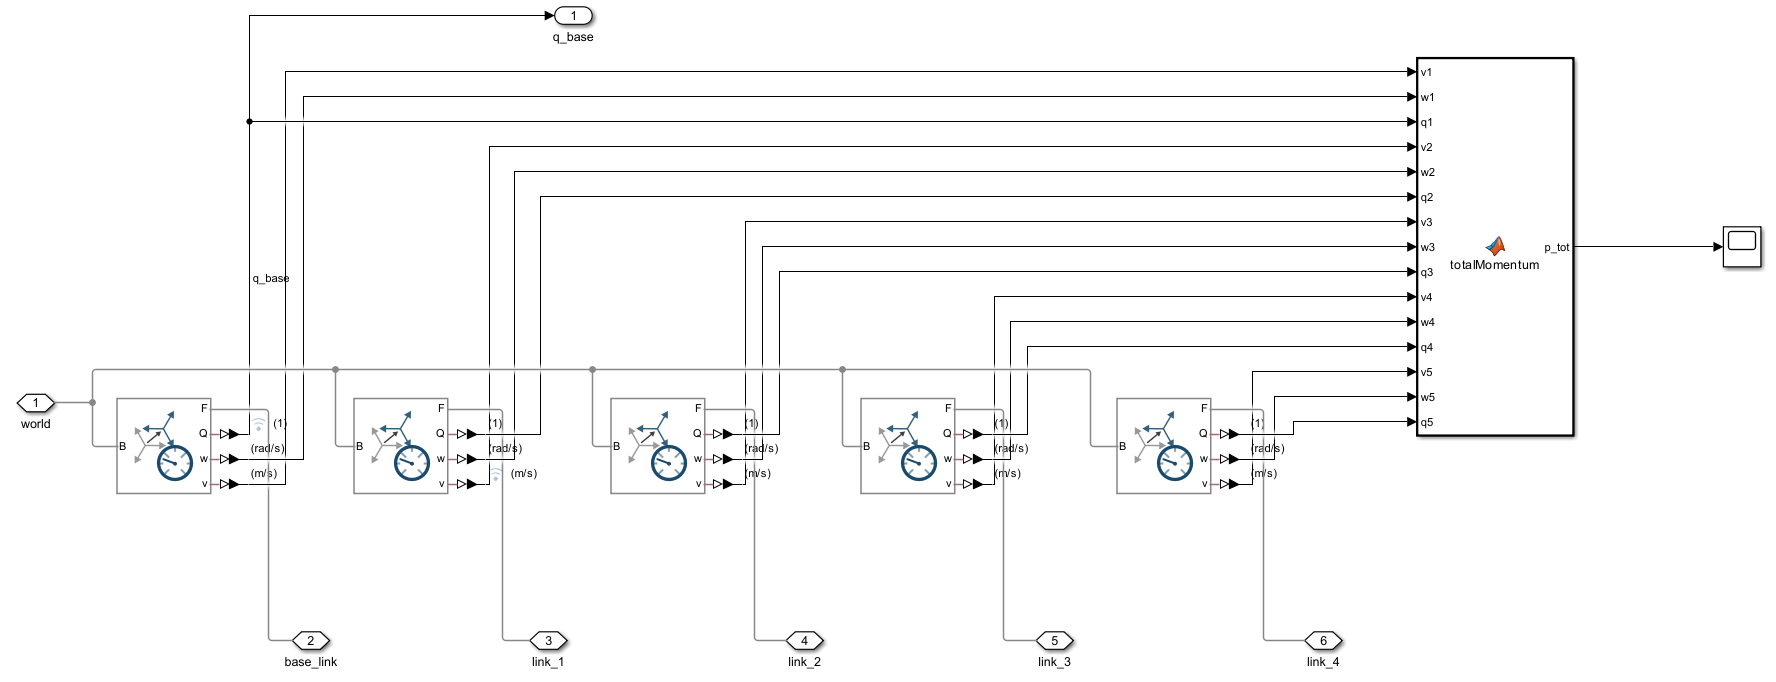
\includegraphics[width=1\linewidth]{Figures/impuls_monitor.png}
%DIFDELCMD <     %%%
\DIFdelendFL \DIFaddbeginFL 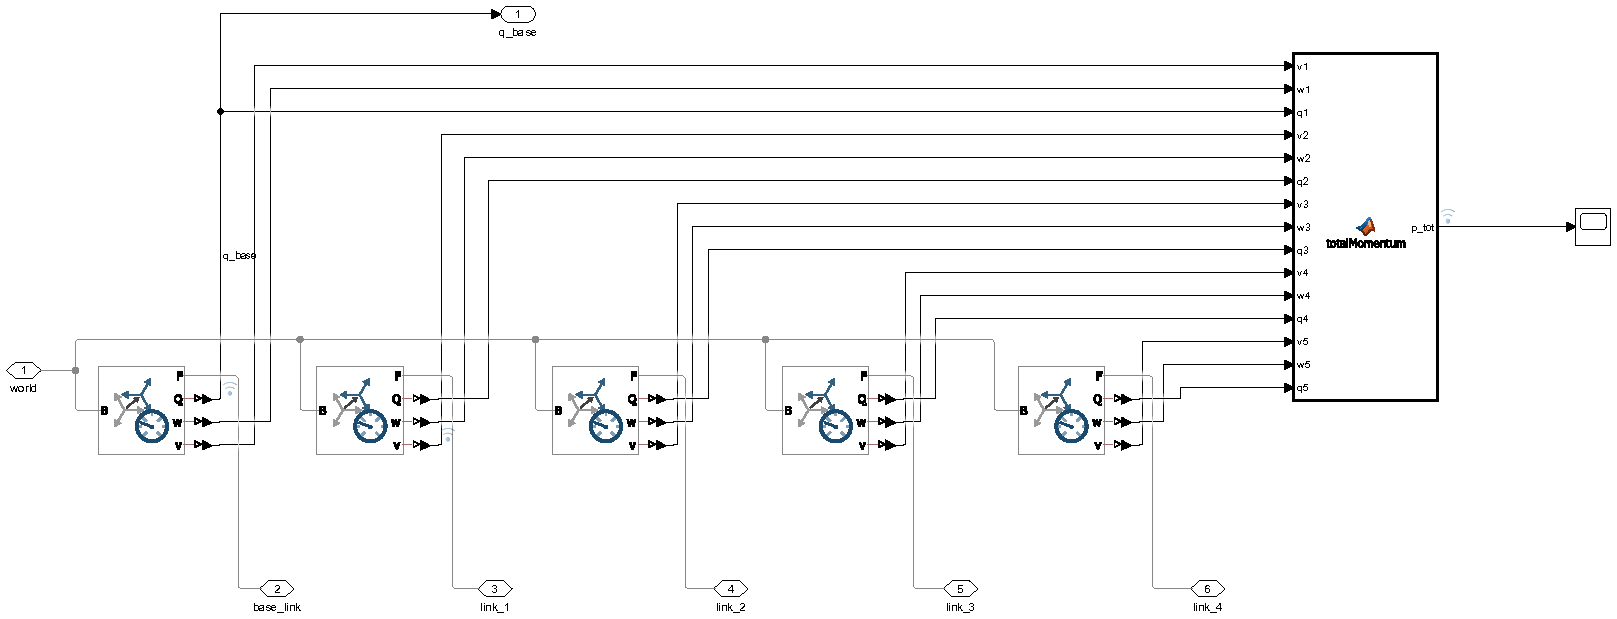
\includegraphics[width=1\linewidth]{Figures/impuls_monitor.pdf}
    \DIFaddendFL \caption{Overview of the \DIFdelbeginFL \DIFdelFL{Impuls }\DIFdelendFL \DIFaddbeginFL \DIFaddFL{Momentum }\DIFaddendFL Monitor Subsystem (Momentum Observer) in the Simulink Model \texttt{SpaceRobot.slx} \\
    This figure shows the computation of the total linear and angular momentum of the free-floating space robot. 
    The velocities and orientations of the base and all manipulator links are measured and aggregated within a 
    MATLAB function to obtain the system momentum. This monitor is used to analyze momentum conservation and 
    quantify base–manipulator dynamic coupling effects.}
    \label{fig:impuls_monitor}
\end{figure*}
\begin{figure}[!b]
  \centering
  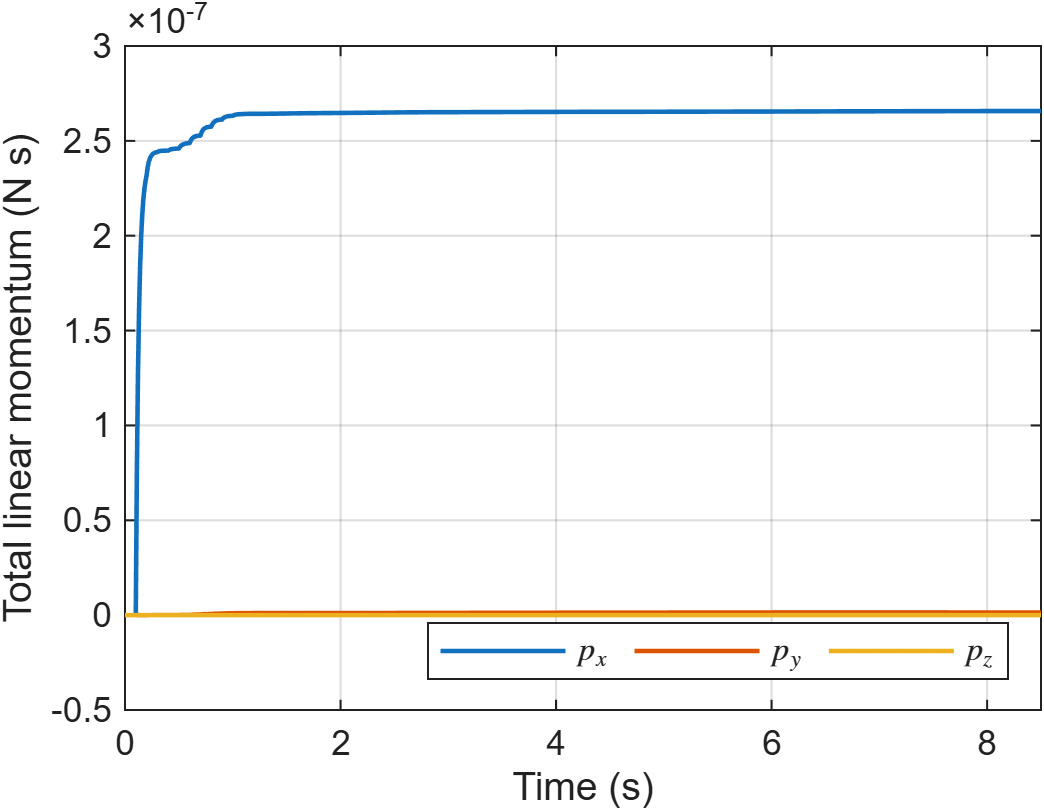
\includegraphics[width=0.95\linewidth]{Figures/impulserhaltung_scope.png}
  \caption{Dynamics of the total momentum of the robot.}
  \label{fig:impulserhaltung_scope}
\end{figure}
\noindent
\DIFdelbegin \DIFdel{Momentum Conservation Monitor: }\DIFdelend \DIFaddbegin \textbf{\DIFadd{Momentum Conservation Monitor.}} \DIFaddend In a free-floating system without external forces, \DIFaddbegin \DIFadd{both }\DIFaddend the total linear \DIFaddbegin \DIFadd{and the total angular }\DIFaddend momentum of the robot (base \DIFdelbegin \DIFdel{+ arm) should remain constant (and in our case, near zero since initial momentumis zero ) \mbox{%DIFAUXCMD
\cite{b6}}\hskip0pt%DIFAUXCMD
. We implemented a Momentum Observer that }\DIFdelend \DIFaddbegin \DIFadd{and arm) are conserved. With zero initial momentum, the total linear momentum remains close to zero throughout the simulation \mbox{%DIFAUXCMD
\cite{b6}}\hskip0pt%DIFAUXCMD
. A momentum observer }\DIFaddend continuously
computes the total linear momentum \DIFdelbegin \DIFdel{$p_{tot}$ of the system }\DIFdelend \DIFaddbegin \DIFadd{$p_{\mathrm{tot}}$ }\DIFaddend and checks for its conservation (see \Cref{fig:impuls_monitor}). \DIFdelbegin \DIFdel{This is done by attaching virtual sensors }\DIFdelend \DIFaddbegin \DIFadd{Virtual sensors attached to the base and }\DIFaddend to \DIFdelbegin \DIFdel{each body (base and links) to measure their velocitiesand computing $p_{tot} = \sum_{i} m_{i} v_{i}$}\DIFdelend \DIFaddbegin \DIFadd{each link provide the body velocities, from which $p_{\mathrm{tot}} = \sum_{i} m_{i} v_{i}$ is computed. The same observer aggregates the link velocities and orientations to track the total angular momentum, which is conserved as well}\DIFaddend . In an ideal simulation, \DIFdelbegin \DIFdel{$p_{tot}$ stays roughly zero at all times (small }\DIFdelend \DIFaddbegin \DIFadd{$p_{\mathrm{tot}}$ remains close to zero throughout an episode. Small }\DIFaddend numerical deviations on the order of \DIFdelbegin \DIFdel{$10^{-6}$ Ns may occur due to integration errors). If a significant, systematic change in
$p_{tot}$ were detected, it }\DIFdelend \DIFaddbegin \DIFadd{$10^{-6}\,\mathrm{Ns}$ may arise from time-integration errors. A persistent, systematic drift of $p_{\mathrm{tot}}$ }\DIFaddend would indicate an unintended external force or a modeling error\DIFdelbegin \DIFdel{(}\DIFdelend \DIFaddbegin \DIFadd{, }\DIFaddend such as an unmodeled constraint\DIFdelbegin \DIFdel{or bug). During our experiments, $p_{tot}$ remained near
$0$ (within $10^{-6}$ Ns) }\DIFdelend \DIFaddbegin \DIFadd{. In the reported experiments, $p_{\mathrm{tot}}$ remained within $10^{-6}\,\mathrm{Ns}$ of zero }\DIFaddend throughout each episode with the learned policy \DIFdelbegin \DIFdel{, confirming physical
consistency }\DIFdelend (see~\autoref{fig:impulserhaltung_scope})\DIFdelbegin \DIFdel{. This momentum check provides confidence that the simulation adheres to
Newton’s laws and the agent interacts with a physical correct process. This leverages the significance of the obtained policy. The Momentum Conservation 
Monitor }\DIFdelend \DIFaddbegin \DIFadd{, which confirms the physical consistency of the simulation. The momentum observer }\DIFaddend also serves as a diagnostic tool\DIFdelbegin \DIFdel{because }\DIFdelend \DIFaddbegin \DIFadd{, as }\DIFaddend any momentum drift would pause training for model inspection.

\begin{figure*}[!t]
    \centering    \DIFdelbeginFL %DIFDELCMD < 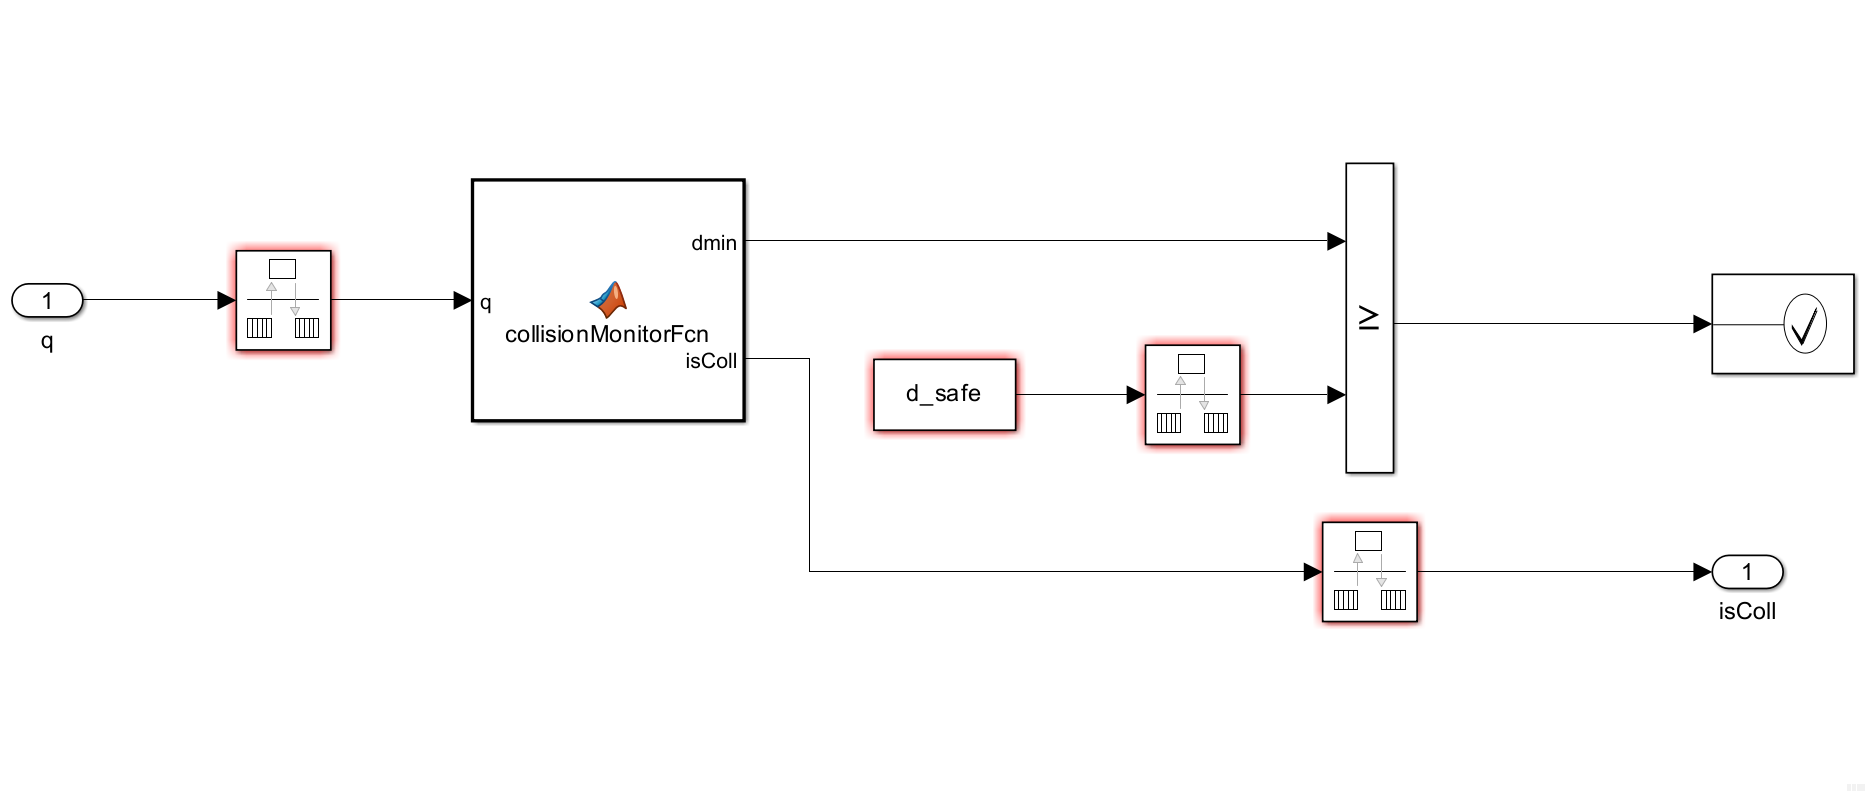
\includegraphics[width=0.75\linewidth]{Figures/spacerobot_slx_colissionmonitor.png}
%DIFDELCMD <     %%%
\DIFdelendFL \DIFaddbeginFL 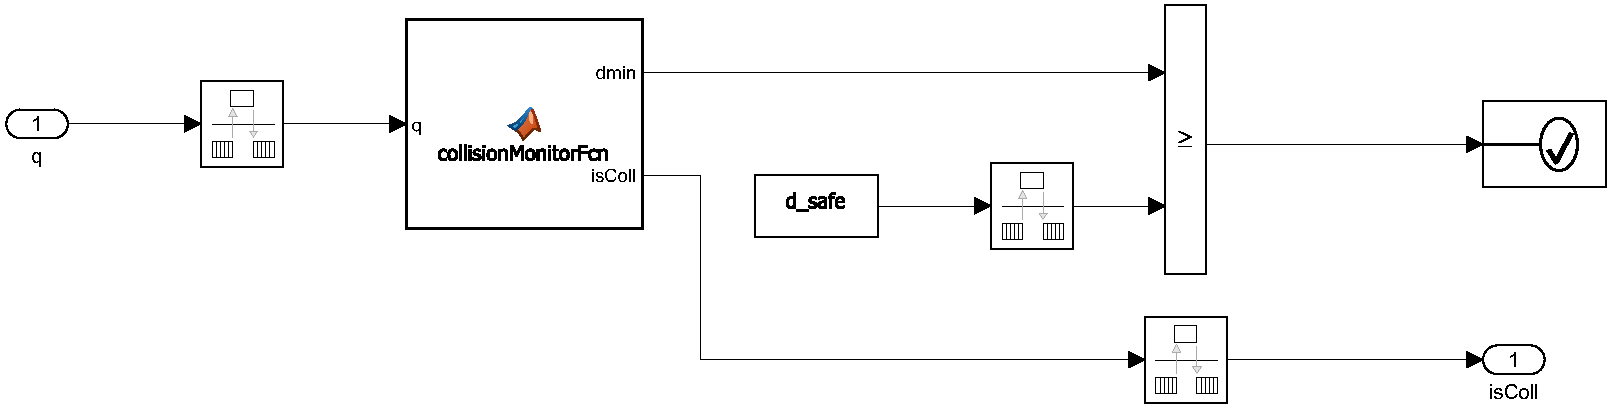
\includegraphics[width=0.75\linewidth]{Figures/spacerobot_slx_colissionmonitor.pdf}
    \DIFaddendFL \caption{Overview of the Collision Monitor Subsystem in the Simulink Model \texttt{SpaceRobot.slx} \\
    This figure illustrates the collision monitoring logic used to ensure safe robot operation during training and 
    evaluation. Joint and link configurations are processed to compute the minimum distance to obstacles, which is 
    compared against a predefined safety threshold. A collision flag is generated and used for episode termination 
    or safety-related penalties.}
    \label{fig:spacerobot_slx_colissionmonitor}
\end{figure*}

\begin{figure*}[!t] 
    \centering
    \begin{subfigure}[b]{0.48\textwidth}
        \centering
        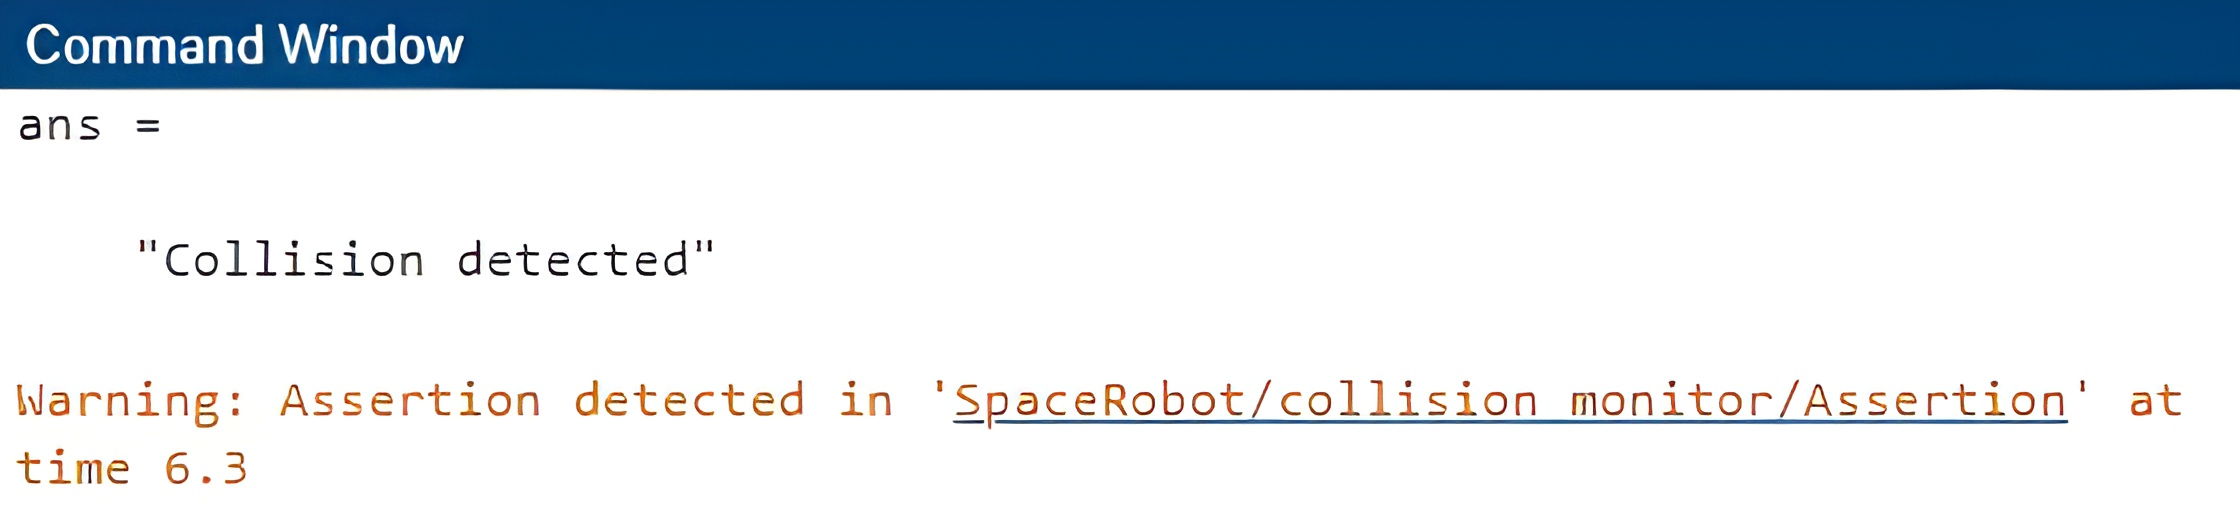
\includegraphics[width=\linewidth]{Figures/warning_collision.png}
        \caption{Automatically triggered collision warning}
        \label{fig:collision_warning}
    \end{subfigure}
    \hfill
    \begin{subfigure}[b]{0.48\textwidth}
        \centering
        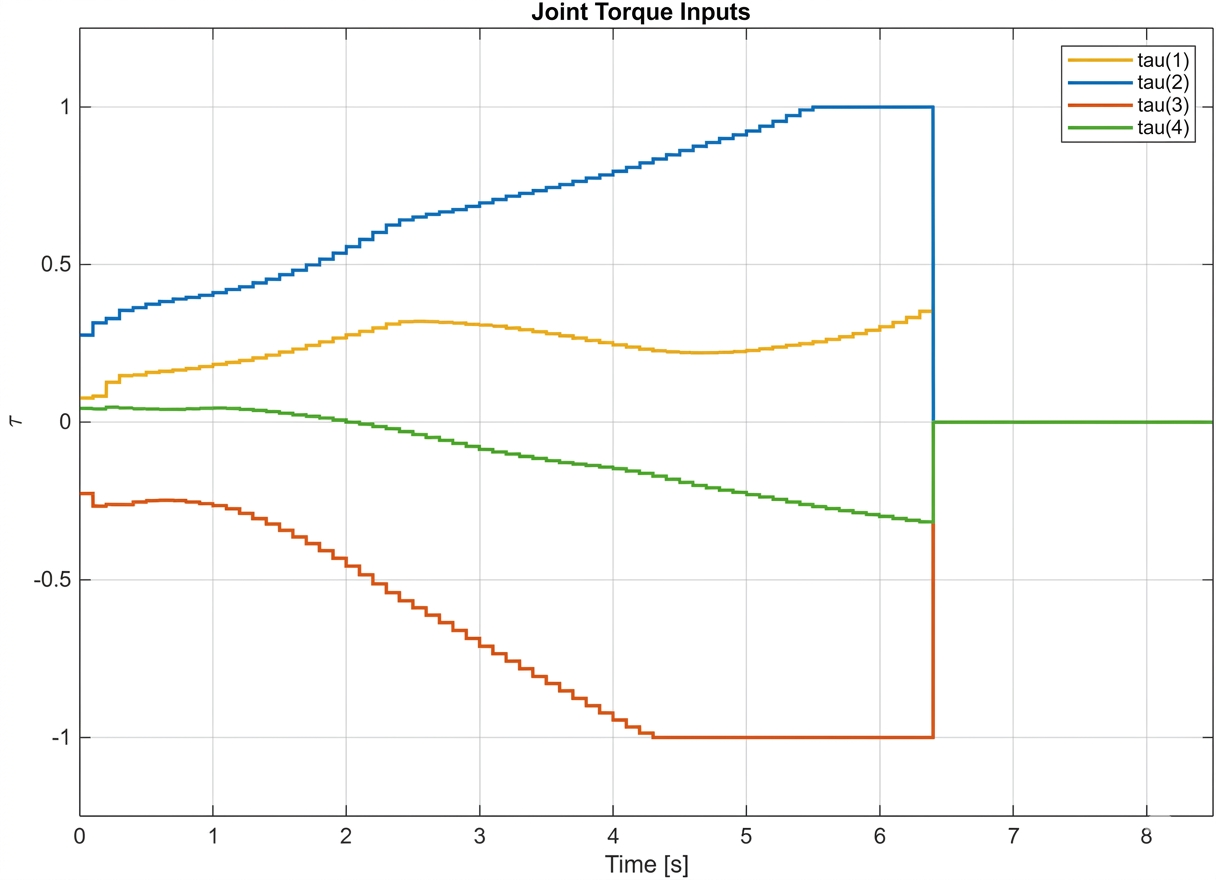
\includegraphics[width=\linewidth]{Figures/tau_collision.png}
        \caption{Scope of torque inputs in the event of a collision}
        \label{fig:collision_scope}
    \end{subfigure}
    \caption{Representation of collision detection and the associated torque curves.}
    \label{fig:collision_combined}
\end{figure*}
\noindent
\DIFdelbegin \DIFdel{Collision Monitor and Avoidance: We define a minimum allowable distance between certain
}\DIFdelend \DIFaddbegin \textbf{\DIFadd{Collision Monitor and Avoidance.}} \DIFadd{A minimum admissible distance is defined between selected
}\DIFaddend parts of the robot (\DIFdelbegin \DIFdel{for example, }\DIFdelend \DIFaddbegin \DIFadd{e.g.\ }\DIFaddend between the end-effector and the base structure). \DIFdelbegin \DIFdel{A Collision
Monitor subsystem computes distances between predefined pairs of bodies each step (using the geometry from the URDF and Simscape’s collision detection capabilities). If any distance falls
below the safe threshold $d_{safe}$ (indicating a potential collision or self-collision is
imminent), the system triggers }\DIFdelend \DIFaddbegin \DIFadd{At every time step, a collision monitor computes the distances between the predefined body pairs using the URDF geometry and the Simscape collision-detection facilities. When any distance drops below the safety threshold $d_{\mathrm{safe}}$, }\DIFaddend a collision event \DIFaddbegin \DIFadd{is triggered }\DIFaddend (see \Cref{fig:spacerobot_slx_colissionmonitor}) \cite{b31}. \DIFdelbegin \DIFdel{In our simulation, 
we set, e.g., $d_{safe} = 5$ cm as the minimum clearance. When triggered, the following occurs: (1)}\DIFdelend \DIFaddbegin \DIFadd{A value of $d_{\mathrm{safe}} = 5\,\mathrm{cm}$ is used in this work. Upon activation, three actions are performed, namely (i)~}\DIFaddend a warning flag is raised and logged\DIFdelbegin \DIFdel{(for analysis), (2)a done signal is sent to terminate the episodeimmediately}\DIFdelend , \DIFaddbegin \DIFadd{(ii)~a }\texttt{\DIFadd{done}} \DIFadd{signal terminates the episode, }\DIFaddend and (\DIFdelbegin \DIFdel{3)all joint torque commands from the agent }\DIFdelend \DIFaddbegin \DIFadd{iii)~all commanded joint torques }\DIFaddend are overridden to zero\DIFdelbegin \DIFdel{to stop the robotmotion. This mechanism 
effectively acts as an emergency brake, preventing the agent from
continuing once a collision is about to happen. The collision monitor was tested by deliberately
}\DIFdelend \DIFaddbegin \DIFadd{, stopping the robot. The monitor was verified by intentionally }\DIFaddend commanding the arm toward the base. It reliably detected the \DIFdelbegin \DIFdel{violation of the safety distance }\DIFdelend \DIFaddbegin \DIFadd{threshold violation }\DIFaddend and stopped the system (see~\autoref{fig:collision_combined}). During training\DIFdelbegin \DIFdel{of the RL agents}\DIFdelend , collisions occurred in early exploratory
episodes for some agents, but \DIFdelbegin \DIFdel{the monitor caught them and ended those episodes with heavy
penalties. As trainingprogressed}\DIFdelend \DIFaddbegin \DIFadd{were captured by the monitor and penalized through episode termination. By the end of training}\DIFaddend , all agents \DIFdelbegin \DIFdel{learned to avoid collisions altogether, indeed, }\DIFdelend \DIFaddbegin \DIFadd{avoided collisions }\DIFaddend in the final evaluation \DIFdelbegin \DIFdel{all agents achieved  episode without any collision ($K5 = 0$), confirming the efficacy of
this safety measure}\DIFdelend \DIFaddbegin \DIFadd{($K_5 = 0$ over all 30 evaluation episodes)}\DIFaddend .

\DIFdelbegin \DIFdel{Joint Limit Enforcement: The robot arm has joint angle limits (e.g., each revolute joint might be
limited to ±180° or a smaller range based on mechanical constraints). Violating joint }\DIFdelend \DIFaddbegin \textbf{\DIFadd{Joint Limit Enforcement.}} \DIFadd{Each revolute joint of the arm is subject to mechanical limits. Violating these }\DIFaddend limits could damage a real robot and \DIFdelbegin \DIFdel{often }\DIFdelend \DIFaddbegin \DIFadd{typically }\DIFaddend indicates an unstable controller. \DIFdelbegin \DIFdel{We enforce joint limits }\DIFdelend \DIFaddbegin \DIFadd{The joint limits are enforced }\DIFaddend at two levels. First, \DIFdelbegin \DIFdel{in }\DIFdelend the Simscape model \DIFdelbegin \DIFdel{, we include }\DIFdelend \DIFaddbegin \DIFadd{includes }\DIFaddend mechanical joint limits with penalty forces\DIFdelbegin \DIFdel{(}\DIFdelend \DIFaddbegin \DIFadd{, i.e.\ }\DIFaddend a stiff barrier that \DIFdelbegin \DIFdel{resists }\DIFdelend \DIFaddbegin \DIFadd{opposes }\DIFaddend further motion beyond the limit\DIFdelbegin \DIFdel{)}\DIFdelend . Second, \DIFdelbegin \DIFdel{we add an Assertion block that
}\DIFdelend \DIFaddbegin \DIFadd{an assertion block }\DIFaddend monitors each joint angle. If any joint exceeds its \DIFdelbegin \DIFdel{predefined limit}\DIFdelend \DIFaddbegin \DIFadd{admissible range}\DIFaddend , the assertion triggers a violation event \DIFdelbegin \DIFdel{. Similarly to the collision case, we handle a joint limit violation by: terminating
the episode, applying a large negative }\DIFdelend \DIFaddbegin \DIFadd{that terminates the episode, applies a negative terminal }\DIFaddend reward, and \DIFdelbegin \DIFdel{zeroing out all torques immediately. In
fact, the Simulink model is configured such that when the assertion triggers, it directly sets the
torque inputs $\tau$ to zero in that }\DIFdelend \DIFaddbegin \DIFadd{sets all torques to zero within the }\DIFaddend same time step\DIFdelbegin \DIFdel{as a protective measure. This ensures the
robot doesn’t push further }\DIFdelend \DIFaddbegin \DIFadd{. This prevents further motion }\DIFaddend into the limit\DIFdelbegin \DIFdel{or oscillate. In our results, we observed very few limit
violations once agents were trained. Among all algorithms, }\DIFdelend \DIFaddbegin \DIFadd{. After training, the joint-limit violation rate is low. }\DIFaddend PPO and TRPO \DIFdelbegin \DIFdel{had a handful of
episodes grazing the limits (K6 values of }\DIFdelend \DIFaddbegin \DIFadd{reach the limits in }\DIFaddend a few percent \DIFaddbegin \DIFadd{of evaluation steps (5.1\% and 2.1\%, respectively}\DIFaddend ), whereas TD3, SAC, PG, and DDPG \DIFdelbegin \DIFdel{essentially never hit the limits ($K6 \approx 0$). Notably, PPO ’s superior tracking performance came
at the cost of occasionally using the full joint range (K6 = 0.0505, i.e.~\textasciitilde5\% of episodes, had minor
limit violations). Thanks to the joint limit enforcement , these events did not lead to
instability: the agent’s torques were cut off momentarily when a limit was reached, preventing
any damaging behavior, }\DIFdelend \DIFaddbegin \DIFadd{remain within the admissible range ($K_6 \approx 0$). The higher $K_6$ value of PPO ($K_6 = 0.0505$) coincides with the lowest tracking error and indicates a more aggressive use of the workspace. In all cases, the enforcement mechanism stopped further simulated motion at the limit. The torques were set to zero in the offending step }\DIFaddend and the episode was marked as failed. \DIFdelbegin \DIFdel{Over time, the agent learned to
avoid this scenario as well, especially in the optimized PPO version (where K6 dropped to 0}\DIFdelend \DIFaddbegin \DIFadd{For the optimized PPO agent (}\autoref{sec:reward_ablation}\DIFadd{), no such events are observed in the evaluation episodes ($K_6 = 0$}\DIFaddend ).

\DIFdelbegin %DIFDELCMD < \noindent
%DIFDELCMD < %%%
\DIFdel{Formal Verification of Torque Constraints: }\DIFdelend \DIFaddbegin \textbf{\DIFadd{Formal Verification of Torque Constraints.}} \DIFaddend In addition to \DIFdelbegin \DIFdel{enforcing torque saturationduring
simulation, we performed }\DIFdelend \DIFaddbegin \DIFadd{runtime saturation, }\DIFaddend an offline formal verification \DIFdelbegin \DIFdel{to prove that }\DIFdelend \DIFaddbegin \DIFadd{was performed to check torque-bound compliance of }\DIFaddend the trained policy \DIFdelbegin \DIFdel{could
not command out-of-bounds torques}\DIFdelend \DIFaddbegin \DIFadd{block}\DIFaddend . Using MATLAB \DIFdelbegin \DIFdel{’s }\DIFdelend Simulink Design Verifier (SLDV) in property-proving mode,
\DIFdelbegin \DIFdel{we analyzed }\DIFdelend a simplified closed-loop model of the agent \DIFdelbegin \DIFdel{controlling the robot’s
joints}\DIFdelend \DIFaddbegin \DIFadd{and the joint torques was analyzed}\DIFaddend . The property to \DIFdelbegin \DIFdel{prove was thatfor all possible agent inputs (observations), each output }\DIFdelend \DIFaddbegin \DIFadd{be checked is that, for any admissible observation input in the analyzed abstraction, each commanded }\DIFaddend torque $\tau_i$ \DIFdelbegin \DIFdel{remains within }%DIFDELCMD < [%%%
\DIFdel{$-\tau_{\max}$, $+\tau_{\max}$}%DIFDELCMD < ] %%%
\DIFdelend \DIFaddbegin \DIFadd{satisfies $\tau_i \in [-\tau_{\max}, +\tau_{\max}]$ }\DIFaddend (see \Cref{fig:verify_tau}). \DIFdelbegin \DIFdel{The
verification succeeded: SLDV was able to prove that no counterexample exists and the torque
limits are always respected by the policy network. ~}\DIFdelend \DIFaddbegin \DIFadd{SLDV found no counterexample for this property. The corresponding SLDV result is shown in }\DIFaddend \autoref{fig:verify_tau_result} \DIFdelbegin \DIFdel{shows the SLDV result confirming the property (no violations found) }\DIFdelend \cite{b5}. This \DIFdelbegin \DIFdel{formal assurance is important because it
considers all possible states, including ones not seen during simulation, and guarantees the
policy cannot output a dangerous torque. It’s worth noting that directly running formal analysis
on }\DIFdelend \DIFaddbegin \DIFadd{result applies to the simplified verification model, including admissible abstract states not visited during simulation. Note that }\DIFaddend the full Simscape model \DIFdelbegin \DIFdel{was not feasible, }\DIFdelend \DIFaddbegin \DIFadd{is not amenable to property proving because of }\DIFaddend the nonlinear dynamics\DIFdelbegin \DIFdel{are too complex for the
automated theorem proving. To circumvent this, we extracted the relevant part of the model (the
control law and saturation logic) into a separate }\DIFdelend \DIFaddbegin \DIFadd{. The verification was performed on a }\DIFaddend simplified model (\DIFdelbegin \DIFdel{Verify\_tau.slx) where
}\DIFdelend \DIFaddbegin \texttt{\DIFadd{Verify\_tau.slx}}\DIFadd{) in which }\DIFaddend the plant was replaced by a worst-case abstraction\DIFdelbegin \DIFdel{(essentially, we just needed to check }\DIFdelend \DIFaddbegin \DIFadd{, because only }\DIFaddend the policy output block \DIFdelbegin \DIFdel{). This exemplifies }\DIFdelend \DIFaddbegin \DIFadd{is relevant for the considered property. This illustrates }\DIFaddend how formal methods can complement simulation-based learning \DIFdelbegin \DIFdel{: 
by verifying critical }\DIFdelend \DIFaddbegin \DIFadd{by checking selected }\DIFaddend properties on an abstract\DIFaddbegin \DIFadd{ed}\DIFaddend  model of the agent\DIFdelbegin \DIFdel{, we gain
additional confidence in safety beyond empirical testing}\DIFdelend .

\begin{figure}[!b]
	\centering    
	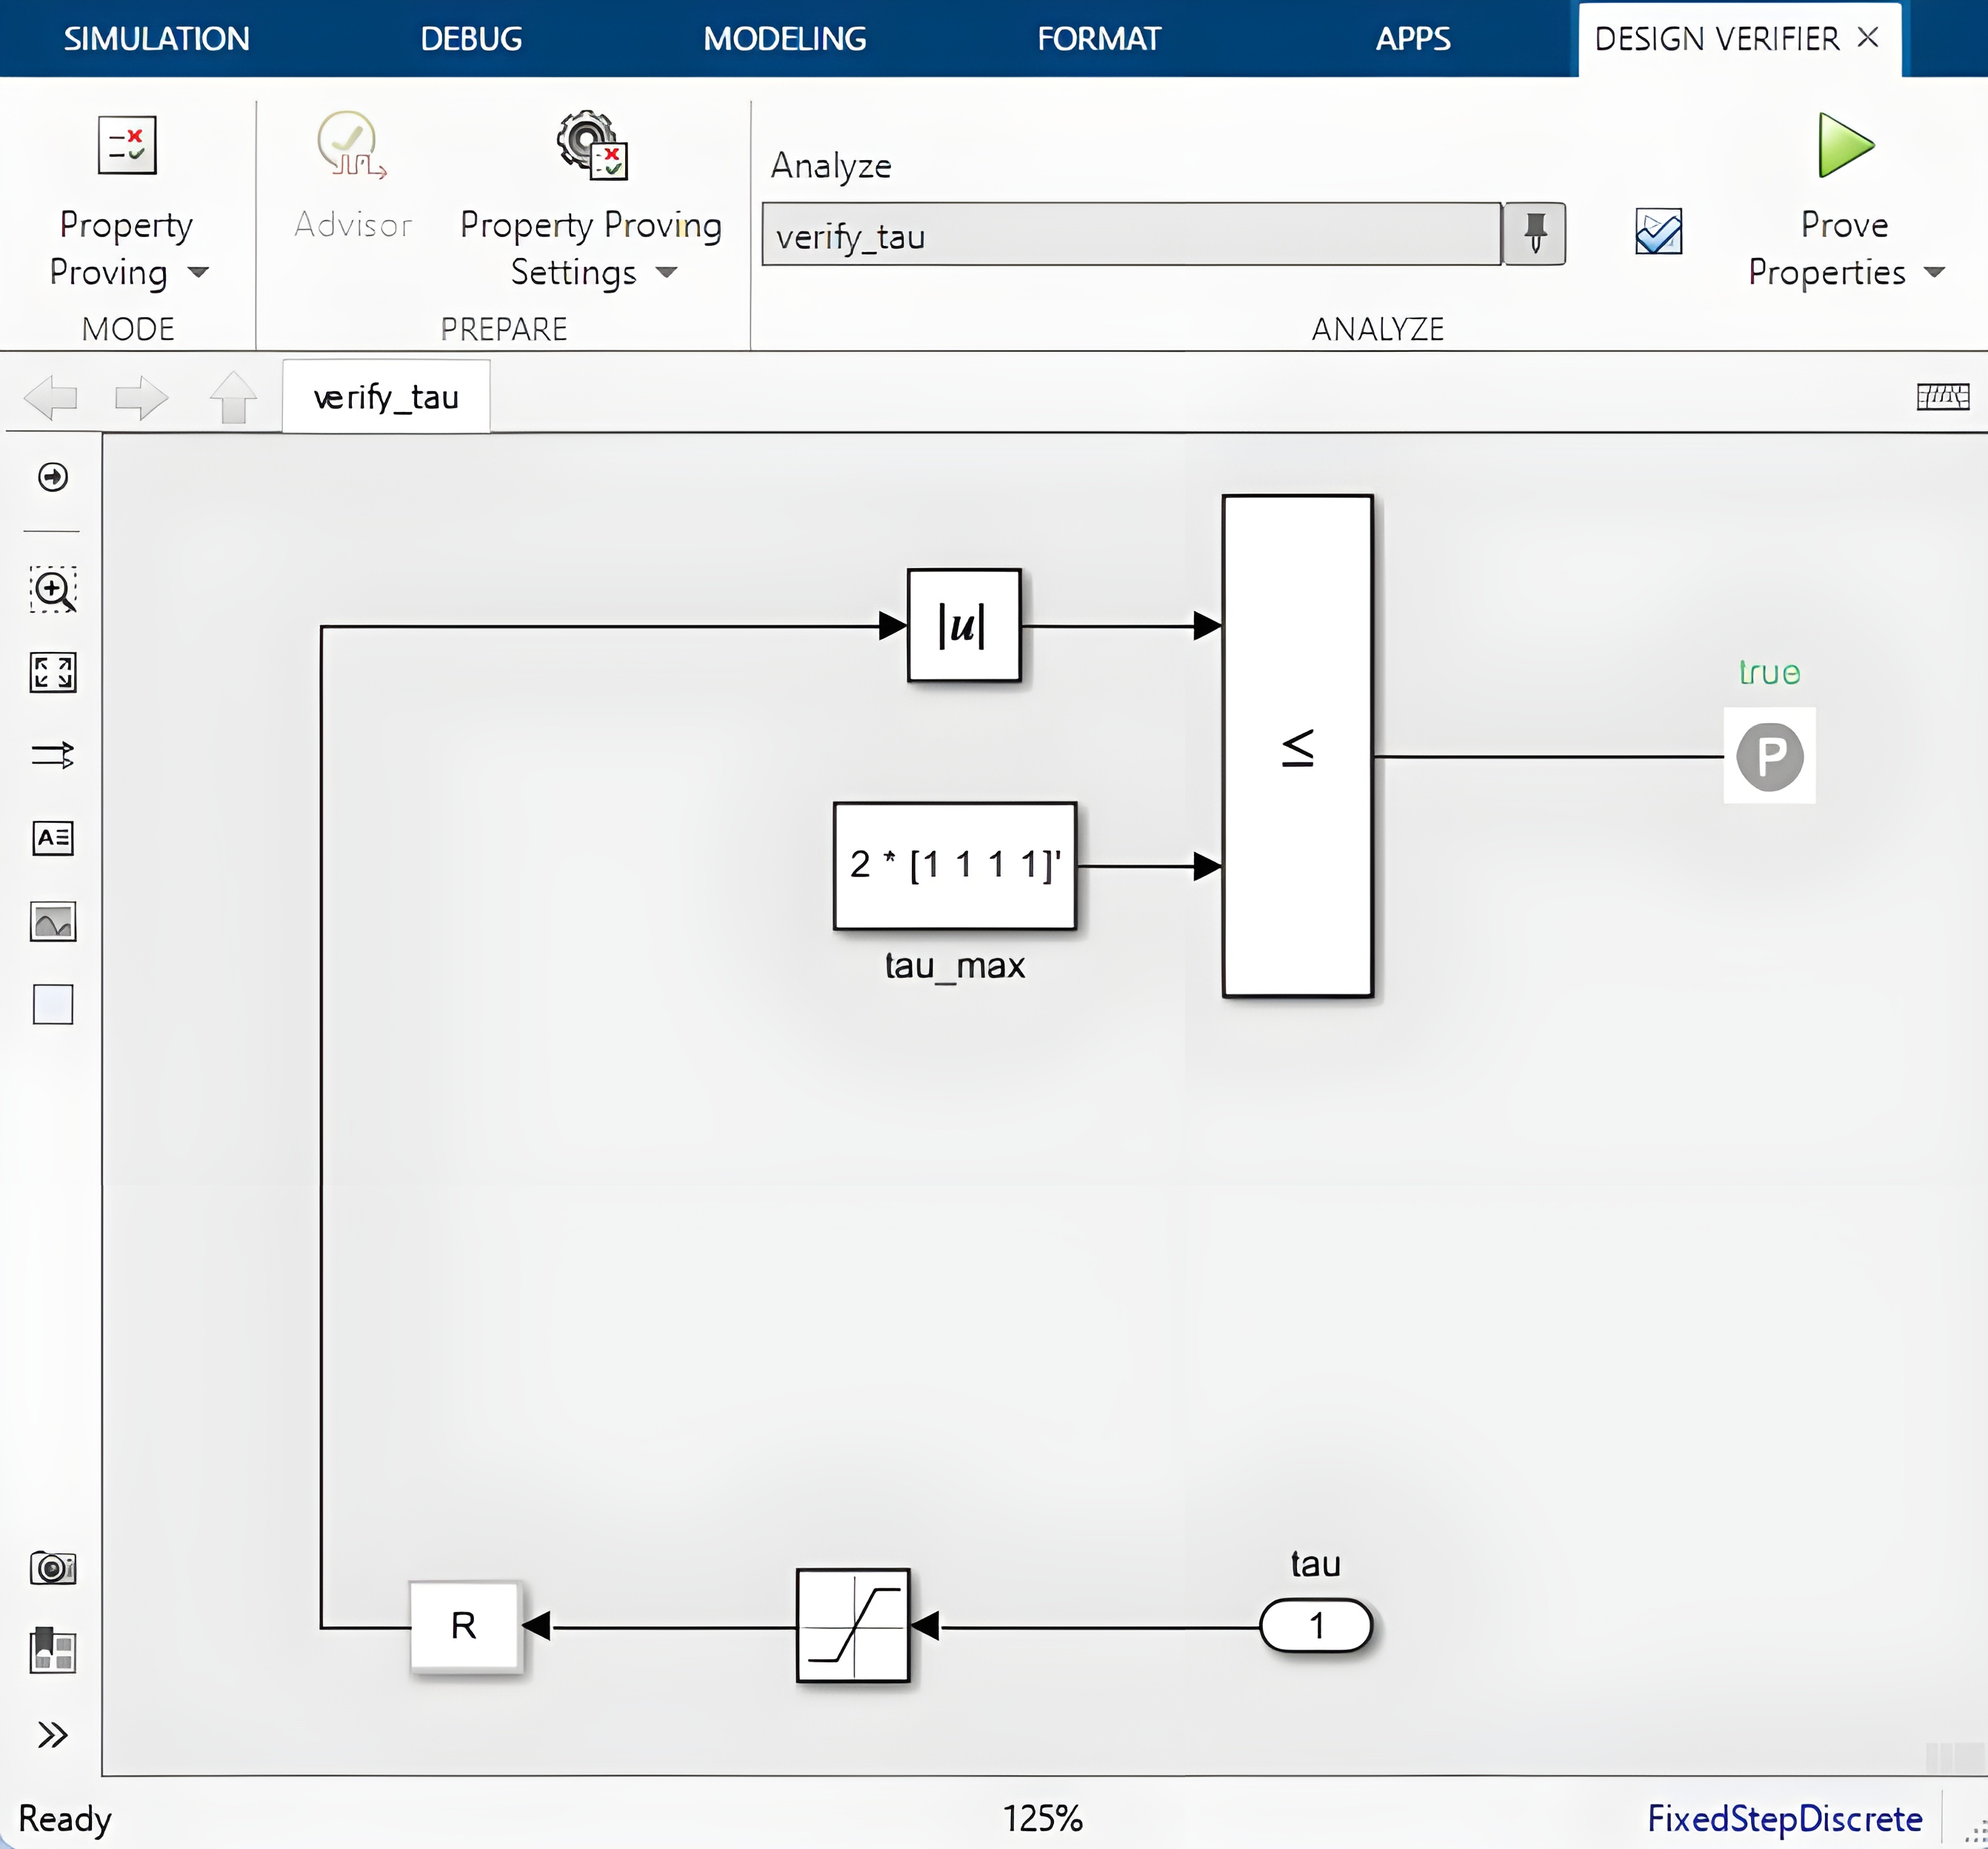
\includegraphics[width=\linewidth]{Figures/verify_tau_slx.png}
	\caption{Verification model with Simulink Design Verifier \texttt{Verify\_tau.slx} \\
  This figure depicts the Simulink property model used to formally verify the joint torque constraints. 
  The absolute joint torques are compared against predefined maximum limits using a relational operator. 
  The property is \DIFdelbeginFL \DIFdelFL{proven to hold for all reachable system states}\DIFdelendFL \DIFaddbeginFL \DIFaddFL{checked over the analyzed abstract state space}\DIFaddendFL , \DIFdelbeginFL \DIFdelFL{ensuring }\DIFdelendFL \DIFaddbeginFL \DIFaddFL{supporting }\DIFaddendFL bounded control actions \DIFaddbeginFL \DIFaddFL{in the verification model}\DIFaddendFL .}
	\label{fig:verify_tau}
\end{figure}

\DIFdelbegin \DIFdel{Limitations of Formal Methods: While the above components significantly enhance safety, we
observe that they cover a limited set of properties. They ensure zero collisions, no joint position overshot, and }\DIFdelend \DIFaddbegin \textbf{\DIFadd{Limitations of the Formal Methods Component.}} \DIFadd{The mechanisms above cover a defined set of monitored properties, namely collision events, joint-limit events, }\DIFaddend bounded torques, and \DIFdelbegin \DIFdel{they monitor physical consistency (e.g., momentum ). However, other aspects, such as guaranteeing }\DIFdelend \DIFaddbegin \DIFadd{physical consistency through the momentum check. Other properties, such as }\DIFaddend task completion within a time \DIFdelbegin \DIFdel{or }\DIFdelend \DIFaddbegin \DIFadd{bound or formal }\DIFaddend stability margins, \DIFdelbegin \DIFdel{were not formally }\DIFdelend \DIFaddbegin \DIFadd{are not }\DIFaddend verified. A complete formal specification of the \DIFdelbegin \DIFdel{entire mission(for instance, something like
temporal logic specifications of “}\DIFdelend \DIFaddbegin \DIFadd{mission, for example temporal-logic specifications such as ``}\DIFaddend the robot shall accomplish \DIFdelbegin \DIFdel{X without Y happening”) would be far }\DIFdelend \DIFaddbegin \DIFadd{$X$ without $Y$ happening'', would be substantially }\DIFaddend more complex. \DIFdelbegin \DIFdel{Our approach selectively targets the most critical safety concerns. In practice, this proved
sufficient to train successful policies without a single catastrophic failure: }\DIFdelend \DIFaddbegin \DIFadd{The present work targets the safety properties that are most relevant for the considered task. Within this scope, the runtime monitors terminated }\DIFaddend episodes that would have \DIFdelbegin \DIFdel{been catastrophic were safely stopped by the monitors (and heavily penalized to teach the agent). As a
result, by }\DIFdelend \DIFaddbegin \DIFadd{violated a monitored property and penalized }\DIFaddend the \DIFaddbegin \DIFadd{corresponding actions. By the }\DIFaddend end of training, the \DIFdelbegin \DIFdel{learned agent’s behavior was entirely meaningful }\DIFdelend \DIFaddbegin \DIFadd{policy operated }\DIFaddend within the safety envelope \DIFdelbegin \DIFdel{enforced by the formal constraints }\DIFdelend \DIFaddbegin \DIFadd{defined by the monitored constraints in the reported evaluation episodes }\DIFaddend \cite{b23}.

In summary, \DIFdelbegin \DIFdel{integrating these }\DIFdelend \DIFaddbegin \DIFadd{the }\DIFaddend formal safety checks \DIFaddbegin \DIFadd{integrated }\DIFaddend into the learning process \DIFdelbegin \DIFdel{was vital. It not only
protected the simulation (and a potential future real system) from damage }\DIFdelend \DIFaddbegin \DIFadd{helped prevent unsafe simulated states }\DIFaddend during the exploratory phase of \DIFdelbegin \DIFdel{learning, but it also }\DIFdelend \DIFaddbegin \DIFadd{training and }\DIFaddend shaped the agent\DIFdelbegin \DIFdel{’}\DIFdelend \DIFaddbegin \DIFadd{'}\DIFaddend s behavior by penalizing unsafe actions. The agent \DIFdelbegin \DIFdel{thus
}\DIFdelend \DIFaddbegin \DIFadd{therefore }\DIFaddend learns with a \DIFdelbegin \DIFdel{form of built-in “}\DIFdelend \DIFaddbegin \DIFadd{runtime }\DIFaddend safety shield. \DIFdelbegin \DIFdel{” This approach demonstrates a viable path to apply }\DIFdelend \DIFaddbegin \DIFadd{This combination of monitored runtime constraints and penalty-driven learning is one approach to deploying }\DIFaddend deep RL in safety-critical domains \DIFdelbegin \DIFdel{like }\DIFdelend \DIFaddbegin \DIFadd{such as }\DIFaddend space robotics, \DIFdelbegin \DIFdel{where pure }\DIFdelend \DIFaddbegin \DIFadd{in which unconstrained }\DIFaddend trial-and-error \DIFdelbegin \DIFdel{without safeguards would be
unacceptable. We next analyze the performance outcomes of the various }\DIFdelend \DIFaddbegin \DIFadd{exploration is not admissible. The next section analyzes the performance of the six }\DIFaddend RL agents under these conditions.
\DIFaddbegin 

\textbf{\DIFadd{Computational Overhead and Scalability.}} \DIFadd{The three safety monitors, namely the momentum observer, collision distance checker, and joint-limit assertion, each consist of simple algebraic operations over the robot's link states, scaling as $\mathcal{O}(n_{\text{links}})$ per time step. For the 4-DOF arm considered here, this overhead is negligible compared to the physics simulation itself. End-to-end training times, including the full safety stack, are reported as metric $T_3$ in }\autoref{tab:kpi_comp}\DIFadd{. They range from approximately 8 minutes (PG, PPO) to 38 minutes (TD3) for 1000 episodes on a standard workstation (AMD Ryzen 7 7700, 32 GB RAM). For onboard deployment, only the learned policy network needs to execute in the control loop. The default PPO baseline uses a compact two-hidden-layer network (128 units per layer, $\approx$\,20\,000 parameters), while the optimized PPO configuration adopted for the final results (cf.\ \mbox{%DIFAUXCMD
\cref{sec:reward_ablation}}\hskip0pt%DIFAUXCMD
) uses a deeper $[256, 256, 128]$ policy with $\approx$\,1.05$\,\times\,10^{5}$ parameters, still on the order of $10^5$ weights and well below the memory footprint of typical perception networks deployed on space-qualified hardware. At the 10\,Hz control rate used here, a single forward pass through this network requires on the order of $2\,\times\,10^{5}$ multiply-accumulate operations per step, which is compatible with the throughput of modern space-qualified embedded processors (e.g., ARM Cortex-A or LEON-class CPUs with a hardware FPU). The safety monitors can be retained as lightweight parallel watchdog processes, or reduced to the most safety-critical checks (torque saturation, joint-limit assertion) with minimal additional compute. This modular architecture supports scalability to resource-constrained onboard systems.
}

\DIFaddend \begin{figure}[!b]
	\centering
	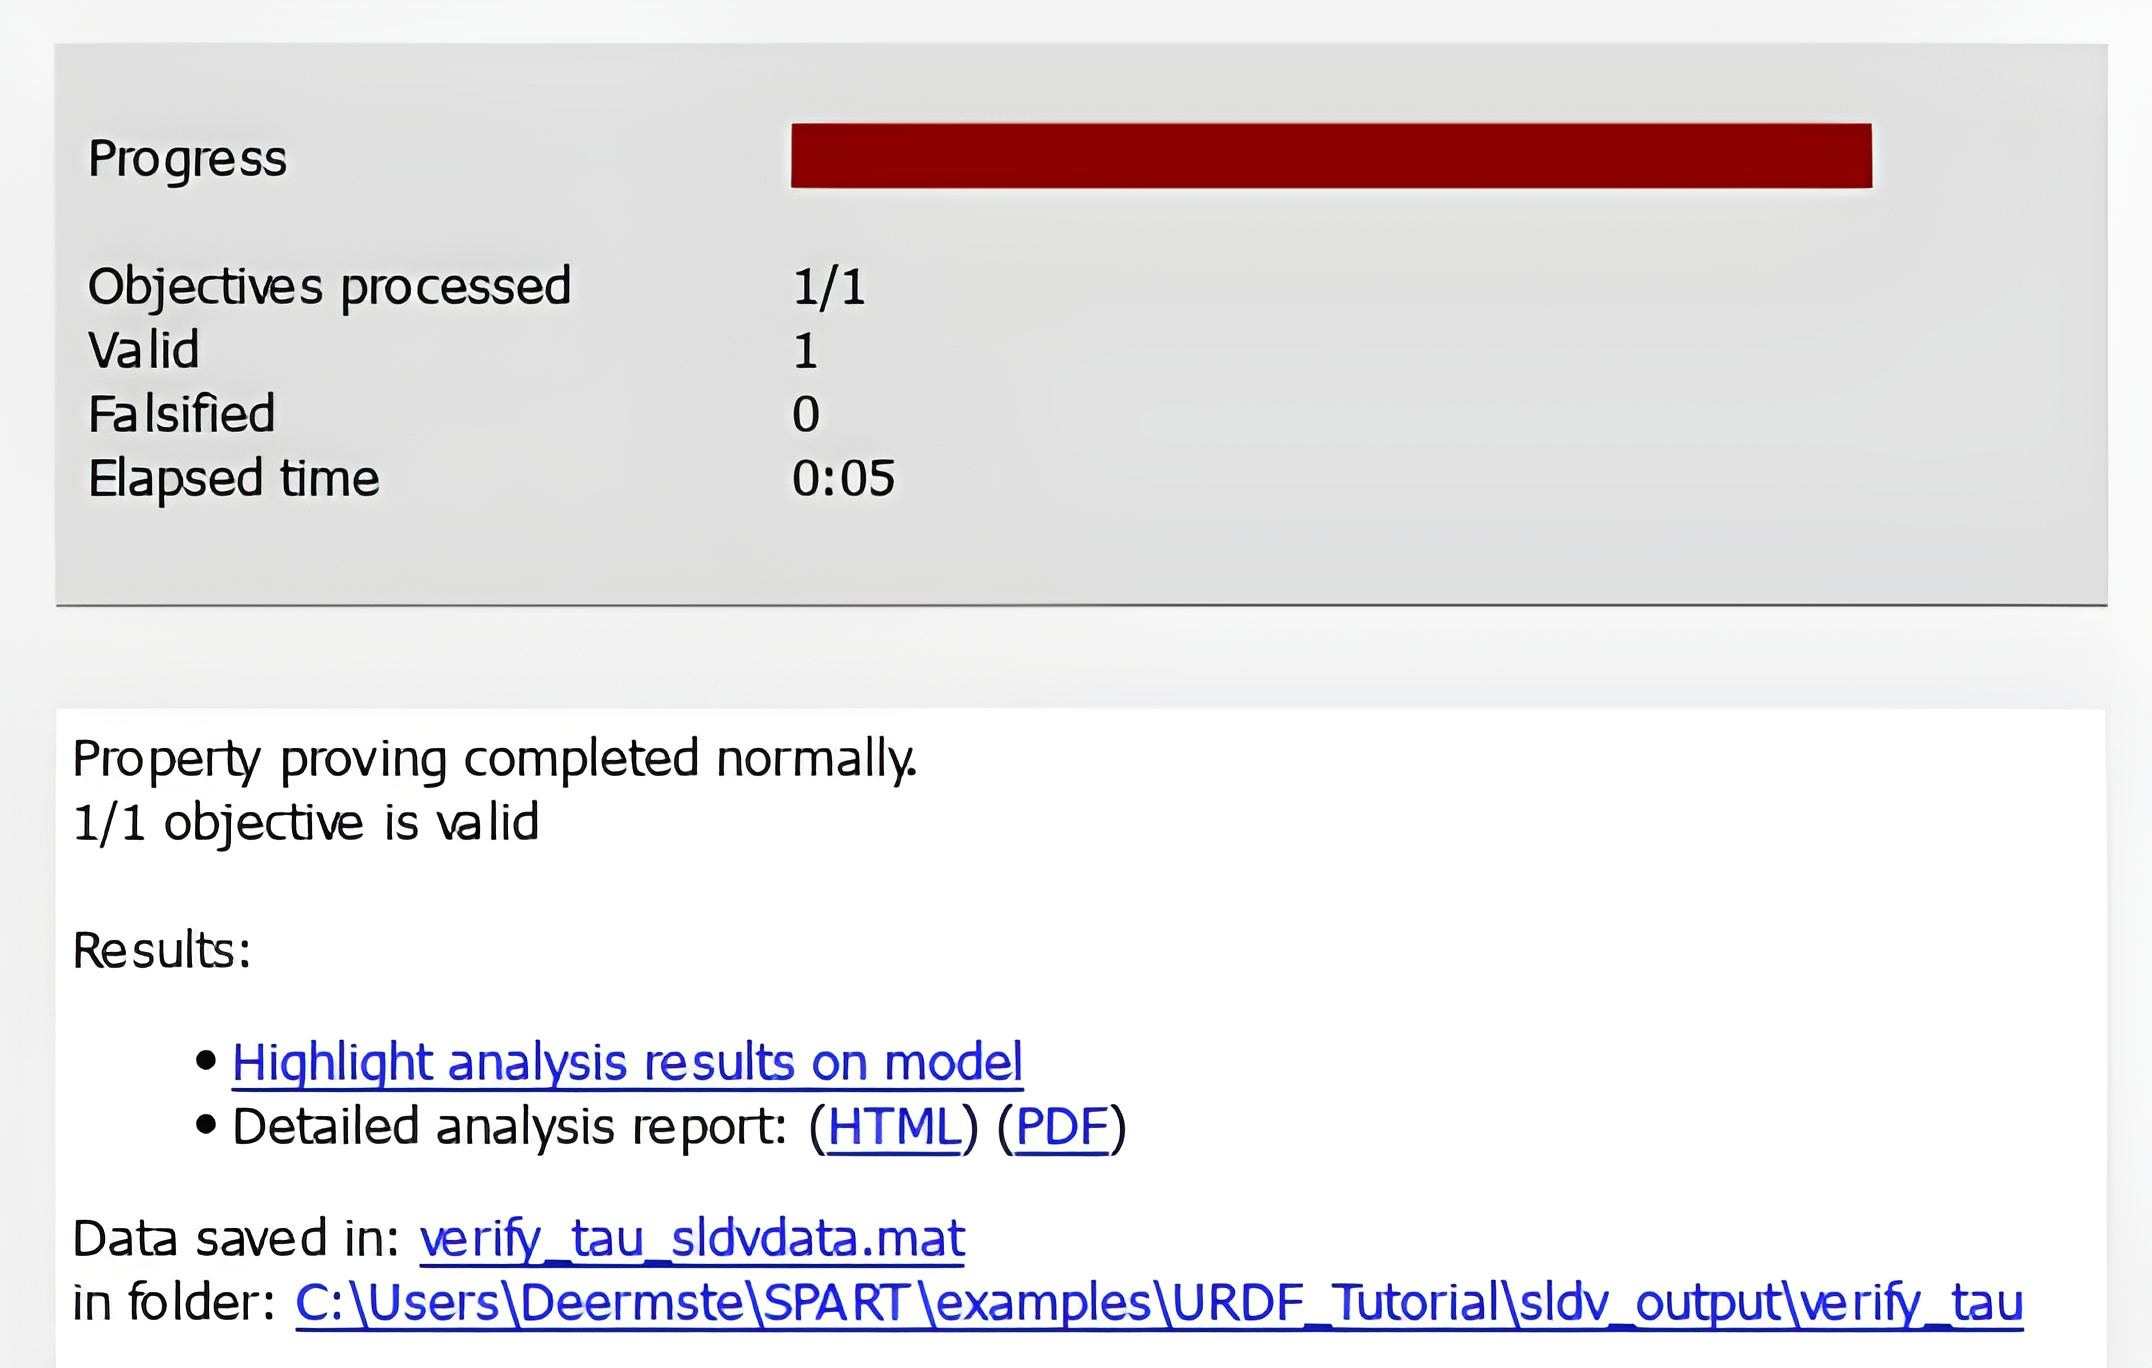
\includegraphics[width=\linewidth]{Figures/verify_tau_reslult.png}
	\caption{Result of the Simulink Design Verifier \\ 
  This figure shows the result of a formal property verification performed on the torque constraint model. 
  The verification confirms that the specified safety property is satisfied for all analyzed execution paths. 
  This analysis provides \DIFdelbeginFL \DIFdelFL{formal guarantees on control torque limits }\DIFdelendFL \DIFaddbeginFL \DIFaddFL{model-based evidence for torque-limit compliance }\DIFaddendFL beyond empirical simulation-based validation.}
	\label{fig:verify_tau_result}
\end{figure}

\section{Comparison of Continuous RL Agents} \label{comparison}
\DIFdelbegin \DIFdel{A central question of this study is: Which }\DIFdelend \DIFaddbegin \DIFadd{This section compares six }\DIFaddend continuous-action RL \DIFdelbegin \DIFdel{algorithm is most effective for
controlling a free-floating space robot? To answer this, we evaluated six RL }\DIFdelend algorithms from three \DIFdelbegin \DIFdel{major
}\DIFdelend families on the same task and environment \cite{b2,b7}. The algorithms \DIFdelbegin \DIFdel{compared }\DIFdelend \DIFaddbegin \DIFadd{considered }\DIFaddend are:

\begin{itemize}
  \item \DIFdelbegin \DIFdel{Policy Gradient (PG): the classic }\DIFdelend \DIFaddbegin \textit{\DIFadd{Policy Gradient (PG).}} \DIFadd{The }\DIFaddend REINFORCE algorithm (Monte Carlo policy gradient), included as
a baseline for direct policy optimization without \DIFdelbegin \DIFdel{advanced variance reduction }\DIFdelend \DIFaddbegin \DIFadd{variance-reduction techniques }\DIFaddend \cite{b7,b21}.
  \item \DIFdelbegin \DIFdel{Proximal Policy Optimization (PPO): a modern }\DIFdelend \DIFaddbegin \textit{\DIFadd{Proximal Policy Optimization (PPO).}} \DIFadd{A }\DIFaddend policy-gradient method that uses \DIFdelbegin \DIFdel{clipped
probability ratio updates to ensure stable and conservative policy improvements. PPO is known
for its balance of stability and performance }\DIFdelend \DIFaddbegin \DIFadd{a clipped
probability-ratio surrogate to bound policy updates }\DIFaddend \cite{b15}.
  \item \DIFdelbegin \DIFdel{Trust Region Policy Optimization (TRPO): a }\DIFdelend \DIFaddbegin \textit{\DIFadd{Trust Region Policy Optimization (TRPO).}} \DIFadd{A }\DIFaddend policy-gradient method that enforces a trust-region
constraint \DIFdelbegin \DIFdel{(via Kullback–Leibler divergence) on policy updates. TRPO is expected to perform similarly to
PPO in terms of stability, albeit with higher computational cost due to solving a constrained
optimization each update }\DIFdelend \DIFaddbegin \DIFadd{based on the Kullback--Leibler divergence at each update. The constrained optimization step incurs a higher per-update computational cost than PPO }\DIFaddend \cite{b14}.
  \item \DIFdelbegin \DIFdel{Deep Deterministic Policy Gradient (DDPG): an }\DIFdelend \DIFaddbegin \textit{\DIFadd{Deep Deterministic Policy Gradient (DDPG).}} \DIFadd{An }\DIFaddend off-policy actor-critic algorithm with a
deterministic policy and target networks. DDPG \DIFdelbegin \DIFdel{can excel in continuous control by learning a Q-function 
}\DIFdelend \DIFaddbegin \DIFadd{jointly learns a $Q$-function }\DIFaddend and a policy \DIFdelbegin \DIFdel{simultaneously, but it is known to be sensitive to hyperparameters and can
be unstable }\DIFdelend \DIFaddbegin \DIFadd{and is sensitive to hyperparameter choices }\DIFaddend \cite{b16}.
  \item \DIFdelbegin \DIFdel{Twin Delayed DDPG (TD3): an improved }\DIFdelend \DIFaddbegin \textit{\DIFadd{Twin Delayed DDPG (TD3).}} \DIFadd{A }\DIFaddend variant of DDPG that \DIFdelbegin \DIFdel{addresses function approximation
issues by using }\DIFdelend \DIFaddbegin \DIFadd{uses }\DIFaddend two critic networks to \DIFdelbegin \DIFdel{mitigate }\DIFdelend \DIFaddbegin \DIFadd{reduce }\DIFaddend overestimation bias and \DIFdelbegin \DIFdel{by delaying policy updates . TD3 generally offers more stable learning than standard DDPG }\DIFdelend \DIFaddbegin \DIFadd{delays policy updates relative to value updates }\DIFaddend \cite{b17}.
  \item \DIFdelbegin \DIFdel{Soft Actor-Critic (SAC): an }\DIFdelend \DIFaddbegin \textit{\DIFadd{Soft Actor-Critic (SAC).}} \DIFadd{An }\DIFaddend off-policy actor-critic algorithm \DIFdelbegin \DIFdel{that learns }\DIFdelend \DIFaddbegin \DIFadd{with }\DIFaddend a stochastic policy and \DIFdelbegin \DIFdel{includes }\DIFdelend an entropy term in the \DIFdelbegin \DIFdel{reward to encourage exploration. SAC aims to achieve both
high reward and high entropy , making the agent’s behavior robust and exploratory. It often
achieves very good performance but can be computationally heavier due to sampling and
entropy calculations }\DIFdelend \DIFaddbegin \DIFadd{objective. This entropy regularization promotes exploration but increases the per-step computational cost relative to deterministic methods }\DIFaddend \cite{b18}.
\end{itemize}
\DIFdelbegin \DIFdel{These algorithms cover a spectrum from }\DIFdelend \DIFaddbegin 

\DIFadd{The six algorithms cover the }\DIFaddend on-policy\DIFdelbegin \DIFdel{to }\DIFdelend \DIFaddbegin \DIFadd{/}\DIFaddend off-policy \DIFdelbegin \DIFdel{, from deterministicto stochastic , and
from simpler to more complex }\DIFdelend \DIFaddbegin \DIFadd{and deterministic/stochastic axes, as well as a range of }\DIFaddend update rules. \DIFdelbegin \DIFdel{Based on prior knowledge and the nature of our problem, we hypothesized that algorithms with more robust, stable }\DIFdelend \DIFaddbegin \DIFadd{Given the strong base--manipulator coupling and the safety constraints, methods with constrained or clipped }\DIFaddend policy updates (\DIFdelbegin \DIFdel{like PPOand TRPO) would
likely outperform others in this highly coupled, continuous control scenario. Off-policy }\DIFdelend \DIFaddbegin \DIFadd{PPO, TRPO) are expected to provide more stable training than algorithms without such constraints (PG, DDPG). The off-policy actor-critic }\DIFaddend methods (DDPG, TD3, SAC) \DIFdelbegin \DIFdel{might reach good performance as well, but could suffer from tuning sensitivity and
stability issues given the complex dynamics and safety constraints. Indeed, DDPG and basic PG were
expected to be the least reliable due to known tendencies for instability without additional
regularization}\DIFdelend \DIFaddbegin \DIFadd{may achieve comparable performance but are typically more sensitive to hyperparameter selection}\DIFaddend .

\begin{table}[!t]
\centering
\caption{Classification of the evaluated reinforcement learning algorithms.}
\label{tab:on_off_policy}
\begin{tabular}{ll}
\toprule
\textbf{Algorithm} & \textbf{Policy Type} \\
\midrule
Policy Gradient (PG) & On-policy \\
Proximal Policy Optimization (PPO) & On-policy  \\
Trust Region Policy Optimization (TRPO) & On-policy  \\
Deep Deterministic Policy Gradient (DDPG) & Off-policy  \\
Twin Delayed DDPG (TD3) & Off-policy  \\
Soft Actor-Critic (SAC) & Off-policy  \\
\bottomrule
\end{tabular}
\end{table}
On-policy methods (PG, PPO, TRPO) update \DIFdelbegin \DIFdel{their policies using only data from }\DIFdelend \DIFaddbegin \DIFadd{the policy only from data generated by }\DIFaddend the current policy, \DIFdelbegin \DIFdel{leading }\DIFdelend \DIFaddbegin \DIFadd{which typically leads }\DIFaddend to stable but less sample-efficient learning. Off-policy methods (DDPG, TD3, SAC) reuse experience \DIFdelbegin \DIFdel{from }\DIFdelend \DIFaddbegin \DIFadd{stored in }\DIFaddend a replay buffer, \DIFdelbegin \DIFdel{improving }\DIFdelend \DIFaddbegin \DIFadd{which improves }\DIFaddend sample efficiency at the cost of higher sensitivity to hyperparameters~\cite{b2,b7}. For free-floating \DIFdelbegin \DIFdel{space 
robot control , where }\DIFdelend \DIFaddbegin \DIFadd{space-robot control with }\DIFaddend strong nonlinear coupling and safety constraints\DIFdelbegin \DIFdel{demand reliable convergence, }\DIFdelend \DIFaddbegin \DIFadd{, the constrained-update }\DIFaddend on-policy methods are expected to \DIFdelbegin \DIFdel{be advantageous}\DIFdelend \DIFaddbegin \DIFadd{provide more reliable convergence}\DIFaddend .

\textbf{Training Setup\DIFdelbegin \DIFdel{:}\DIFdelend \DIFaddbegin \DIFadd{.}\DIFaddend } All experiments were \DIFdelbegin \DIFdel{conducted }\DIFdelend \DIFaddbegin \DIFadd{performed }\DIFaddend on a workstation \DIFdelbegin \DIFdel{equipped }\DIFdelend with an AMD Ryzen 7 7700 processor and 32\DIFaddbegin \DIFadd{\,}\DIFaddend GB of RAM, using MATLAB R2025b with the Reinforcement Learning Toolbox and Simscape Multibody. \DIFdelbegin \DIFdel{We used the }\DIFdelend \DIFaddbegin \DIFadd{The }\DIFaddend same network architecture (\DIFdelbegin \DIFdel{initially }\DIFdelend two hidden layers of 128 units each for \DIFdelbegin \DIFdel{policy and for value function}\DIFdelend \DIFaddbegin \DIFadd{the policy and}\DIFaddend , where applicable\DIFdelbegin \DIFdel{) and same reward structure for all . Hyperparameters (learning rate, discount factor }\DIFdelend \DIFaddbegin \DIFadd{, for the value function) and the same reward function were used for all agents. The discount factor was fixed at }\DIFaddend $\gamma = 0.99$\DIFdelbegin \DIFdel{, etc. ) were initially set to default reasonable values and kept consistent across agents as
much as possible. All agents were trained using a learning rate of $\alpha = 1 \times 10^{-3}$ }\DIFdelend \DIFaddbegin \DIFadd{. The learning rate }\DIFaddend for both actor and critic networks \DIFdelbegin \DIFdel{, }\DIFdelend \DIFaddbegin \DIFadd{was $\alpha = 1 \times 10^{-3}$ }\DIFaddend unless stated otherwise. \DIFdelbegin \DIFdel{Hence, any }\DIFdelend \DIFaddbegin \DIFadd{With these unified settings, observed }\DIFaddend performance differences can be attributed primarily to the algorithmic differences \DIFdelbegin \DIFdel{, not }\DIFdelend \DIFaddbegin \DIFadd{rather than }\DIFaddend to unequal tuning. \DIFdelbegin \DIFdel{Later we will tune PPO further, but for }\DIFdelend \DIFaddbegin \DIFadd{PPO was further tuned in a subsequent step. In }\DIFaddend the main comparison, PPO uses \DIFdelbegin \DIFdel{a default configurationas well}\DIFdelend \DIFaddbegin \DIFadd{its default configuration}\DIFaddend . Each agent \DIFdelbegin \DIFdel{’s training
run of }\DIFdelend \DIFaddbegin \DIFadd{was trained for }\DIFaddend 1000 episodes\DIFdelbegin \DIFdel{yielded a final policy which we }\DIFdelend \DIFaddbegin \DIFadd{, and the resulting policy was }\DIFaddend then evaluated.

\textbf{Performance Metrics\DIFdelbegin \DIFdel{:}\DIFdelend \DIFaddbegin \DIFadd{.}\DIFaddend } \DIFdelbegin \DIFdel{We evaluated the agents }\DIFdelend \DIFaddbegin \DIFadd{The agents were evaluated }\DIFaddend on the KPIs \DIFdelbegin \DIFdel{described earlier (tracking error, base
stability, etc.) }\DIFdelend \DIFaddbegin \DIFadd{introduced in Section~\ref{RL} }\DIFaddend by running 30 \DIFdelbegin \DIFdel{test episodes for each. ~}\DIFdelend \DIFaddbegin \DIFadd{evaluation episodes per agent. }\DIFaddend \autoref{tab:kpi_comp} \DIFdelbegin \DIFdel{summarizes }\DIFdelend \DIFaddbegin \DIFadd{reports }\DIFaddend a subset of these metrics \DIFdelbegin \DIFdel{,
highlighting the differences between }\DIFdelend \DIFaddbegin \DIFadd{for the six }\DIFaddend agents.

\begin{table*}[!t]
\centering
\caption{Selected performance metrics for each RL agent (best \DIFdelbeginFL \DIFdelFL{values }\DIFdelendFL \DIFaddbeginFL \DIFaddFL{value }\DIFaddendFL in \DIFaddbeginFL \DIFaddFL{each row in }\DIFaddendFL bold). PPO \DIFdelbeginFL \DIFdelFL{excels in most
categories, achieving }\DIFdelendFL \DIFaddbeginFL \DIFaddFL{attains }\DIFaddendFL the
lowest tracking errors (K2, K3), \DIFdelbeginFL \DIFdelFL{best base stability }\DIFdelendFL \DIFaddbeginFL \DIFaddFL{the lowest base-orientation error }\DIFaddendFL (K4), and \DIFdelbeginFL \DIFdelFL{smoothest control
}\DIFdelendFL \DIFaddbeginFL \DIFaddFL{the lowest jerk }\DIFaddendFL (K7), \DIFdelbeginFL \DIFdelFL{while maintaining short }\DIFdelendFL \DIFaddbeginFL \DIFaddFL{with the
shortest }\DIFaddendFL training time \DIFaddbeginFL \DIFaddFL{(T3)}\DIFaddendFL . TRPO is \DIFdelbeginFL \DIFdelFL{a }\DIFdelendFL close \DIFdelbeginFL \DIFdelFL{second in many }\DIFdelendFL \DIFaddbeginFL \DIFaddFL{to PPO on several }\DIFaddendFL metrics but requires more training time. \DIFdelbeginFL \DIFdelFL{Off-policy }\DIFdelendFL \DIFaddbeginFL \DIFaddFL{The
off-policy }\DIFaddendFL methods (TD3, SAC, DDPG) show larger errors or \DIFdelbeginFL \DIFdelFL{instabilities }\DIFdelendFL \DIFaddbeginFL \DIFaddFL{a larger late-training reward variance }\DIFaddendFL (e.g., high
T1 for DDPG)\DIFdelbeginFL \DIFdelFL{despite some strengths (}\DIFdelendFL \DIFaddbeginFL \DIFaddFL{. }\DIFaddendFL DDPG \DIFdelbeginFL \DIFdelFL{'s low max }\DIFdelendFL \DIFaddbeginFL \DIFaddFL{attains the lowest maximum }\DIFaddendFL error \DIFaddbeginFL \DIFaddFL{(}\DIFaddendFL K3). \DIFdelbeginFL \DIFdelFL{KPI data from evaluation of }\DIFdelendFL \DIFaddbeginFL \DIFaddFL{Values are averaged over }\DIFaddendFL 30 \DIFaddbeginFL \DIFaddFL{evaluation }\DIFaddendFL episodes per agent.}
\label{tab:kpi_comp}
\renewcommand{\arraystretch}{1.3}
\setlength{\tabcolsep}{8pt}
\begin{tabular}{lcccccc}
\toprule
\textbf{KPI (unit)} & \textbf{TRPO} & \textbf{TD3} & \textbf{SAC} & \textbf{PPO} & \textbf{PG} & \textbf{DDPG} \\
\midrule
\textbf{K2:} Mean Squared EE position error &
0.0680 & 0.1914 & 0.1908 & \textbf{0.0257} & 0.1638 & 0.0937 \\
\textbf{K3:} Max EE error &
0.6783 & 0.5341 & 0.7766 & 0.4833 & 1.0654 & \textbf{0.4758} \\
\textbf{K4:} Mean base orientation error &
0.0694 & 0.0868 & 0.1687 & \textbf{0.0667} & 0.1302 & 0.2682 \\
\textbf{K6:} Joint limit violation rate &
0.0214 (2.1\%) & 0 & 0 & 0.0505 (5.1\%) & 0 & 0 \\
\textbf{K7:} Torque smoothness (norm.\ jerk) &
0.7498 & 0.9981 & 0.7536 & \textbf{0.6812} & 0.7125 & 0.8118 \\
\textbf{T1:} Reward std.\ (late training) &
\textbf{0.6144} & 8.5168 & 9.6907 & 1.7756 & 13.1970 & 64.4764 \\
\textbf{T3:} Training time (1000 eps) &
$\sim$13\,min & $\sim$38\,min & $\sim$35\,min & \textbf{$\sim$8\,min} & $\sim$8\,min & $\sim$24\,min \\
\bottomrule
\end{tabular}
\end{table*}

\DIFdelbegin %DIFDELCMD < \noindent
%DIFDELCMD < %%%
\DIFdelend The results in \autoref{tab:kpi_comp} \DIFdelbegin \DIFdel{reveal clear patterns across the six agents. Regarding }\DIFdelend \DIFaddbegin \DIFadd{display the following patterns. With respect to }\DIFaddend \emph{training stability}, TRPO and PPO \DIFdelbegin \DIFdel{exhibited the most stable learning (T1 values of 0.61 and 1.78}\DIFdelend \DIFaddbegin \DIFadd{yield the smallest late-training reward variance ($T_1 = 0.61$ and $T_1 = 1.78$}\DIFaddend , respectively), whereas DDPG \DIFdelbegin \DIFdel{showed highly 
erratic behavior (T1\,=\,64.5). PPO was also the fastest to train (T3\,$\approx$\,8\,min), while }\DIFdelend \DIFaddbegin \DIFadd{shows the largest ($T_1 = 64.5$). The training time $T_3$ is shortest for PPO ($\approx 8\,\mathrm{min}$). The }\DIFaddend off-policy methods \DIFdelbegin \DIFdel{required substantially longer }\DIFdelend \DIFaddbegin \DIFadd{are slower }\DIFaddend (TD3 \DIFdelbegin \DIFdel{\,$\approx$\,38\,min, SAC \,$\approx$\,35\,min}\DIFdelend \DIFaddbegin \DIFadd{$\approx 38\,\mathrm{min}$, SAC $\approx 35\,\mathrm{min}$}\DIFaddend ).

\DIFdelbegin \DIFdel{In terms of }\DIFdelend \DIFaddbegin \DIFadd{For }\DIFaddend \emph{trajectory tracking}, PPO \DIFdelbegin \DIFdel{achieved }\DIFdelend \DIFaddbegin \DIFadd{attains }\DIFaddend the lowest mean squared error (\DIFdelbegin \DIFdel{K2\,=\,0.0257), significantly 
outperforming the runner-up TRPO (0.0680}\DIFdelend \DIFaddbegin \DIFadd{$K_2 = 0.0257$), lower than that of TRPO ($K_2 = 0.0680$}\DIFaddend ). DDPG \DIFdelbegin \DIFdel{achieved }\DIFdelend \DIFaddbegin \DIFadd{attains }\DIFaddend the lowest peak error (\DIFdelbegin \DIFdel{K3\,=\,0.4758) in its best runs 
but was highly inconsistent}\DIFdelend \DIFaddbegin \DIFadd{$K_3 = 0.4758$) but with large variability across runs}\DIFaddend . PG, SAC, and TD3 \DIFdelbegin \DIFdel{all exhibited substantially }\DIFdelend \DIFaddbegin \DIFadd{yield }\DIFaddend larger tracking errors\DIFdelbegin \DIFdel{, with PG's mean error roughly }\DIFdelend \DIFaddbegin \DIFadd{. The mean error of PG is approximately }\DIFaddend six times that of PPO.

For \emph{\DIFdelbegin \DIFdel{base motion }\DIFdelend \DIFaddbegin \DIFadd{base-motion }\DIFaddend minimization}, PPO and TRPO \DIFdelbegin \DIFdel{both kept the base orientation error small (K4 of 0.0667 and 0.0694}\DIFdelend \DIFaddbegin \DIFadd{yield comparable base-orientation errors ($K_4 = 0.0667$ and $K_4 = 0.0694$}\DIFaddend ), while DDPG \DIFdelbegin \DIFdel{allowed the base to drift considerably (K4\,=\,0.2682). Interestingly, }\DIFdelend \DIFaddbegin \DIFadd{produces a larger drift ($K_4 = 0.2682$). }\DIFaddend TD3 \DIFdelbegin \DIFdel{achieved very }\DIFdelend \DIFaddbegin \DIFadd{yields a }\DIFaddend low base angular velocity (\DIFdelbegin \DIFdel{K8\,$\approx$\,0.02\,rad/s) by adopting an overly conservative strategy that sacrificed tracking accuracy}\DIFdelend \DIFaddbegin \DIFadd{$K_8 \approx 0.02\,\mathrm{rad/s}$) at the cost of degraded tracking accuracy, consistent with a conservative policy that suppresses actuation}\DIFaddend . All agents \DIFdelbegin \DIFdel{successfully avoided collisions (K5\,=\,0}\DIFdelend \DIFaddbegin \DIFadd{avoid collisions ($K_5 = 0$}\DIFaddend ). PPO and TRPO \DIFdelbegin \DIFdel{occasionally approached joint limits (K6 of 5.1\% and 2.1\%}\DIFdelend \DIFaddbegin \DIFadd{approach the joint limits in a small fraction of the steps ($K_6 = 5.1\%$ and $K_6 = 2.1\%$}\DIFaddend , respectively), \DIFdelbegin \DIFdel{indicating more aggressive }\DIFdelend \DIFaddbegin \DIFadd{corresponding to a wider }\DIFaddend use of the \DIFdelbegin \DIFdel{workspace for better tracking}\DIFdelend \DIFaddbegin \DIFadd{joint range}\DIFaddend .

PPO \DIFdelbegin \DIFdel{also produced }\DIFdelend \DIFaddbegin \DIFadd{produces }\DIFaddend the smoothest control signals (\DIFdelbegin \DIFdel{K7\,=\,0.6812), while }\DIFdelend \DIFaddbegin \DIFadd{$K_7 = 0.6812$). The highest jerk values are observed for }\DIFaddend TD3 and DDPG \DIFdelbegin \DIFdel{generated the jerkiest outputs ($\approx$\,0.8--1.0). Energy consumption }\DIFdelend (\DIFdelbegin \DIFdel{K9) was }\DIFdelend \DIFaddbegin \DIFadd{$K_7 \approx 0.8$--$1.0$). The energy consumption $K_9$ is }\DIFaddend moderate for PPO (\DIFdelbegin \DIFdel{$\approx$\,6.33}\DIFdelend \DIFaddbegin \DIFadd{$\approx 6.33$}\DIFaddend ) and lowest for TRPO (\DIFdelbegin \DIFdel{$\approx$\,3.76); the }\DIFdelend \DIFaddbegin \DIFadd{$\approx 3.76$). The }\DIFaddend very low values for DDPG and TD3 (\DIFdelbegin \DIFdel{$<$\,1.0) reflect insufficient actuation rather than }\DIFdelend \DIFaddbegin \DIFadd{$K_9 < 1.0$) coincide with insufficient actuation and should not be interpreted as energy }\DIFaddend efficiency. Qualitatively, PPO \DIFdelbegin \DIFdel{produced the most competent behavior: the arm moved accurately along the circle with minimal base rotation. TRPO performed similarly but with slightly }\DIFdelend \DIFaddbegin \DIFadd{traces the circular reference with low base disturbance. TRPO produces a similar profile with a }\DIFaddend slower response. SAC \DIFdelbegin \DIFdel{tended to oscillate around the path, }\DIFdelend \DIFaddbegin \DIFadd{oscillates around the reference. }\DIFaddend TD3 \DIFdelbegin \DIFdel{adopted an overly conservative strategy sacrificing tracking accuracy, DDPG was }\DIFdelend \DIFaddbegin \DIFadd{adopts a conservative strategy that reduces tracking accuracy. DDPG is }\DIFaddend inconsistent across runs\DIFdelbegin \DIFdel{(explaining its high T1), and PG never achieved }\DIFdelend \DIFaddbegin \DIFadd{, in line with the large $T_1$. PG does not reach }\DIFaddend reliable tracking within 1000 episodes.

\textbf{\DIFdelbegin \DIFdel{Overall Winner, PPO:}\DIFdelend \DIFaddbegin \DIFadd{Summary of the comparison.}\DIFaddend } Aggregating \DIFdelbegin \DIFdel{all the criteria , PPO stands out as the best-performing agent. As
summarized succinctly in the report}\DIFdelend \DIFaddbegin \DIFadd{the criteria above}\DIFaddend :
\begin{itemize}
        \item PPO offers the best combination of training stability (low \DIFdelbegin \DIFdel{T1/T2}\DIFdelend \DIFaddbegin \DIFadd{$T_1$/$T_2$}\DIFaddend ), training \DIFdelbegin \DIFdel{speed (short T3}\DIFdelend \DIFaddbegin \DIFadd{time ($T_3$}\DIFaddend ), tracking accuracy (low \DIFdelbegin \DIFdel{K2/K3}\DIFdelend \DIFaddbegin \DIFadd{$K_2$/$K_3$}\DIFaddend ), and \DIFaddbegin \DIFadd{control }\DIFaddend smoothness (low \DIFdelbegin \DIFdel{K7), with a moderate joint limit
	}\DIFdelend \DIFaddbegin \DIFadd{$K_7$), at the cost of a moderate joint-limit }\DIFaddend violation rate.
        \item TRPO is \DIFdelbegin \DIFdel{a close second, described as similarly stable and precise but requiring }\DIFdelend \DIFaddbegin \DIFadd{close to PPO on most metrics, but requires }\DIFaddend more computation time and still \DIFdelbegin \DIFdel{incurring slight limit }\DIFdelend \DIFaddbegin \DIFadd{incurs occasional joint-limit }\DIFaddend violations.
        \item The off-policy methods (TD3, SAC) \DIFdelbegin \DIFdel{did not achieve better performance and were significantly }\DIFdelend \DIFaddbegin \DIFadd{do not improve on PPO under unified conditions and are }\DIFaddend more computation-intensive, with higher tracking errors.
        \item \DIFdelbegin \DIFdel{Finally, }\DIFdelend PG and DDPG \DIFdelbegin \DIFdel{were less robust both in training and in achieved performance, showing
	}\DIFdelend \DIFaddbegin \DIFadd{show }\DIFaddend the largest fluctuations and \DIFdelbegin \DIFdel{poorest metrics}\DIFdelend \DIFaddbegin \DIFadd{the weakest performance on most KPIs}\DIFaddend .
\end{itemize}
These \DIFdelbegin \DIFdel{findings validate our hypothesis that }\DIFdelend \DIFaddbegin \DIFadd{results are consistent with the }\DIFaddend on-policy\DIFdelbegin \DIFdel{methods with 
robust update rules are best suited for this highly coupled, safety-critical control problem}\DIFdelend \DIFaddbegin \DIFadd{/off-policy distinction in }\autoref{tab:on_off_policy}\DIFadd{: under the strong dynamic coupling and the safety constraints of the considered task, the constrained-update on-policy methods are the most reliable}\DIFaddend . Based on these results, \DIFdelbegin \DIFdel{we selected PPO for further optimization}\DIFdelend \DIFaddbegin \DIFadd{PPO is selected for further tuning}\DIFaddend .

\DIFdelbegin \DIFdel{Based on these results, we selected PPO as the reference agentfor further development and optimization.
The next section discusses how we improved PPO
’s performance even further through
targeted optimizations}\DIFdelend \DIFaddbegin \DIFadd{The next section reports the architectural and hyperparameter modifications applied to PPO and their effect on the KPIs.
}

\begin{table*}[!t]
\centering
\caption{\DIFaddFL{Pairwise Wilcoxon signed-rank tests of each agent vs.\ PPO (baseline), Holm-corrected.
  Each cell shows $\Delta\tilde{x}$ (median difference, agent$-$PPO) with significance superscript:
  ${}^{***}p<0.001$, ${}^{**}p<0.01$, ${}^{*}p<0.05$, ${}^{\mathrm{n.s.}}p\geq0.05$.
  For K1, positive $\Delta\tilde{x}$ means the agent achieves a higher (better) return.
  For K2--K9, negative $\Delta\tilde{x}$ means lower (better) error/violation/jerk/energy values.
  K5 is the collision rate (0\,=\,no collisions). All evaluated agents achieved K5\,=\,0.}}
\label{tab:significance}
\renewcommand{\arraystretch}{1.3}
\setlength{\tabcolsep}{5pt}
\footnotesize
\begin{tabular}{l *{9}{r}}
\toprule
\textbf{Agent} & \textbf{K1} & \textbf{K2} & \textbf{K3} & \textbf{K4} & \textbf{K5} & \textbf{K6} & \textbf{K7} & \textbf{K8} & \textbf{K9} \\
\midrule
TRPO & $+7.55^{*}$    & $-0.277^{***}$ & $-0.526^{***}$ & $+0.003^{\mathrm{n.s.}}$ & $0^{\mathrm{n.s.}}$    & $-0.137^{***}$ & $+0.362^{***}$ & $-0.041^{***}$ & $-9.38^{***}$  \\
TD3  & $+8.90^{***}$  & $+0.047^{\mathrm{n.s.}}$ & $-0.276^{***}$ & $-0.097^{***}$ & $0^{\mathrm{n.s.}}$    & $-0.156^{***}$ & $+0.731^{***}$ & $-0.095^{***}$ & $-12.91^{***}$ \\
SAC  & $-33.79^{***}$ & $+0.908^{***}$ & $+0.981^{***}$ & $+0.093^{**}$  & $0^{\mathrm{n.s.}}$   & $-0.059^{***}$ & $+0.404^{***}$ & $+0.032^{***}$ & $+2.44^{*}$    \\
PG   & $-24.46^{*}$   & $-0.051^{\mathrm{n.s.}}$ & $-0.132^{\mathrm{n.s.}}$ & $+0.158^{**}$  & $0^{\mathrm{n.s.}}$    & $-0.156^{***}$ & $+0.199^{***}$ & $0.000^{\mathrm{n.s.}}$  & $-4.05^{***}$  \\
DDPG & $-102.02^{***}$& $+0.060^{\mathrm{n.s.}}$ & $-0.095^{\mathrm{n.s.}}$ & $+0.331^{***}$ & $0^{\mathrm{n.s.}}$   & $-0.153^{***}$ & $+0.724^{***}$ & $-0.006^{\mathrm{n.s.}}$ & $-12.17^{***}$ \\
\bottomrule
\end{tabular}
\end{table*}

\textbf{\DIFadd{Statistical Significance of Agent Comparisons.}}
\DIFadd{To substantiate the qualitative ranking above with statistical evidence, non-parametric
hypothesis tests were applied to the 30 evaluation episodes per agent.
First, a Friedman test confirmed that at least one agent differs significantly from the others for
every KPI (all $p < 10^{-17}$), justifying pairwise comparisons.
Subsequently, pairwise Wilcoxon signed-rank tests were conducted between PPO (baseline) and each
competing agent, with Holm correction applied to control the family-wise error rate across
multiple comparisons.
}\autoref{tab:significance} \DIFadd{reports the Holm-corrected $p$-values and the median differences %DIF >  chktex 24
(positive values indicate PPO is superior for a minimization objective, negative for a
maximization objective).
}

\DIFadd{The statistical analysis confirms and refines the conclusions drawn from the summary metrics.
For }\emph{\DIFadd{episodic return}} \DIFadd{($K_1$), TRPO and TD3 achieve marginally higher returns than PPO
($\Delta\tilde{x}=+7.55$ and $+8.90$, respectively), yet both converge to a highly
conservative strategy. TD3 in particular yields $K_7\approx0.998$ and $K_9<1$,
indicating near-zero actuation rather than effective tracking, which is reflected in its
substantially larger tracking errors ($K_3$ and $K_4$ significantly worse).
SAC, PG, and DDPG produce significantly lower returns than PPO ($p<0.001$ each), with DDPG
showing the largest deficit ($\Delta\tilde{x}=-102$).
}

\DIFadd{For }\emph{\DIFadd{tracking accuracy}} \DIFadd{($K_2$, $K_3$), PPO is statistically superior to TRPO, TD3, and SAC
(all $p<0.001$), while differences versus PG and DDPG do not reach significance at the
$\alpha=0.05$ level after Holm correction, a consequence of high variability in those agents.
The effect size for SAC is particularly pronounced ($K_2$, $\Delta\tilde{x}=+0.908$), confirming
that SAC's oscillatory behavior causes consistently large position errors}\DIFaddend .

\DIFaddbegin \DIFadd{Regarding }\emph{\DIFadd{base stability and safety}} \DIFadd{(K4--K6), PPO significantly outperforms TD3, SAC,
PG, and DDPG in base orientation error ($K_4$, all $p<0.01$), while the difference against TRPO
is not significant ($p=0.926$), indicating comparable stability for on-policy methods.
For the collision-rate KPI ($K_5$), all evaluated agents achieve $K_5=0$ over the 30 evaluation
episodes. The collision metric therefore does not distinguish the agents in this evaluation and is
reported descriptively rather than used for ranking.
}

\DIFadd{For }\emph{\DIFadd{control quality and efficiency}} \DIFadd{(K7--K9), PPO produces significantly smoother
control signals than all competing agents ($K_7$, all $p<0.001$), with DDPG and TD3 showing
the largest jerk deficits ($\Delta\tilde{x}=+0.724$ and $+0.731$).
Energy consumption ($K_9$) is significantly lower for TRPO, TD3, and DDPG compared to PPO.
However, as noted for $K_1$, these low values reflect inadequate actuation rather than genuine
efficiency, and must be interpreted alongside the accompanying tracking errors.
}

\DIFadd{Overall, the statistical tests corroborate that PPO offers the best }\emph{\DIFadd{balance}} \DIFadd{across all
KPI dimensions. It outperforms the field on tracking accuracy and control smoothness, maintains
competitive base stability, and does so with statistically verifiable consistency across 30
independent evaluation episodes.
The distribution of four key KPIs across all 30 evaluation episodes is visualized as boxplots
in~}\autoref{fig:boxplots} \DIFadd{(R2.13), confirming the consistency of the reported medians and revealing
the spread and outlier structure for each agent.
}\autoref{fig:ci_plots} \DIFadd{(R2.12) shows the corresponding 95\% bootstrap confidence intervals,
providing a quantitative measure of estimation uncertainty per agent and KPI.
}

\begin{figure*}[!t]
  \centering
  \begin{subfigure}{0.48\textwidth}
    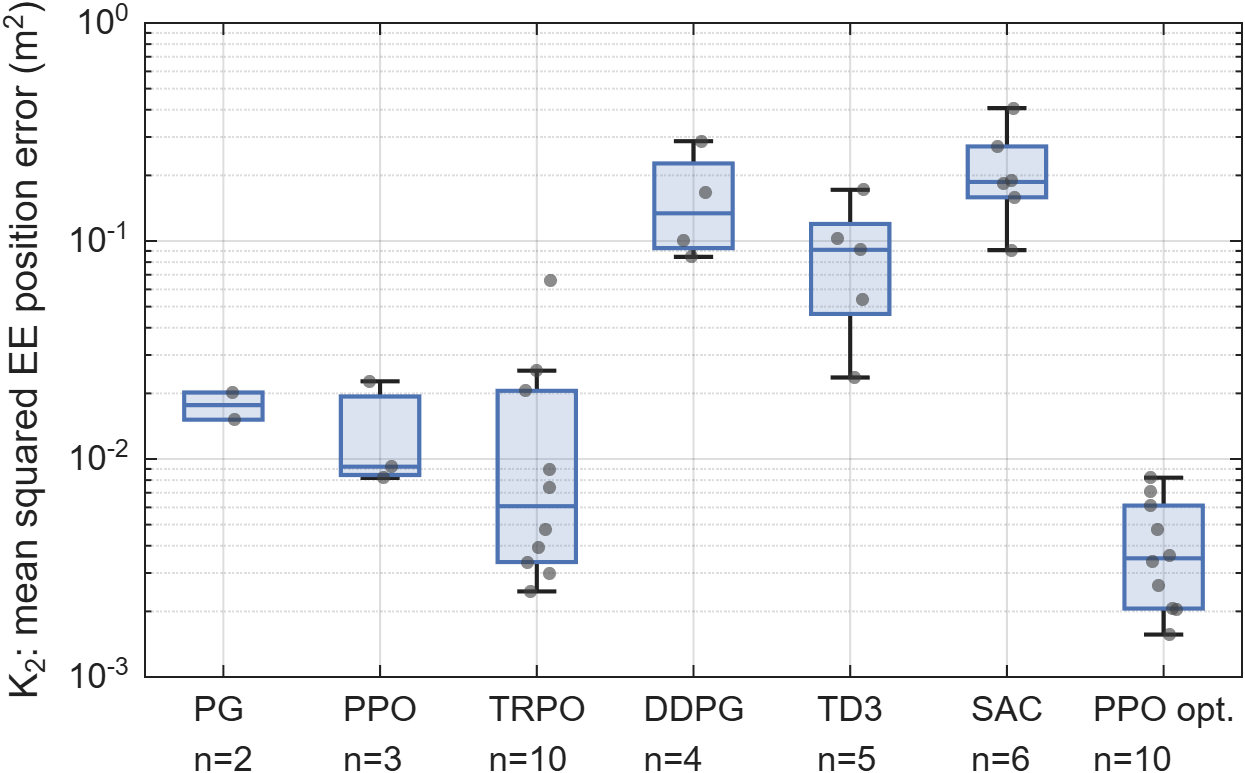
\includegraphics[width=\linewidth]{Figures/boxplot_K2.png}
    \caption{\DIFaddFL{K2: Mean Squared EE Position Error}}
    \label{fig:boxplot_k2}
  \end{subfigure}
  \hfill
  \begin{subfigure}{0.48\textwidth}
    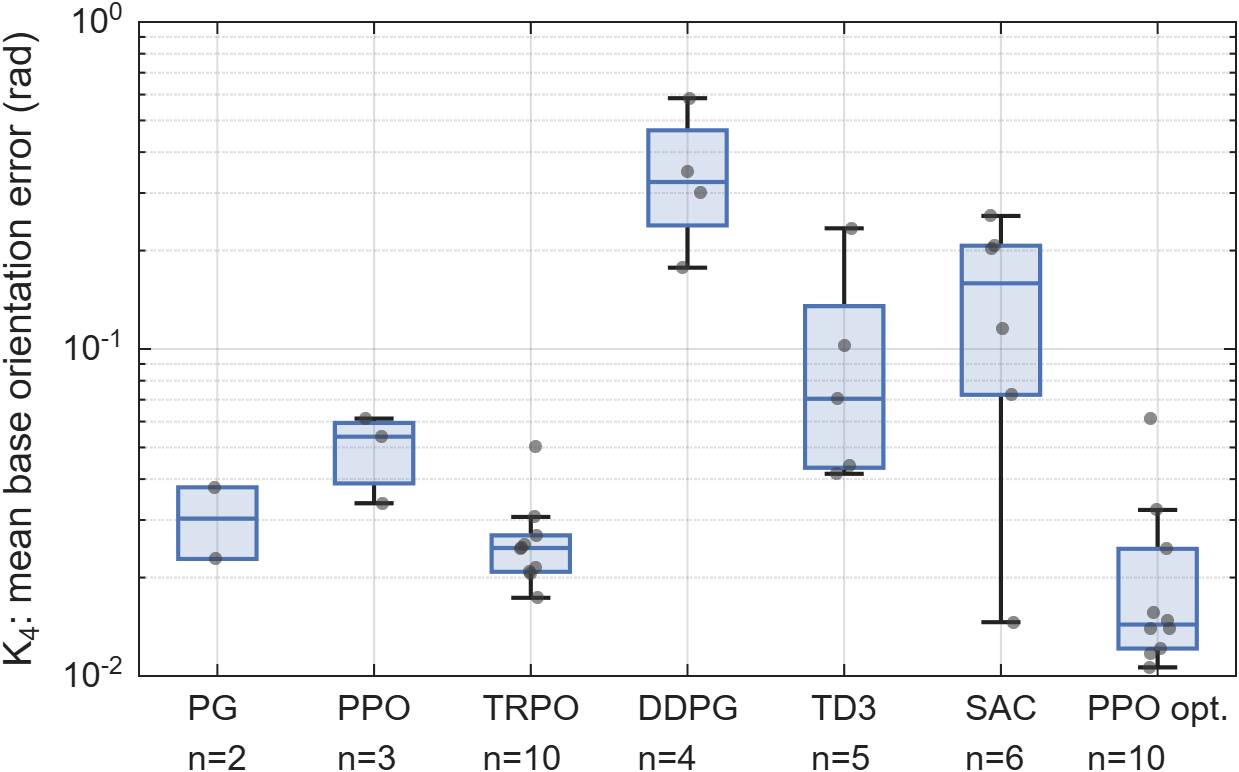
\includegraphics[width=\linewidth]{Figures/boxplot_K4.png}
    \caption{\DIFaddFL{K4: Mean Base Orientation Error}}
    \label{fig:boxplot_k4}
  \end{subfigure}
  \\[6pt]
  \begin{subfigure}{0.48\textwidth}
    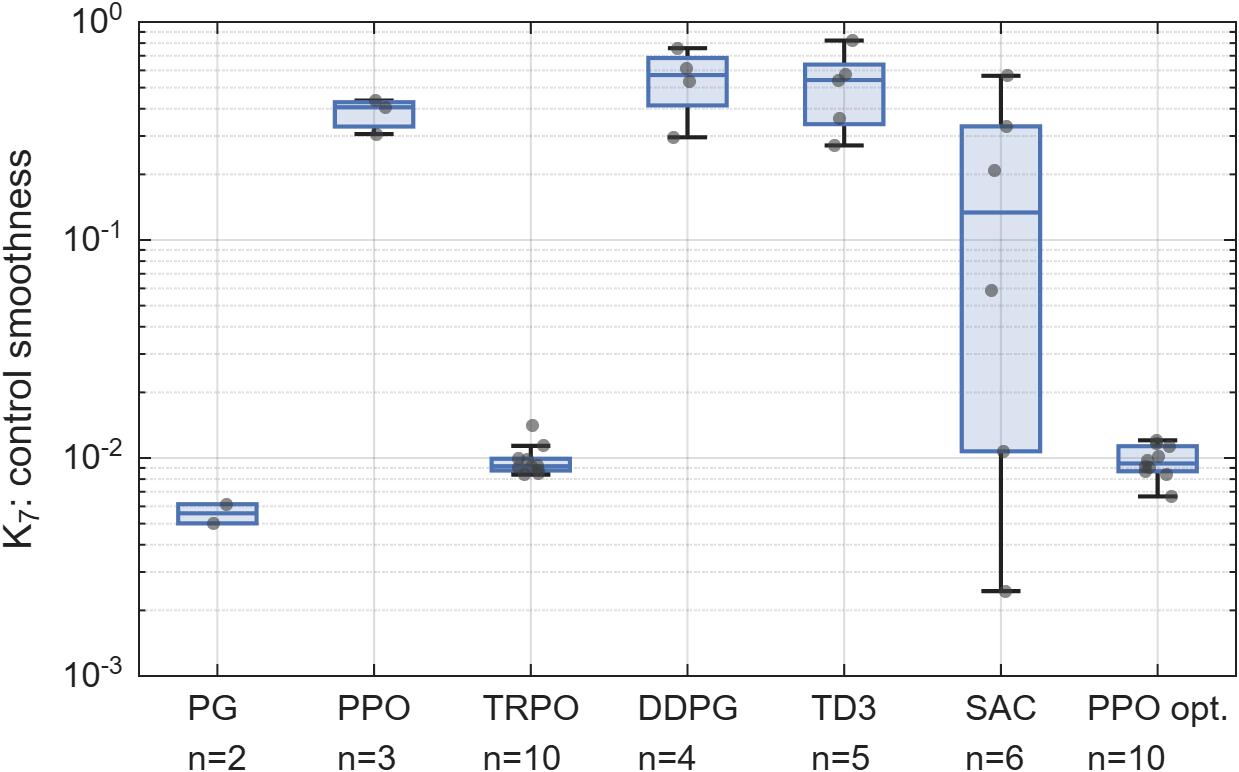
\includegraphics[width=\linewidth]{Figures/boxplot_K7.png}
    \caption{\DIFaddFL{K7: Control Smoothness (Norm.\ Jerk)}}
    \label{fig:boxplot_k7}
  \end{subfigure}
  \hfill
  \begin{subfigure}{0.48\textwidth}
    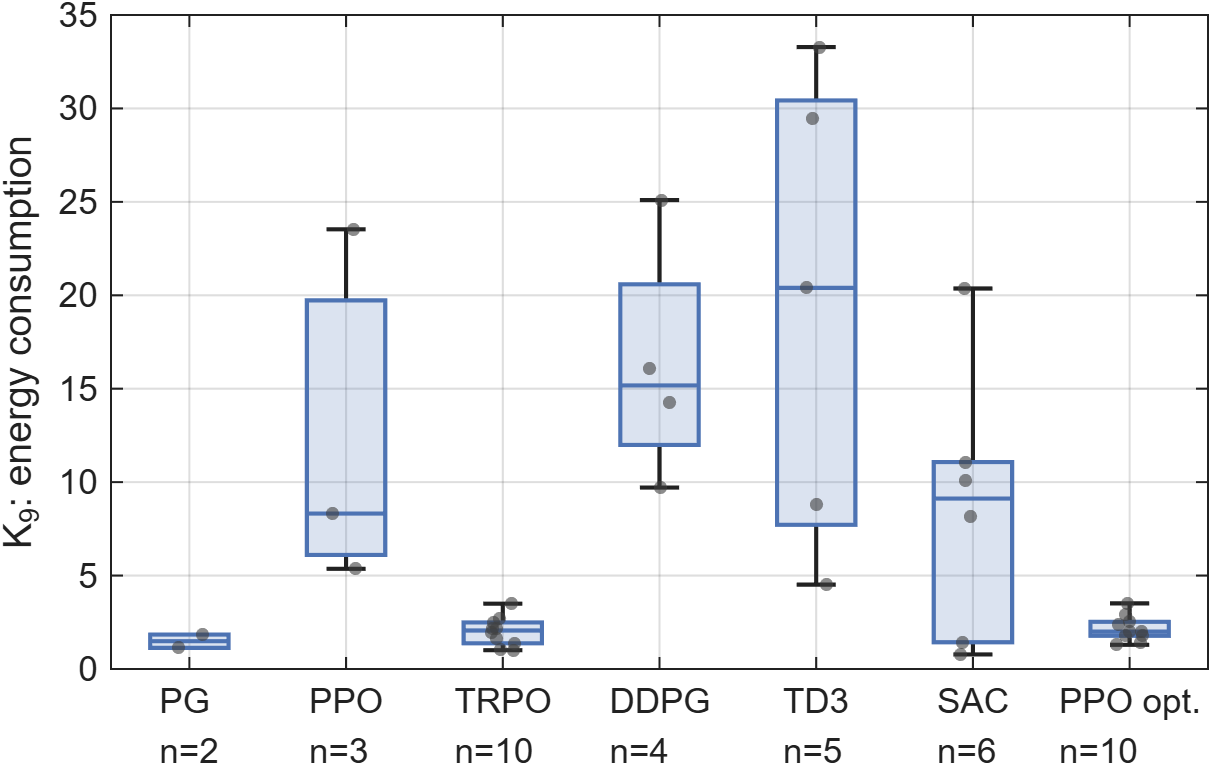
\includegraphics[width=\linewidth]{Figures/boxplot_K9.png}
    \caption{\DIFaddFL{K9: Energy Consumption}}
    \label{fig:boxplot_k9}
  \end{subfigure}
  \caption{\DIFaddFL{Boxplots of selected KPI distributions over 30 evaluation episodes per agent.
    Each box spans the interquartile range (IQR), the center line marks the median,
    the whiskers extend to 1.5\,$\times$\,IQR, and circles denote outliers.
    PPO consistently achieves low tracking error ($K_2$) and smooth control ($K_7$) with small spread,
    while PG and SAC show high variability. The low $K_9$ values for TD3 and DDPG reflect
    insufficient actuation rather than energy efficiency.}}
  \label{fig:boxplots}
\end{figure*}

\begin{figure*}[!t]
  \centering
  \begin{subfigure}{0.48\textwidth}
    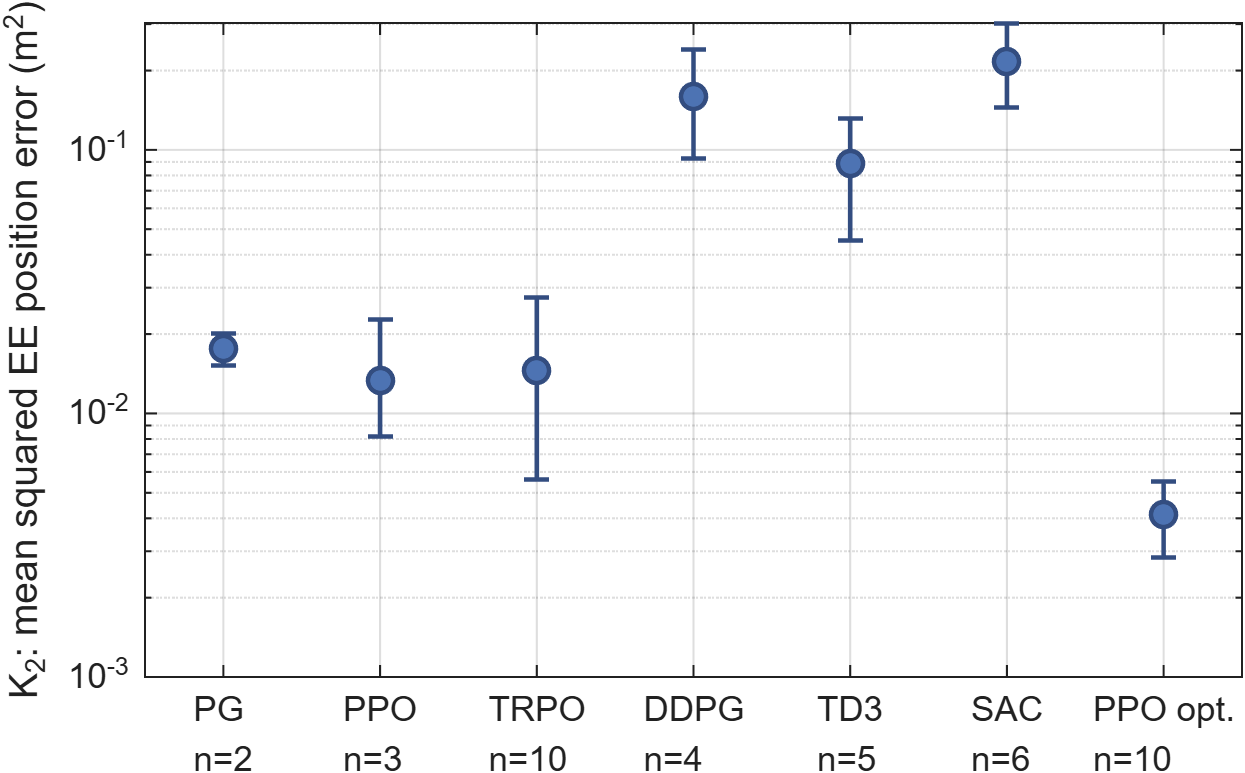
\includegraphics[width=\linewidth]{Figures/ci_K2.png}
    \caption{\DIFaddFL{K2: Mean Squared EE Position Error}}
    \label{fig:ci_k2}
  \end{subfigure}
  \hfill
  \begin{subfigure}{0.48\textwidth}
    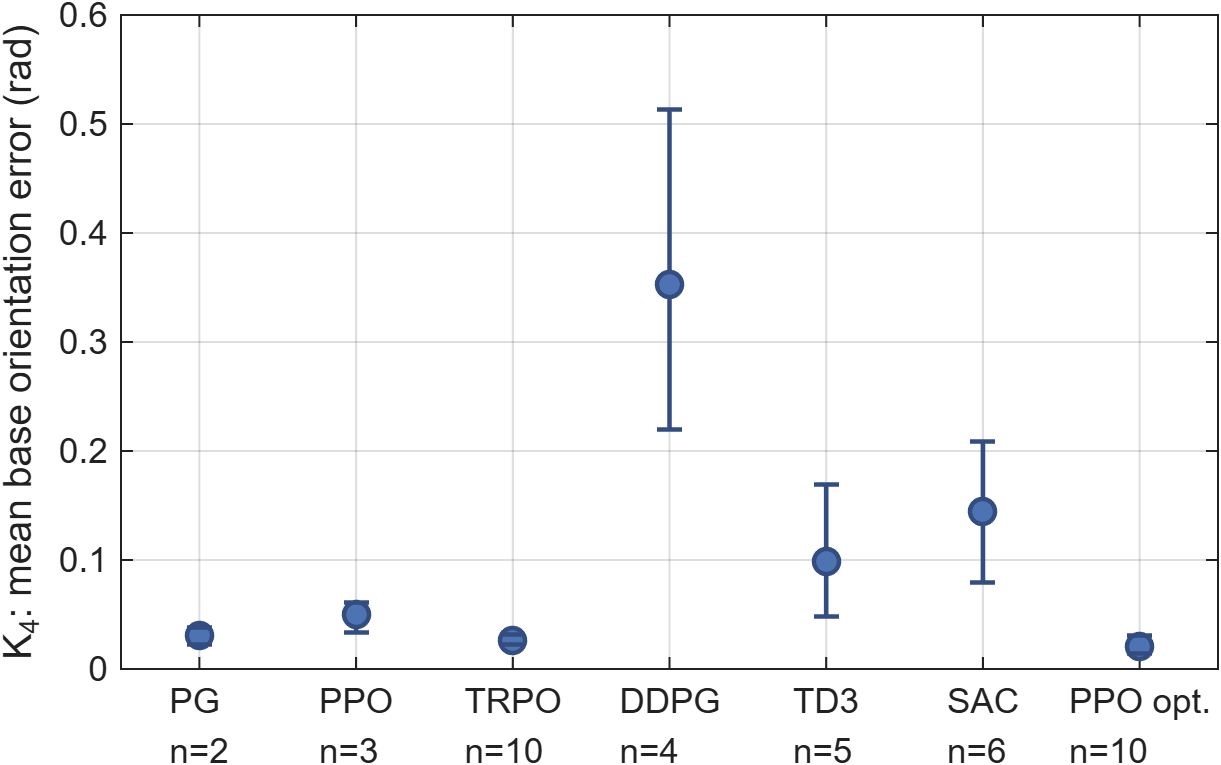
\includegraphics[width=\linewidth]{Figures/ci_K4.png}
    \caption{\DIFaddFL{K4: Mean Base Orientation Error}}
    \label{fig:ci_k4}
  \end{subfigure}
  \\[6pt]
  \begin{subfigure}{0.48\textwidth}
    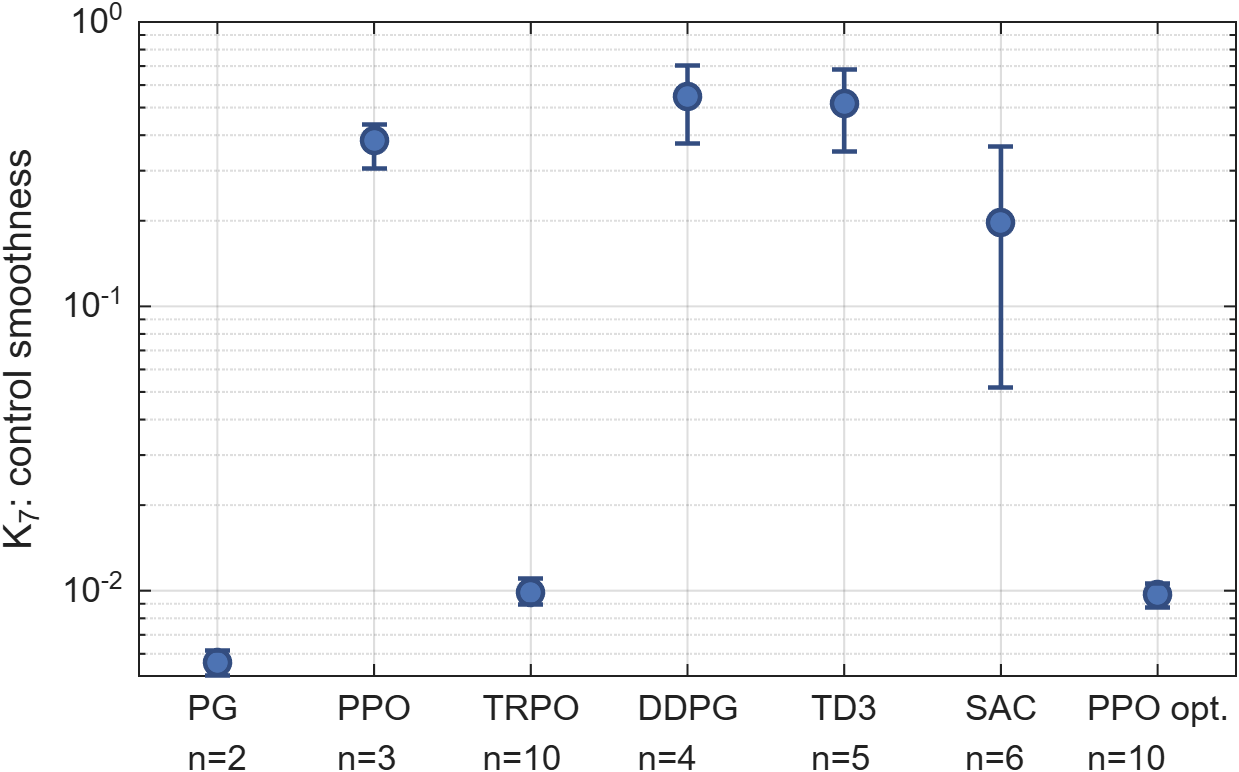
\includegraphics[width=\linewidth]{Figures/ci_K7.png}
    \caption{\DIFaddFL{K7: Control Smoothness (Norm.\ Jerk)}}
    \label{fig:ci_k7}
  \end{subfigure}
  \hfill
  \begin{subfigure}{0.48\textwidth}
    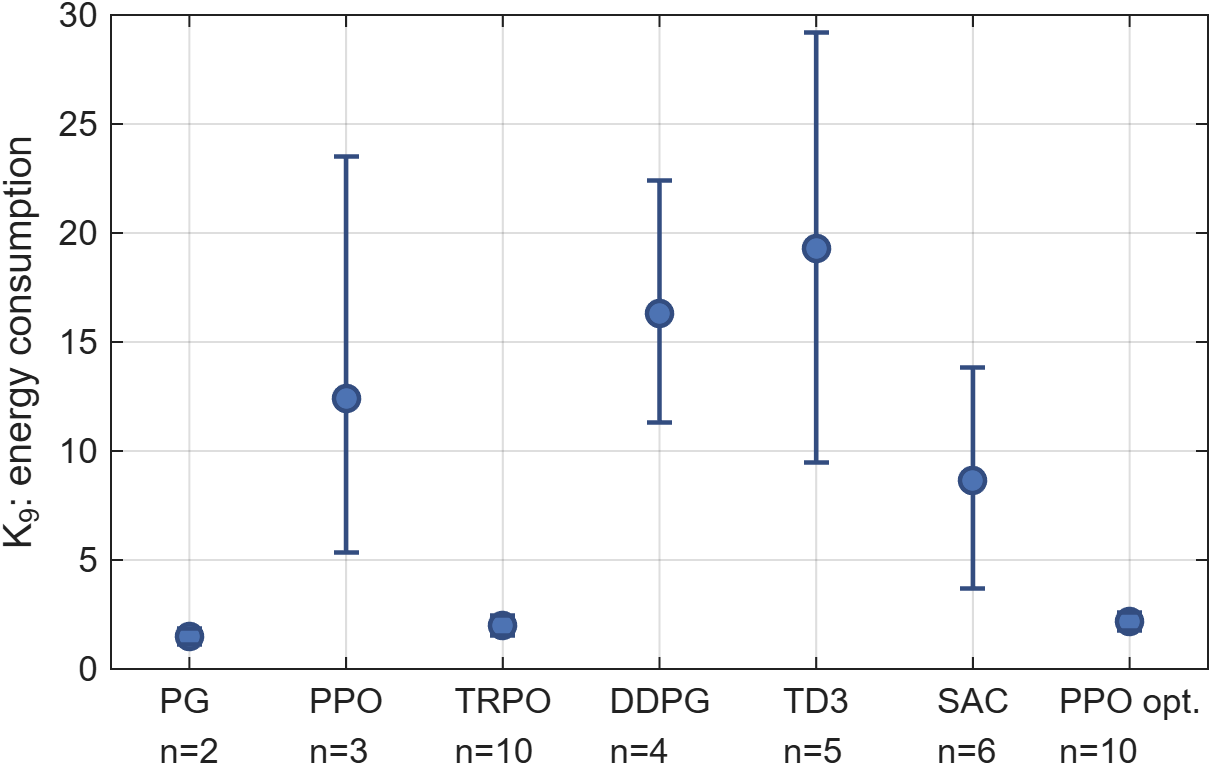
\includegraphics[width=\linewidth]{Figures/ci_K9.png}
    \caption{\DIFaddFL{K9: Energy Consumption}}
    \label{fig:ci_k9}
  \end{subfigure}
  \caption{\DIFaddFL{95\% bootstrap confidence intervals for selected KPIs across all agents
    (30 evaluation episodes per agent).
    Narrow intervals for TD3 and DDPG reflect near-constant behavior (policy collapse),
    whereas PPO's intervals are tight despite exploring the full workspace.
    TRPO and PPO show overlapping intervals for $K_4$ (base orientation), consistent with
    the non-significant Wilcoxon result ($p=0.926$).}}
  \label{fig:ci_plots}
\end{figure*}

\DIFaddend \section{Optimization of the PPO Agent}
\DIFdelbegin \DIFdel{Having identified PPO as the most promising algorithm, we focused on enhancing its performance on path tracking task of the space robot.
}\DIFdelend \DIFaddbegin \DIFadd{Based on the comparison in Section~\ref{comparison}, PPO is selected for further tuning. }\DIFaddend The PPO agent \DIFdelbegin \DIFdel{we compared above was a “default ” PPO configuration (as
}\DIFdelend \DIFaddbegin \DIFadd{used so far corresponds to the default configuration }\DIFaddend provided by MATLAB\DIFdelbegin \DIFdel{’s RL Toolbox example ) with minimal tuning \mbox{%DIFAUXCMD
\cite{b4}}\hskip0pt%DIFAUXCMD
. While it already outperformed other
agents, we hypothesized there was room to improve in terms of }\DIFdelend \DIFaddbegin \DIFadd{'s Reinforcement Learning Toolbox example \mbox{%DIFAUXCMD
\cite{b4}}\hskip0pt%DIFAUXCMD
, with minimal manual adjustment. The following modifications target three objectives: }\DIFaddend faster convergence, \DIFdelbegin \DIFdel{higher precision, and eliminating the remaining constraint violations. We therefore undertook a systematic
optimization of PPO, involving }\DIFdelend \DIFaddbegin \DIFadd{lower tracking and base-orientation errors, and avoidance of the remaining joint-limit violations. The tuning involves }\DIFaddend both network architecture \DIFdelbegin \DIFdel{modifications and hyperparameter tuning}\DIFdelend \DIFaddbegin \DIFadd{and hyperparameters}\DIFaddend .



\begin{figure*}[!t]
	\centering
	\begin{subfigure}{0.48\textwidth}
		\DIFdelbeginFL %DIFDELCMD < 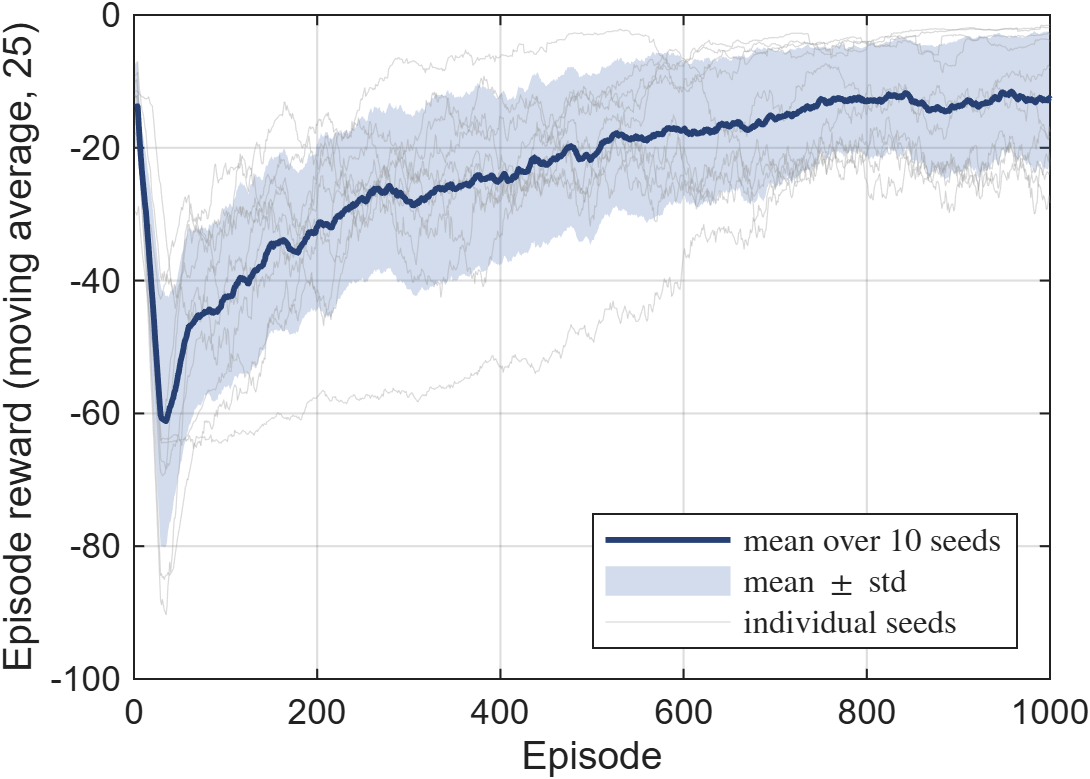
\includegraphics[width=\linewidth]{Figures/trainingsverlauf_ppo_default.png}
%DIFDELCMD < 		%%%
\DIFdelendFL \DIFaddbeginFL 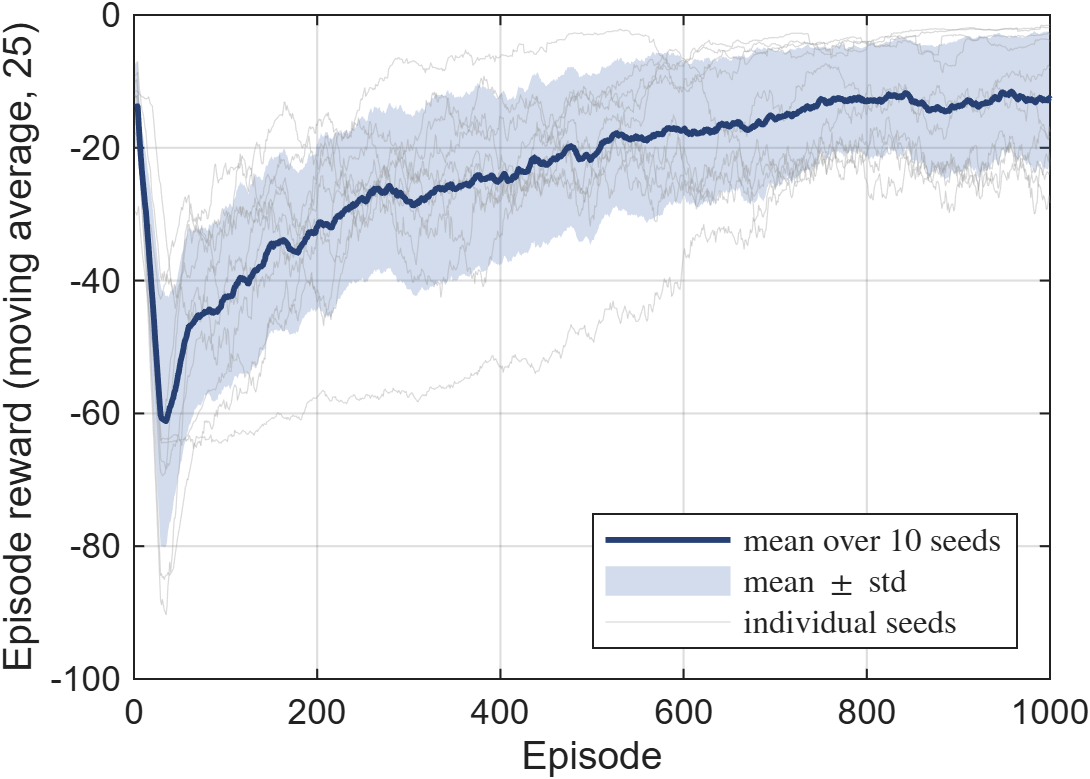
\includegraphics[width=\linewidth,height=0.25\textheight]{Figures/trainingsverlauf_ppo_default.png}
		\DIFaddendFL \caption{PPO (Default)}
		\label{fig:training_ppo_default}
	\end{subfigure}
	\hfill
	\begin{subfigure}{0.48\textwidth}
		\DIFdelbeginFL %DIFDELCMD < 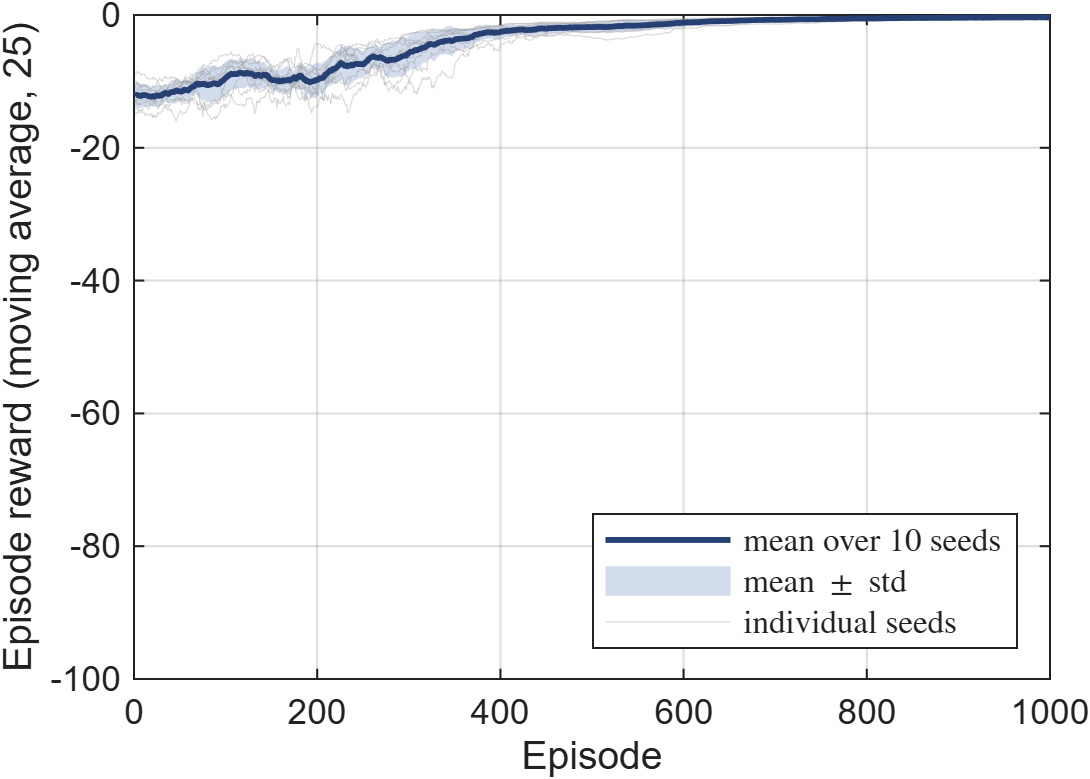
\includegraphics[width=\linewidth]{Figures/trainingsverlauf_ppo_optimized.png}
%DIFDELCMD < 		%%%
\DIFdelendFL \DIFaddbeginFL 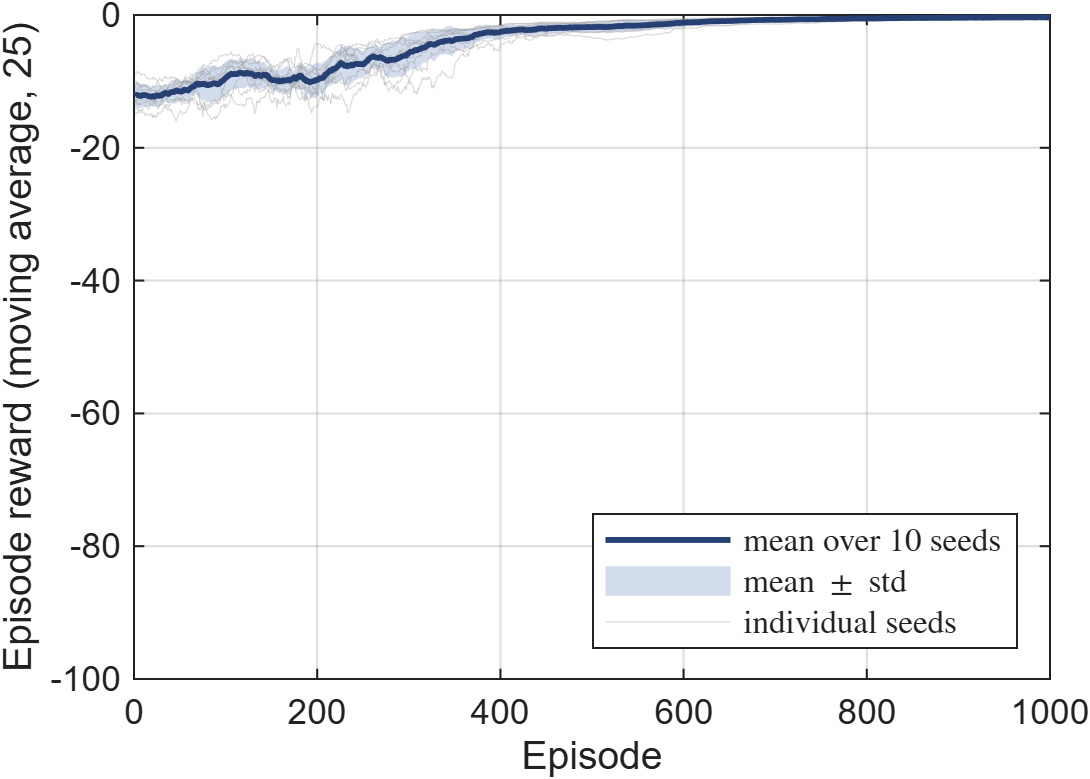
\includegraphics[width=\linewidth, height=0.25\textheight]{Figures/trainingsverlauf_ppo_optimized.png}
		\DIFaddendFL \caption{PPO (Optimized)}
		\label{fig:training_ppo_opt}
	\end{subfigure}
	\caption{Comparison of episodic rewards for default and optimized PPO agents.
  (a) Episode reward evolution during training using the default PPO hyperparameters. 
  (b) Episode reward evolution using the optimized PPO configuration.
 The optimized configuration \DIFdelbeginFL \DIFdelFL{exhibits }\DIFdelendFL \DIFaddbeginFL \DIFaddFL{shows }\DIFaddendFL faster convergence and \DIFaddbeginFL \DIFaddFL{a }\DIFaddendFL higher average \DIFdelbeginFL \DIFdelFL{episode rewards, 
 indicating improved learning efficiency and policy performance}\DIFdelendFL \DIFaddbeginFL \DIFaddFL{episodic return than the
 default configuration}\DIFaddendFL .}
	\label{fig:training_ppo_compare}
\end{figure*}
\noindent

\DIFdelbegin \DIFdel{Network Architecture Improvements: By default , the PPO agent used }\DIFdelend \DIFaddbegin \textbf{\DIFadd{Network architecture.}} \DIFadd{The default PPO agent uses }\DIFaddend two hidden layers of 128
\DIFdelbegin \DIFdel{neurons each (}\DIFdelend \DIFaddbegin \DIFadd{units each }\DIFaddend with ReLU activations \DIFdelbegin \DIFdel{) }\DIFdelend for both the policy and \DIFdelbegin \DIFdel{value function networks. We
experimented }\DIFdelend \DIFaddbegin \DIFadd{the value network. Variants }\DIFaddend with deeper and wider networks \DIFdelbegin \DIFdel{, as well as }\DIFdelend \DIFaddbegin \DIFadd{and with }\DIFaddend alternative activation functions \DIFdelbegin \DIFdel{, to better
capture the dynamics of the problem. Our optimized architecture ultimately used 3 hidden layers }\DIFdelend \DIFaddbegin \DIFadd{were evaluated. The selected architecture uses three hidden layers of sizes $[256, 256, 128]$ }\DIFaddend for the policy network \DIFdelbegin \DIFdel{with layer sizes }%DIFDELCMD < [%%%
\DIFdel{256, 256, 128}%DIFDELCMD < ] %%%
\DIFdel{and 2 hidden layers }\DIFdelend \DIFaddbegin \DIFadd{and two hidden layers of sizes $[256, 128]$ }\DIFaddend for the value network\DIFdelbegin \DIFdel{with sizes
}%DIFDELCMD < [%%%
\DIFdel{256, 128}%DIFDELCMD < ]%%%
\DIFdel{. We found that the }\DIFdelend \DIFaddbegin \DIFadd{. The }\DIFaddend additional depth and capacity \DIFdelbegin \DIFdel{in }\DIFdelend \DIFaddbegin \DIFadd{of }\DIFaddend the policy network \DIFdelbegin \DIFdel{helped the agent learn
the intricate relationship between arm motions and base reactions (especially given }\DIFdelend \DIFaddbegin \DIFadd{reduce the tracking error and }\DIFaddend the \DIFaddbegin \DIFadd{base-orientation error (cf.\ }\autoref{tab:ppo_optimization_kpi}\DIFadd{) for the }\DIFaddend 23-dimensional state input \DIFdelbegin \DIFdel{) \mbox{%DIFAUXCMD
\cite{b4}}\hskip0pt%DIFAUXCMD
. We also introduced layer normalization in }\DIFdelend \DIFaddbegin \DIFadd{\mbox{%DIFAUXCMD
\cite{b4}}\hskip0pt%DIFAUXCMD
. Layer normalization is applied to }\DIFaddend the first layer to \DIFdelbegin \DIFdel{help stabilize learning,
given }\DIFdelend \DIFaddbegin \DIFadd{compensate for }\DIFaddend the different scales of \DIFaddbegin \DIFadd{the }\DIFaddend input features (\DIFdelbegin \DIFdel{joint angles vs. orientation quaternions, etc.}\DIFdelend \DIFaddbegin \DIFadd{e.g., joint angles versus orientation quaternions}\DIFaddend ). The activation function \DIFdelbegin \DIFdel{remained ReLU, which was sufficient. These architecture changes were implemented by
explicitly defining the neural network layers instead of using the auto-generated default network.
In summary, the optimized policy network was larger and potentially more expressive, which we believe
allowed PPO to find a control strategy which is better tuned. }\DIFdelend \DIFaddbegin \DIFadd{is kept as ReLU. The networks are defined explicitly rather than through the toolbox default constructor.
}\DIFaddend 

\DIFdelbegin \DIFdel{Hyperparameter Tuning: We systematically varied key PPO hyperparameters and evaluated their impact on training curves (learning speed and stability):
}\DIFdelend \DIFaddbegin \textbf{\DIFadd{Hyperparameter Tuning.}} \DIFadd{The optimization followed a coordinate-wise grid search. Each hyperparameter was swept across a discrete set of candidate values while all others were held at their current best, and the configuration yielding the highest mean episodic reward over the final 50 training episodes (out of $N_{\text{train}}=1000$) was selected. In total, 16 training runs of 1000 episodes each were conducted during this tuning phase. The swept parameters, their candidate values, and the selected values are as follows:
}\DIFaddend \begin{itemize}
  \item \DIFdelbegin \DIFdel{The learning rate was tuned: the default was 1e-3. We found that a slightly lower learning rate
(e.g. 5e-4) improved stability (preventing overshooting in policy updates) without  slowing
convergence.
  }\DIFdelend \DIFaddbegin \textbf{\DIFadd{Actor learning rate.}} \DIFadd{Candidates $\{1\!\times\!10^{-3},\;5\!\times\!10^{-4}\}$, selected $5\!\times\!10^{-4}$. The lower rate reduced overshooting in policy gradient updates, improving convergence stability.
  }\DIFaddend \item \DIFdelbegin \DIFdel{The mini-batch size for stochastic gradient descent updates was increased. By default, PPO
might use a batch of 64 from each trajectory. We increased this to 256 to provide more stable
gradient estimates per update, which helped reduce the variance in training. }%DIFDELCMD < \item %%%
\item%DIFAUXCMD
\DIFdel{The clip ratio ($\epsilon$) for PPO’s surrogate objective was adjusted. The default clip value 0.2 worked, but we tried slightly tighter (0.15) and looser (0.3) clips \mbox{%DIFAUXCMD
\cite{b15}}\hskip0pt%DIFAUXCMD
. A tighter clip ($\epsilon$ = 0.1–0.15) made updates
more conservative. This reduced occasional policy overshoots at the cost of slower improvement.
We settled on $\epsilon\approx0.2$ as it was already near-optimal, but this process confirmed that too high a
clip would harm stability. The clip factor $\epsilon$ in PPO limits the magnitude of policy updates by constraining 
the probability ratio between the new and the old policy . This prevents excessively large policy updates that could 
destabilize training, particularly in highly nonlinear control tasks.
  In safety-critical scenarios such as free-floating 
space robot control, clipping contributes significantly to stable and reliable convergence \mbox{%DIFAUXCMD
\cite{b4,b15}}\hskip0pt%DIFAUXCMD
. }\DIFdelend \DIFaddbegin \textbf{\DIFadd{Critic learning rate.}} \DIFadd{Candidates $\{1\!\times\!10^{-3},\;5\!\times\!10^{-4}\}$, selected $1\!\times\!10^{-3}$. A higher critic learning rate allowed the value function to track the evolving policy more closely, providing more accurate advantage estimates.
  }\DIFaddend \item \DIFdelbegin \DIFdel{Entropy regularization weight was tuned. PPO can include an entropy term to encourage
exploration. We increased the entropy coefficient modestly (from 0 to 0.01) to avoid }\DIFdelend \DIFaddbegin \textbf{\DIFadd{Entropy loss weight.}} \DIFadd{Candidates $\{1\!\times\!10^{-2},\;1\!\times\!10^{-3}\}$, selected $1\!\times\!10^{-3}$. A small entropy bonus discouraged }\DIFaddend premature convergence to a suboptimal deterministic policy \DIFdelbegin \DIFdel{. This indeed improved the exploration in early
training, helping the agent discover better strategies (like moving joints in opposite directions to
}\DIFdelend \DIFaddbegin \DIFadd{and encouraged the agent to discover strategies such as coordinated joint motions that }\DIFaddend cancel base momentum\DIFdelbegin \DIFdel{)}\DIFdelend \DIFaddbegin \DIFadd{, without causing aimless exploration}\DIFaddend .
  \item \DIFdelbegin \DIFdel{Discount factor ($\gamma$) and GAE (Generalized Advantage Estimation) parameter ($\lambda$) were left at
standard values ($\gamma = 0.99$, $\lambda = 0.95$) after confirming that they already provided a good bias-variance trade-off for advantage estimation
  }\DIFdelend \DIFaddbegin \textbf{\DIFadd{Experience horizon.}} \DIFadd{Candidates $\{512,\;1024,\;2048\}$, selected $1024$. A moderate rollout horizon provided sufficient trajectory information per update while keeping memory requirements and update latency manageable.
  }\DIFaddend \item \DIFdelbegin \DIFdel{We also adjusted the target KL-divergence for PPO’s stopping criteria (if used) to ensure the
policy updates didn’t diverge. We monitored the KL and it remained within acceptable
}%DIFDELCMD < {%%%
\DIFdel{range with our chosen settings.
}%DIFDELCMD < }
%DIFDELCMD < %%%
\DIFdelend \DIFaddbegin \textbf{\DIFadd{Mini-batch size.}} \DIFadd{Candidates $\{128,\;256\}$, selected $256$. Larger batches provided more stable gradient estimates per update, reducing training variance.
}\DIFaddend \end{itemize}

\DIFdelbegin \DIFdel{Through a grid search over these parameters (one at a time and some combined), we converged on a
set }\DIFdelend \DIFaddbegin \DIFadd{This process yielded a configuration }\DIFaddend that provided a more stable and higher-performing PPO agent. Notably, the \DIFdelbegin \DIFdel{optimized agent
is tailored to this specific task and reward function, for example, the entropy bonus was chosen to the
point where it encourages exploration of different arm motions, but not so high that the agent keeps thrashing
the arm aimlessly}\DIFdelend \DIFaddbegin \DIFadd{asymmetric learning rates, a slower actor ($5\!\times\!10^{-4}$) paired with a faster critic ($1\!\times\!10^{-3}$), reflect the different roles of the two networks. The value function must adapt quickly to policy changes, while conservative actor updates prevent destabilizing the learned control strategy}\DIFaddend .

\subsection{Circular Trajectory}

\DIFdelbegin \DIFdel{Training Outcome: The effects of these optimizations were evident }\DIFdelend \DIFaddbegin \textbf{\DIFadd{Training outcome.}} \DIFadd{The effect of the modifications can be seen }\DIFaddend in the training \DIFdelbegin \DIFdel{learning }\DIFdelend curves (see~\autoref{fig:training_ppo_compare}). The default PPO agent\DIFdelbegin \DIFdel{’s learning curve initially rose, but then plateaued at a fairly
negative reward value (\textasciitilde-2 per episode ) and exhibited high variance even after many episodes. This
plateau suggested it reached }\DIFdelend \DIFaddbegin \DIFadd{'s episodic return increases initially and then plateaus around $-2$ per episode with high variance over the remaining training, indicating convergence to }\DIFaddend a suboptimal policy\DIFdelbegin \DIFdel{and struggled to improve further}\DIFdelend . In contrast, the optimized PPO agent\DIFdelbegin \DIFdel{’s learning curve kept rising steadily and converged to a much higher average
reward (less negative, }\DIFdelend \DIFaddbegin \DIFadd{'s return continues to increase and converges to a higher value (}\DIFaddend closer to zero) with \DIFdelbegin \DIFdel{significantly }\DIFdelend reduced variance. Table~\ref{tab:ppo_optimization_kpi} reports the KPI averages over \DIFdelbegin \DIFdel{$N_{eval}=30$ }\DIFdelend \DIFaddbegin \DIFadd{$N_{\mathrm{eval}} = 30$ }\DIFaddend evaluation episodes for PPO with the default \DIFdelbegin \DIFdel{configuration }\DIFdelend and the optimized \DIFdelbegin \DIFdel{configuration. Specifically, where the
default PPO leveled off around -2.0 cumulative reward, the optimized PPO approached -0.4 on average,
a dramatic improvement. The variability (shaded region in the reward plot) shrank, indicating the
agent’s behavior became consistently optimal across training episodes. Quantitatively, the
mean episodic reward K1 improved from -2.23 (default PPO ) to -0.43 (optimized PPO). This
roughly fivefold increase in reward corresponds to the agent accomplishing much more of the task
(since zero would be perfect tracking with no penalties). The lower variance also hints that the agent not
only improved its average performance but did so reliably without frequent failures}\DIFdelend \DIFaddbegin \DIFadd{configurations. The mean episodic return $K_1$ increases from $-2.23$ for the default PPO to $-0.43$ for the optimized PPO, an increase by a factor of approximately five. The reduced variance indicates that the improvement is consistent across episodes rather than driven by a few outliers}\DIFaddend .

\begin{figure*}[!t]
    \centering
    \begin{subfigure}{0.48\textwidth}
        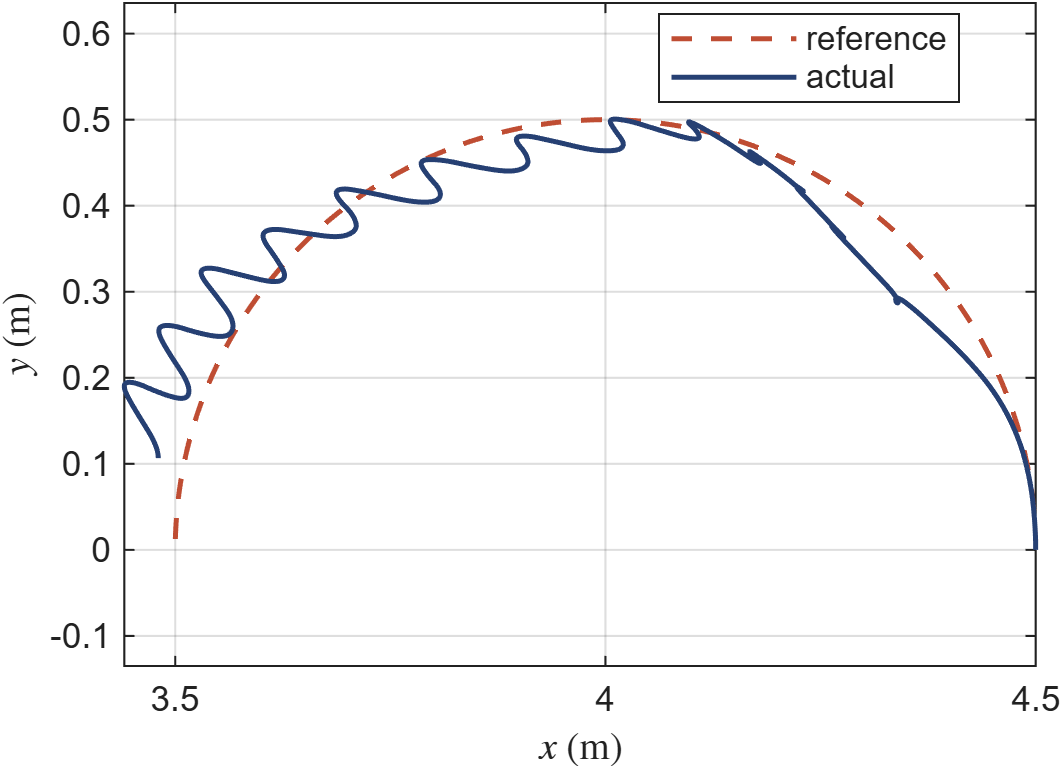
\includegraphics[width=\linewidth]{Figures/soll_vs_ist_kreisbahn.png}
        \caption{PPO (Default)}
        \label{fig:traj_default}
    \end{subfigure}
    \hfill
    \begin{subfigure}{0.48\textwidth}
        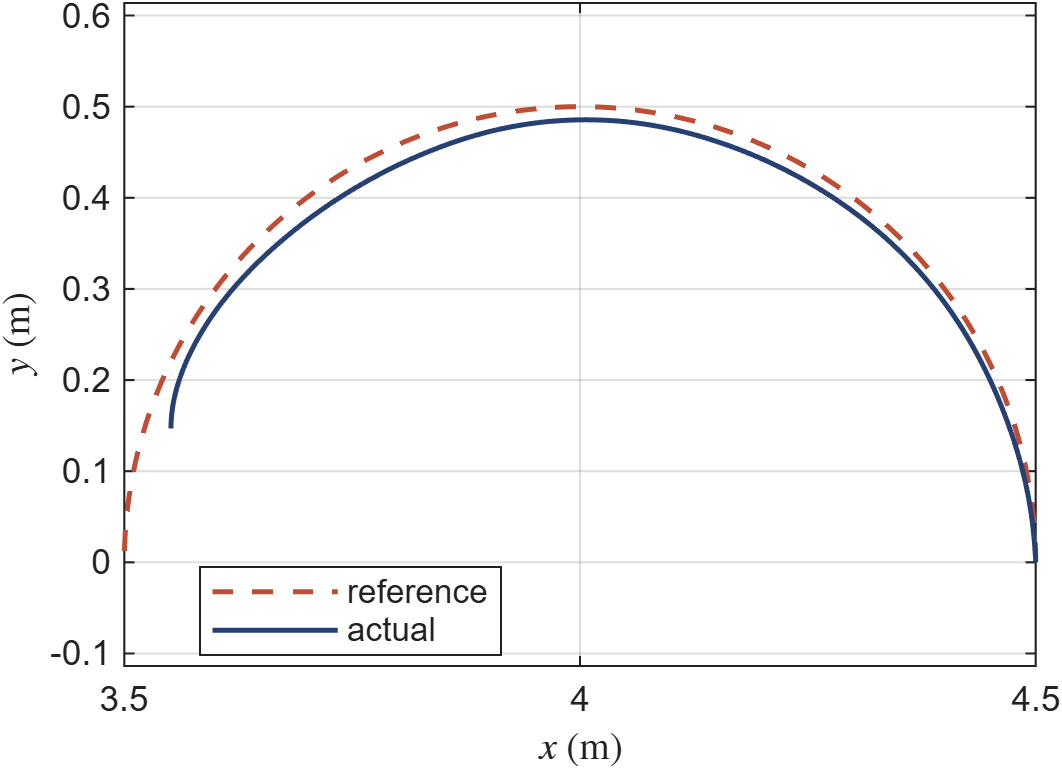
\includegraphics[width=\linewidth]{Figures/soll_vs_ist_kreisbahn_opt.png}
        \caption{PPO (Optimized)}
        \label{fig:traj_opt}
    \end{subfigure}
    \caption{Target/actual comparison of the end-effector trajectory in the XY plane.}
    \label{fig:trajektorie_xy_compare}
\end{figure*}

\begin{figure*}[!t]
    \centering
    \begin{subfigure}{0.48\textwidth}
        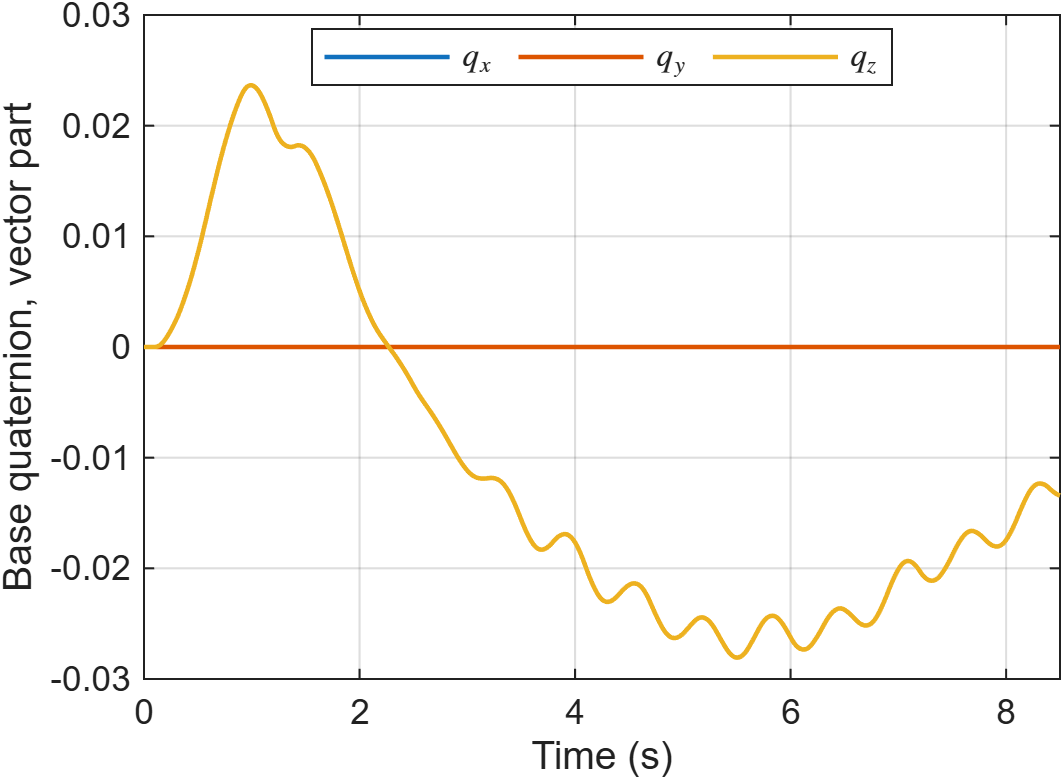
\includegraphics[width=\linewidth]{Figures/basis_orientaion_ppo.png}
        \caption{PPO (Default)}
        \label{fig:basis_default}
    \end{subfigure}
    \hfill
    \begin{subfigure}{0.48\textwidth}
        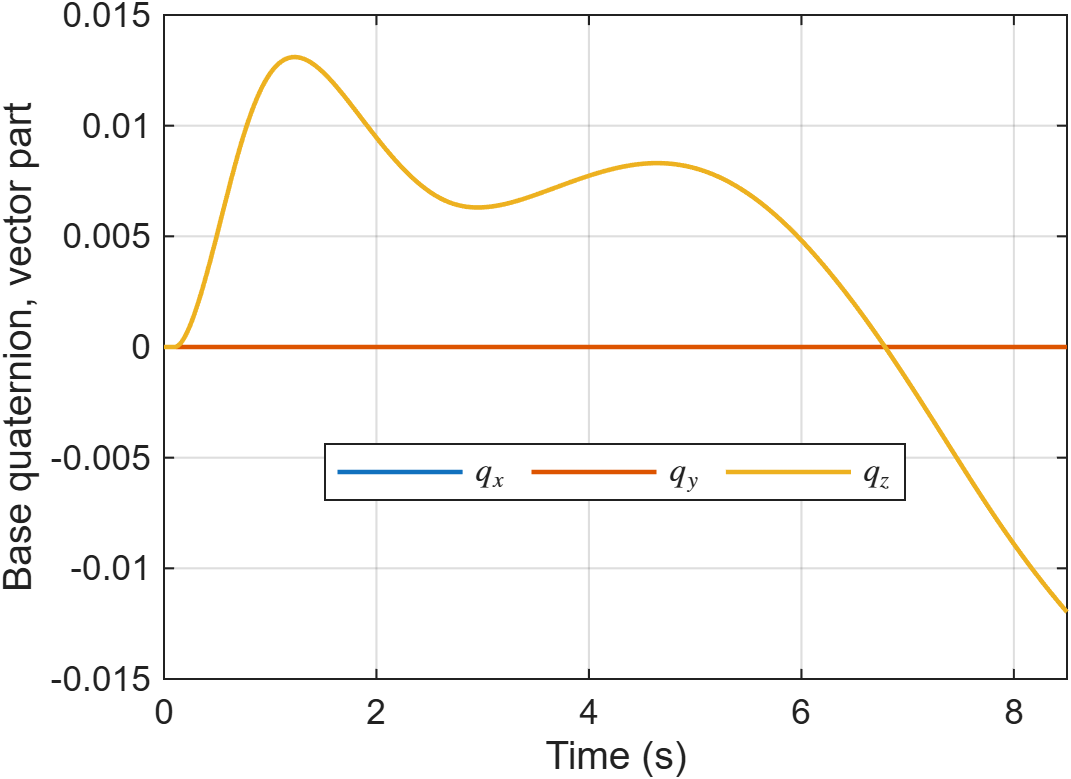
\includegraphics[width=\linewidth]{Figures/basis_orientation_ppo_optimized.png}
        \caption{PPO (Optimized)}
        \label{fig:basis_opt}
    \end{subfigure}
    \caption{\DIFdelbeginFL \DIFdelFL{Course }\DIFdelendFL \DIFaddbeginFL \DIFaddFL{Time evolution }\DIFaddendFL of \DIFaddbeginFL \DIFaddFL{the }\DIFaddendFL base orientation (quaternion components) during a test episode.}
    \label{fig:basis_orientation_compare}
\end{figure*}

\begin{table}[!b]
	\centering
	\caption{Performance of PPO agent before and after optimization. The optimized PPO \DIFdelbeginFL \DIFdelFL{shows substantial
		improvements in all aspects (}\DIFdelendFL \DIFaddbeginFL \DIFaddFL{improves most reported
		KPIs, with }\DIFaddendFL higher rewards, lower errors, \DIFdelbeginFL \DIFdelFL{zero }\DIFdelendFL \DIFaddbeginFL \DIFaddFL{no observed }\DIFaddendFL safety violations \DIFaddbeginFL \DIFaddFL{in the evaluation episodes}\DIFaddendFL , \DIFdelbeginFL \DIFdelFL{smoother }\DIFdelendFL and \DIFdelbeginFL \DIFdelFL{more
		efficient }\DIFdelendFL \DIFaddbeginFL \DIFaddFL{smoother
		}\DIFaddendFL control\DIFdelbeginFL \DIFdelFL{)}\DIFdelendFL .}
    \label{tab:ppo_optimization_kpi}
	\renewcommand{\arraystretch}{1.2}
	\setlength{\tabcolsep}{3pt}
	\DIFdelbeginFL %DIFDELCMD < \begin{tabular}{lcc}
%DIFDELCMD < 		\toprule
%DIFDELCMD < 		\textbf{Metric (KPI)} & \textbf{PPO (Default)} & \textbf{PPO (Optimized)} \\
%DIFDELCMD < 		\midrule
%DIFDELCMD < 		Mean Episodic Reward (K1)        & $-2.23$  & $\mathbf{-0.43}$ \\
%DIFDELCMD < 		Mean Squared EE Tracking Error (K2)      & 0.0257  & \textbf{0.0083} \\
%DIFDELCMD < 		Max EE Tracking Error (K3)       & 0.4833   & \textbf{0.27} \\
%DIFDELCMD < 		Mean Base Orientation Error (K4) & 0.0667  & \textbf{0.022} \\
%DIFDELCMD < 		Collision Rate (K5)             & 0 & 0 \\
%DIFDELCMD < 		Joint Limit Violation Rate (K6) & 0.0505 (5.1\%) & \textbf{0} \\
%DIFDELCMD < 		Torque Smoothness (K7, jerk)     & 0.6812  & \textbf{0.351} \\
%DIFDELCMD < 		Energy Consumption (K9)          & 6.325  & \textbf{5.314} \\
%DIFDELCMD < 		\bottomrule
%DIFDELCMD < 	\end{tabular}
%DIFDELCMD < %%%
\DIFdelendFL \DIFaddbeginFL \begin{tabular}{lcc}
		\toprule
		\textbf{Metric (KPI)} & \textbf{PPO (Default)} & \textbf{PPO (Optimized)} \\
		\midrule
		Mean Episodic Reward (K1)        & $-2.23$  & $\mathbf{-0.43}$ \\
		Mean Squared EE Tracking Error (K2)      & 0.0257  & \textbf{0.0083} \\
		Max EE Tracking Error (K3)       & 0.4833   & \textbf{0.27} \\
		Mean Base Orientation Error (K4) & 0.0667  & \textbf{0.022} \\
		Collision Rate (K5)             & 0 & 0 \\
		Joint Limit Violation Rate (K6) & 0.0505 (5.1\%) & \textbf{0} \\
		Torque Smoothness (K7, jerk)     & 0.6812  & \textbf{0.351} \\
		Mean Base Angular Velocity (K8)  & 0.095  & \textbf{0.050} \\
		Energy Consumption (K9)          & 6.325  & \textbf{5.314} \\
		\bottomrule
	\end{tabular}
\DIFaddendFL \end{table}

\DIFdelbegin \DIFdel{Beyond the reward improvement , the optimizations translate directly to task }\DIFdelend \DIFaddbegin \DIFadd{The reward improvement translates directly into task-level }\DIFaddend performance. \autoref{fig:trajektorie_xy_compare}
shows the end-effector path in the \DIFdelbegin \DIFdel{XY-plane}\DIFdelend \DIFaddbegin \DIFadd{$XY$ plane}\DIFaddend : the default PPO deviates \DIFdelbegin \DIFdel{significantly }\DIFdelend from the reference circle and exhibits \DIFdelbegin \DIFdel{jagged oscillations, whereas }\DIFdelend \DIFaddbegin \DIFadd{oscillations, while }\DIFaddend the optimized PPO \DIFdelbegin \DIFdel{traces the referencealmost exactly}\DIFdelend \DIFaddbegin \DIFadd{closely follows the reference}\DIFaddend . The mean squared tracking error \DIFdelbegin \DIFdel{K2 dropped from 0.0257 to 0.0083 (a 67.7\% reduction }\DIFdelend \DIFaddbegin \DIFadd{$K_2$ decreases from $0.0257$ to $0.0083$ (a reduction of $67.7\%$}\DIFaddend ), and the maximum error \DIFdelbegin \DIFdel{K3 decreased from 0.4833 to 0.27}\DIFdelend \DIFaddbegin \DIFadd{$K_3$ from $0.4833$ to $0.27$}\DIFaddend .

Base stabilization \DIFdelbegin \DIFdel{improved markedly }\DIFdelend \DIFaddbegin \DIFadd{improves accordingly }\DIFaddend (\autoref{fig:basis_orientation_compare}): the mean orientation error \DIFdelbegin \DIFdel{K4 fell from 0.0667 to 0.022 (factor $\approx$\,3}\DIFdelend \DIFaddbegin \DIFadd{$K_4$ decreases from $0.0667$ to $0.022$ (a factor of approximately three}\DIFaddend ), and the mean angular velocity \DIFdelbegin \DIFdel{K8 was halved from 0.095 to 0.050\,rad/s}\DIFdelend \DIFaddbegin \DIFadd{$K_8$ decreases from $0.095\,\mathrm{rad/s}$ to $0.050\,\mathrm{rad/s}$}\DIFaddend . The optimized agent \DIFdelbegin \DIFdel{learned }\DIFdelend \DIFaddbegin \DIFadd{uses }\DIFaddend arm motions that \DIFdelbegin \DIFdel{effectively cancel }\DIFdelend \DIFaddbegin \DIFadd{compensate for }\DIFaddend momentum transfer to the base.

\DIFdelbegin \DIFdel{The optimized PPOalso eliminated all safety violations (K5\,=\,K6\,=\,0 over }\DIFdelend \DIFaddbegin \DIFadd{For the optimized PPO, no safety violations are observed ($K_5 = K_6 = 0$ over the }\DIFaddend 30 \DIFaddbegin \DIFadd{evaluation }\DIFaddend episodes, compared to \DIFdelbegin \DIFdel{5.1\% joint-limit violations }\DIFdelend \DIFaddbegin \DIFadd{$K_6 = 5.1\%$ }\DIFaddend for the default \DIFdelbegin \DIFdel{), 
improved }\DIFdelend \DIFaddbegin \DIFadd{configuration). It also improves }\DIFaddend torque smoothness (\DIFdelbegin \DIFdel{K7: 0.6812$\to$0.351) }\DIFdelend \DIFaddbegin \DIFadd{$K_7$}\DIFaddend , \DIFaddbegin \DIFadd{$0.6812 \to 0.351$) and reduces the energy consumption by $16\%$ ($K_9$, $6.325 \to 5.314$). These changes are observed simultaneously in the reported evaluation, without an apparent trade-off among the selected KPIs.
}

\DIFadd{The optimized PPO agent satisfies the task objectives considered here in combination in the reported evaluation, namely tracking accuracy, base disturbance, safety constraints, control smoothness, and energy consumption. These results support the use of systematic hyperparameter tuning and tailored network design for safety-critical space-robot control under the considered conditions.
}

\subsection{\DIFadd{Ablation Study of Reward Components}}\label{sec:reward_ablation}
\DIFadd{To quantify the contribution of each individual term in the composite reward function defined in~}\autoref{eq:reward}\DIFadd{,
an ablation study was performed in which the optimized PPO agent was retrained on the circular trajectory with one reward component
disabled at a time. Each of the seven weights in the cost term $c_t$ was set to zero in turn while keeping the remaining six at
their baseline values ($W_p=150$, $W_v=25$, $W_{\mathrm{ori}}=200$, $W_{wb}=8$, $W_{vb}=2$, $W_u=0.02$, $W_d=0.06$). In addition,
the two positive reward terms were separately disabled by setting $r_{\text{prog}}=0$ }\DIFaddend and \DIFdelbegin \DIFdel{reduced energy consumptionby 16\% (}\DIFdelend \DIFaddbegin \DIFadd{$r_{\text{bonus}}=0$, respectively,
to isolate the contribution of the progress signal and the proximity bonus. All other aspects of the training and evaluation
pipeline (hyperparameters, random seeds, episode horizon, and the $N_{eval}=30$ evaluation protocol) were held identical to
the baseline configuration. The resulting KPIs are summarized in~}\autoref{tab:reward_ablation}\DIFadd{.
}

\begin{table}[!t]
    \centering
    \caption{\DIFaddFL{Ablation study of the reward components. Each row corresponds to a separately retrained optimized PPO
    agent with one reward weight set to zero. KPIs are averaged over $N_{eval}=30$ evaluation episodes on the circular trajectory.}}
    \label{tab:reward_ablation}
    \renewcommand{\arraystretch}{1.2}
    \setlength{\tabcolsep}{3pt}
    \begin{tabular}{lcccccc}
        \toprule
        \textbf{Variant} & \textbf{K1} & \textbf{K2} & \textbf{K4} & \textbf{K6} & \textbf{K7} & \textbf{K9} \\
        \midrule
        Baseline            & $\mathbf{-0.43}$   & $\mathbf{0.0083}$ & $\mathbf{0.022}$ & $\mathbf{0}$      & $\mathbf{0.351}$ & 5.314 \\
        $W_p = 0$           & $-6.48$            & $0.238$           & $0.046$          & $0$               & $0.626$          & 2.868 \\
        $W_v = 0$           & $-0.85$            & $0.022$           & $0.049$          & $0.0015$          & $0.655$          & 3.561 \\
        $W_{\mathrm{ori}}=0$& $-23.65$            & $0.017$           & $0.668$          & $0.047$           & $0.588$          & 4.363 \\
        $W_{wb} = 0$        & $-1.17$            & $0.032$           & $0.059$          & $0.0022$          & $0.657$          & 3.554 \\
        $W_{vb} = 0$        & $-1.31$            & $0.039$           & $0.054$          & $0.0004$          & $0.670$          & 3.192 \\
        $W_u = 0$           & $-1.32$            & $0.037$           & $0.060$          & $0$               & $0.618$          & 3.856 \\
        $W_d = 0$           & $-1.10$            & $0.029$           & $0.057$          & $0.0003$          & $0.632$          & 3.724 \\
        $r_{\text{prog}} = 0$   & $-3.65$        & $0.075$           & $0.049$          & $0.0173$          & $0.618$          & 3.365 \\
        $r_{\text{bonus}} = 0$  & $-3.96$        & $0.076$           & $0.057$          & $3.8\mathrm{e}{-5}$ & $0.627$        & 4.078 \\
        \bottomrule
    \end{tabular}
\end{table}

\noindent\textbf{\DIFadd{Dominant weights ($W_{\mathrm{ori}}$, $W_p$).}} \DIFadd{Removing the base-orientation penalty has a substantial effect. The mean
episodic reward K1 collapses from $-0.43$ to $-23.65$, and the mean base-orientation error K4 rises by more than an order of
magnitude (from $0.022$ to $0.668$). Interestingly, the end-effector tracking error K2 even decreases slightly, which reveals that
without $W_{\mathrm{ori}}$ the agent optimizes EE tracking at the expense of completely losing base stabilization. Because base
stability is the primary challenge in free-floating manipulation, this indicates that $W_{\mathrm{ori}}$ is central
rather than merely fine-tuning the behavior. Removing $W_p$ degrades EE tracking severely (K2 rises by a factor of $\approx 29$
and K3 increases approximately $3.5\times$, not shown in the table), driving K1 to $-6.48$.
}

\noindent\textbf{\DIFadd{Secondary weights ($W_v$, $W_{wb}$, $W_{vb}$).}} \DIFadd{These terms individually have a small but measurable impact:
K1 lies in the range $[-1.31, -0.85]$ compared to the baseline $-0.43$, and tracking accuracy and smoothness are noticeably worse
(K2 rises by a factor of $2$–$5$, K7 roughly doubles). They shape the motion quality and the base velocity damping, but are not
individually decisive for task completion in this benchmark.
}

\noindent\textbf{\DIFadd{Control-effort weights ($W_u$, $W_d$).}} \DIFadd{Disabling the penalties on torque magnitude and torque change modestly
increases tracking error (K2) and roughly doubles the jerk metric K7, while K1 remains around $-1.3$. This confirms that these
terms primarily shape actuation smoothness rather than task completion.
}

\noindent\textbf{\DIFadd{Positive reward terms ($r_{\text{prog}}$, $r_{\text{bonus}}$).}} \DIFadd{Removing either of the two positive reward terms
causes a pronounced performance drop, with K1 falling to $-3.65$ and $-3.96$, respectively, and the tracking error K2 increasing
by roughly an order of magnitude (from $0.0083$ to $\approx 0.075$). Without $r_{\text{prog}}$, the agent loses the dense
directional signal that rewards incremental reduction of the position error, and the joint-limit violation rate K6 rises to
$1.73\%$, indicating that the agent tends to execute more aggressive motions when deprived of step-wise progress feedback.
Without $r_{\text{bonus}}$, the agent lacks the local attractor near the reference trajectory and does not refine tracking
as effectively in the terminal phase. Both terms therefore materially affect training-time convergence
and the final tracking accuracy of the policy.
}

\noindent\textbf{\DIFadd{Note on the energy metric K9.}} \DIFaddend K9 \DIFdelbegin \DIFdel{: 6.325$\to$5.314) }\DIFdelend \DIFaddbegin \DIFadd{appears }\emph{\DIFadd{lower}} \DIFadd{in every ablation variant than in the baseline ($5.314$).
This does not indicate improved energy efficiency. Rather, it is an artifact of earlier episode termination when the agent fails
(e.g., collision or excessive orientation error), which truncates the integration window. K9 should therefore only be interpreted
jointly with K1, K2, and K4}\DIFaddend .
\DIFdelbegin \DIFdel{Notably, better tracking }\DIFdelend \DIFaddbegin 

\noindent\textbf{\DIFadd{Summary.}} \DIFadd{The ablation indicates that $W_{\mathrm{ori}}$ and $W_p$ are the two dominant cost components of the
composite reward, while the remaining five cost weights contribute refinements in motion quality, base velocity damping, and
actuation smoothness. Both positive reward terms ($r_{\text{prog}}$ and $r_{\text{bonus}}$) are additionally shown to be important
for training-time convergence and final tracking accuracy. Removing any single secondary cost weight still yields a functioning,
if degraded, policy, whereas removing $W_{\mathrm{ori}}$}\DIFaddend , \DIFdelbegin \DIFdel{base stability}\DIFdelend \DIFaddbegin \DIFadd{$W_p$, or either of the positive reward terms leads to a markedly
degraded controller. This supports the reward design choices reported in~}\autoref{RL} \DIFadd{and shows that the benchmark conclusions
do not rely on fine balancing of low-weight terms.
}

\subsection{\DIFadd{Sensitivity Analysis of Reward Weights}}\label{sec:reward_sensitivity}
\DIFadd{The ablation study in~}\autoref{sec:reward_ablation} \DIFadd{identifies which reward components are
most influential. A complementary question, raised independently by both reviewers, is whether the
conclusions reported in~}\autoref{tab:kpi_comp} \DIFadd{are robust against }\emph{\DIFadd{moderate}} \DIFadd{miscalibration of the reward weights:
does the PPO agent still converge to a working policy when the dominant cost weights are perturbed, and does the
ranking of the algorithms remain qualitatively stable? To answer this, a one-at-a-time sensitivity
analysis was performed on the four dominant cost weights identified by the ablation, namely $W_p$}\DIFaddend , \DIFdelbegin \DIFdel{safety, }\DIFdelend \DIFaddbegin \DIFadd{$W_v$, $W_{\mathrm{ori}}$, and
$W_{wb}$. Each of these four weights was independently perturbed by a factor of $\times 2$ }\DIFaddend and \DIFdelbegin \DIFdel{energy efficiency were all achieved inparallel, indicating a fundamentally more efficient control strategy. }\DIFdelend \DIFaddbegin \DIFadd{$\times 0.5$ around its
baseline value ($W_p=150$, $W_v=25$, $W_{\mathrm{ori}}=200$, $W_{wb}=8$), while all remaining reward weights, the
PPO hyperparameters (as optimized in~}\autoref{sec:reward_ablation}\DIFadd{), the random seeds, the episode horizon, and the
$N_{eval}=30$ evaluation protocol were held identical to the baseline configuration. This yields eight retrained
policies, whose KPIs are summarized in~}\autoref{tab:reward_sensitivity}\DIFadd{.
}\DIFaddend 

\DIFaddbegin \begin{table}[!t]
    \centering
    \caption{\DIFaddFL{One-at-a-time sensitivity analysis of the four dominant reward weights. Each row corresponds to
    a separately retrained optimized PPO agent with one weight multiplied by $\times 2$ or $\times 0.5$ around its baseline value,
    all other weights and training settings held constant. KPIs are averaged over $N_{eval}=30$ evaluation episodes on the circular
    trajectory.}}
    \label{tab:reward_sensitivity}
    \renewcommand{\arraystretch}{1.2}
    \setlength{\tabcolsep}{3pt}
    \begin{tabular}{lcccccc}
        \toprule
        \textbf{Variant} & \textbf{K1} & \textbf{K2} & \textbf{K3} & \textbf{K4} & \textbf{K7} & \textbf{K9} \\
        \midrule
        Baseline                            & $\mathbf{-0.43}$ & $\mathbf{0.0083}$ & --                & $\mathbf{0.022}$ & $\mathbf{0.351}$ & $5.314$ \\
        $W_p \times 2$                      & $-4.56$          & $0.0348$          & $0.629$           & $0.073$          & $0.657$          & $3.762$ \\
        $W_p \times 0.5$                    & $-3.62$          & $0.0494$          & $0.583$           & $0.059$          & $0.611$          & $3.800$ \\
        $W_v \times 2$                      & $-3.07$          & $0.0246$          & $\mathbf{0.480}$  & $0.061$          & $0.634$          & $4.212$ \\
        $W_v \times 0.5$                    & $-3.48$          & $0.0315$          & $0.535$           & $0.064$          & $0.622$          & $3.827$ \\
        $W_{\mathrm{ori}} \times 2$         & $-6.89$          & $0.2221$          & $0.907$           & $0.041$          & $0.622$          & $3.059$ \\
        $W_{\mathrm{ori}} \times 0.5$       & $-2.82$          & $0.0438$          & $0.786$           & $0.050$          & $0.639$          & $3.546$ \\
        $W_{wb} \times 2$                   & $-3.41$          & $0.0789$          & $0.746$           & $0.044$          & $0.640$          & $3.283$ \\
        $W_{wb} \times 0.5$                 & $-3.00$          & $0.0644$          & $0.740$           & $0.045$          & $0.638$          & $3.557$ \\
        \bottomrule
    \end{tabular}
\end{table}

\noindent\textbf{\DIFadd{Dominance of $W_{\mathrm{ori}}$.}} \DIFaddend The \DIFaddbegin \DIFadd{base-orientation weight exhibits by far the largest sensitivity:
K1 varies from $-2.82$ at $W_{\mathrm{ori}}\times 0.5$ to $-6.89$ at $W_{\mathrm{ori}}\times 2$, a spread of more than
a factor of two. Doubling $W_{\mathrm{ori}}$ over-emphasizes base stabilization at the cost of the end-effector tracking
objective. K2 rises to $0.222$ (a factor of $\approx 27$ over the baseline), while K4 remains tight at $0.041$.
Halving $W_{\mathrm{ori}}$, in contrast, relaxes the base-stabilization pressure without causing loss of task execution:
the agent still tracks the reference ($K2=0.0438$) but with twice the baseline base-orientation error
($K4=0.050$ vs.\ baseline $0.022$). This is fully consistent with the ablation conclusion that $W_{\mathrm{ori}}$
is the dominant cost weight.
}

\noindent\textbf{\DIFadd{Secondary dominance of $W_p$.}} \DIFadd{The EE position weight is moderately sensitive. K1 ranges from
$-3.62$ to $-4.56$, and K2 rises by a factor of $4$--$6$ over the baseline in both directions. Both perturbations
disturb the balance between EE tracking and base stabilization, but neither causes the policy to break, again
consistent with the ablation finding that $W_p$ is the second most influential weight.
}

\noindent\textbf{\DIFadd{Low sensitivity of $W_v$ and $W_{wb}$.}} \DIFadd{The velocity-error and base-angular-velocity weights show
the smallest K1 spread (roughly symmetric around $K1\approx -3.2$), confirming that these terms shape motion
quality and base damping but do not fundamentally alter the task-solvability of the policy. This aligns with the
ablation result that completely removing either of these weights still yields a functional, if somewhat degraded,
controller.
}

\noindent\textbf{\DIFadd{Safety metrics remain within limits.}} \DIFadd{Across all eight perturbed configurations the collision rate
remains at $K5=0$ and the joint-limit violation rate stays below $0.53\,\%$ ($K6 \le 0.0053$). The formal
safety-monitoring layer introduced in~}\autoref{formal} \DIFadd{therefore reduces the dependence of constraint enforcement
on the exact numerical tuning of the reward weights, which is an important robustness property for an
on-orbit-servicing controller. Reward miscalibration degrades task performance but does not compromise the
monitored safety limits in the tested cases.
}

\noindent\textbf{\DIFadd{Robustness of the algorithm ranking.}} \DIFadd{Across all eight weight perturbations the }\DIFaddend optimized PPO
agent \DIFdelbegin \DIFdel{fulfills all task objectives simultaneously:
precise trajectorytracking, minimal base disturbance, zero safety violations}\DIFdelend \DIFaddbegin \DIFadd{remains functional, with K1 bounded in $[-6.89, -2.82]$}\DIFaddend , \DIFdelbegin \DIFdel{smooth actuation, }\DIFdelend \DIFaddbegin \DIFadd{$K5=0$, and bounded joint-limit violations. Even
in the worst-case configuration ($W_{\mathrm{ori}}\times 2$), the resulting EE tracking error ($K2=0.222$) remains
within the same order of magnitude as the TD3 and SAC baselines reported in~}\autoref{tab:kpi_comp} \DIFadd{($K2 \approx 0.19$
for both, at the nominal weights). Since the other benchmarked agents (TRPO, SAC, TD3, PG, DDPG) are already
noticeably weaker at the nominal reward weights, a uniform $\times 2$/$\times 0.5$ perturbation of any single
dominant weight does not plausibly overturn the ranking reported in~}\autoref{sec:reward_ablation}\DIFadd{. A full
cross-evaluation of all six algorithms over the complete eight-configuration grid would multiply the training
budget by a factor of six and is beyond the scope of this benchmark. However, the result reported here
suggests that the ranking conclusions are not an artifact of a brittle, precisely-tuned operating
point.
}

\noindent\textbf{\DIFadd{Note on the energy metric K9.}} \DIFadd{As in the ablation, K9 is consistently lower than the baseline
($5.314$) across all eight variants. This reflects earlier episode termination in configurations where the agent
fails to stabilize (the integration window shortens), not genuine energy efficiency. K9 should therefore be
interpreted jointly with K1, K2, and K4.
}

\noindent\textbf{\DIFadd{Summary.}} \DIFadd{The sensitivity analysis supports the reward-design choices reported in~}\autoref{RL}\DIFadd{:
$W_{\mathrm{ori}}$ is the most sensitive weight, $W_p$ is secondary, and $W_v$ }\DIFaddend and \DIFdelbegin \DIFdel{reduced energy consumption. This validates the approach of systematic hyperparameter tuning and
network tailoring for safety-critical space robot control}\DIFdelend \DIFaddbegin \DIFadd{$W_{wb}$ are comparatively
insensitive. Task solvability and the monitored safety limits remain satisfied across the full $\times 0.5$ to $\times 2$
range on every tested weight, and the algorithm ranking reported in~}\autoref{tab:kpi_comp} \DIFadd{is robust against
moderate reward-weight miscalibration.
}

\subsection{\DIFadd{Robustness Evaluation under Non-Ideal Conditions}}\label{sec:robustness_eval}
\DIFadd{To evaluate the robustness of the optimized PPO policy beyond the nominal simulation assumptions,
an additional stress-test campaign was performed on the circular trajectory. The already trained optimized PPO policy
was evaluated without retraining over $N_{\mathrm{eval}}=30$ episodes for each condition. Five non-ideal cases were
considered, namely sensor noise, reduced actuator authority, an external torque disturbance, parameter uncertainty, and a
combined stress case. Sensor noise was injected directly between the observation vector and the RL agent using the
MATLAB function $obs_{\mathrm{noisy}} = obs + 0.005\,\mathrm{randn}(\mathrm{size}(obs))$, while the underlying plant
dynamics remained unchanged. Actuator saturation was tested by reducing all torque limits to $0.75\,\tau_{\max}$.
The external disturbance was implemented as an additive joint torque after the torque-saturation block, with
$\tau_{\mathrm{dist},1}=\tau_{\mathrm{dist},2}=2\,\mathrm{Nm}$ for $2.0 \leq t \leq 2.5\,\mathrm{s}$ and zero
disturbance otherwise. Parameter uncertainty was modeled by multiplying all masses, inertias, and joint damping
coefficients by a factor of $1.5$. The combined case applied all four perturbations simultaneously.
}

\begin{table*}[!t]
    \centering
    \caption{\DIFaddFL{Robustness evaluation of the optimized PPO policy under non-ideal simulation conditions.
    The policy was evaluated without retraining over $N_{\mathrm{eval}}=30$ episodes per condition on the circular
    trajectory. K1 is maximized, whereas K2--K9 are minimized.}}
    \label{tab:robustness_eval}
    \small
    \renewcommand{\arraystretch}{1.15}
    \setlength{\tabcolsep}{3pt}
    \begin{tabular}{lccccccccc}
        \toprule
        \textbf{Condition} & \textbf{K1} & \textbf{K2} & \textbf{K3} & \textbf{K4} & \textbf{K5} & \textbf{K6} & \textbf{K7} & \textbf{K8} & \textbf{K9} \\
        \midrule
        Nominal optimized PPO & $-0.3709$ & $0.0021$ & $0.1614$ & $0.0227$ & $0$ & $0$ & $0.8401$ & $0.0258$ & $3.9425$ \\
        Sensor noise & $-0.4557$ & $0.0030$ & $0.2164$ & $0.0227$ & $0$ & $0$ & $0.6677$ & $0.0398$ & $3.8498$ \\
        Reduced saturation ($0.75\,\tau_{\max}$) & $-0.4300$ & $0.0028$ & $0.1982$ & $0.0226$ & $0$ & $0$ & $0.6912$ & $0.0373$ & $3.3913$ \\
        External disturbance & $-0.5791$ & $0.0029$ & $0.2052$ & $0.0268$ & $0$ & $0$ & $0.6671$ & $0.0447$ & $3.7735$ \\
        Parameter uncertainty ($\times 1.5$) & $-0.7728$ & $0.0067$ & $0.1775$ & $0.0300$ & $0$ & $0$ & $0.6786$ & $0.0343$ & $2.8879$ \\
        Combined stress case & $-1.3432$ & $0.0078$ & $0.2269$ & $0.0447$ & $0$ & $0$ & $0.6925$ & $0.0402$ & $2.4867$ \\
        \bottomrule
    \end{tabular}
\end{table*}

\noindent\textbf{\DIFadd{Robustness results.}} \DIFadd{The optimized PPO policy remained within the monitored safety limits in all stress tests. No collisions
or joint-limit violations occurred in any condition ($K5=K6=0$). The strongest degradation is observed for the
combined stress case and for parameter uncertainty, as expected because both directly change the effective dynamics
seen by the fixed policy. Even in the combined case, the controller remains stable, with the mean base-orientation
error increasing to $K4=0.0447$ while the mean tracking error stays close to the nominal level ($K2=0.0078$).
Across all non-ideal conditions, K7 increases substantially compared with the nominal optimized PPO result, showing
that the policy compensates for perturbations through less smooth torque profiles. The lower K9 values under stress
should therefore not be interpreted as genuine efficiency gains. They reflect the changed actuator limits, modified
dynamics, and injected disturbances that alter the mechanical-work calculation. Overall, the experiment confirms
that the optimized PPO policy degrades gracefully under sensor noise, disturbances, parameter uncertainty, and
reduced actuator authority, while the formal safety layer preserves the hard safety constraints}\DIFaddend .

\subsection{Piecewise-Linear Trajectory}
\DIFdelbegin \DIFdel{While the previous evaluations focused on tracking }\DIFdelend \DIFaddbegin \DIFadd{The previous evaluations consider tracking of }\DIFaddend a smooth circular end-effector (EE) reference\DIFdelbegin \DIFdel{, we 
additionally tested how well }\DIFdelend \DIFaddbegin \DIFadd{. To assess how }\DIFaddend the controller generalizes to \DIFdelbegin \emph{\DIFdel{linear}} %DIFAUXCMD
\DIFdel{trajectories. This }\DIFdelend \DIFaddbegin \DIFadd{a different reference geometry, an additional evaluation is performed on a piecewise-linear trajectory. This case }\DIFaddend is relevant for \DIFdelbegin \DIFdel{practical }\DIFdelend on-orbit manipulation tasks \DIFdelbegin \DIFdel{, where }\DIFdelend \DIFaddbegin \DIFadd{in which }\DIFaddend approach and retreat motions are \DIFdelbegin \DIFdel{frequently 
}\DIFdelend planned as straight-line segments rather than continuous curves.

\noindent
Trajectory definition: the linear reference is constructed from the same circle parameters (center and radius) used 
for the circular benchmark, but the EE is commanded to move along two straight segments connecting three points on that circle:
$P_0=[c_x+r,\;c_y,\;c_z]$, $P_1=[c_x,\;c_y+r,\;c_z]$, and $P_2=[c_x-r,\;c_y,\;c_z]$.
Using a period $T$ and a switching time $t_1=T/2$, the piecewise-linear reference position $p_{\mathrm{ref}}(t)$ is
\begin{equation}
p_{\mathrm{ref}}(t)=
\begin{cases}
P_0 + \frac{t}{t_1}\left(P_1-P_0\right), & 0\leq t\leq t_1,\\[2mm]
P_1 + \frac{t-t_1}{T-t_1}\left(P_2-P_1\right), & t_1 < t \leq T.
\end{cases}
\label{eq:linear_traj}
\end{equation}
The reference is sampled at $T_s=0.01\,\mathrm{s}$, while the PPO policy is updated at 
$T_{s,\mathrm{agent}}=0.1\,\mathrm{s}$ (same as in the other experiments).

\begin{figure*}[!t]
    \centering
    \begin{subfigure}{0.48\textwidth}
        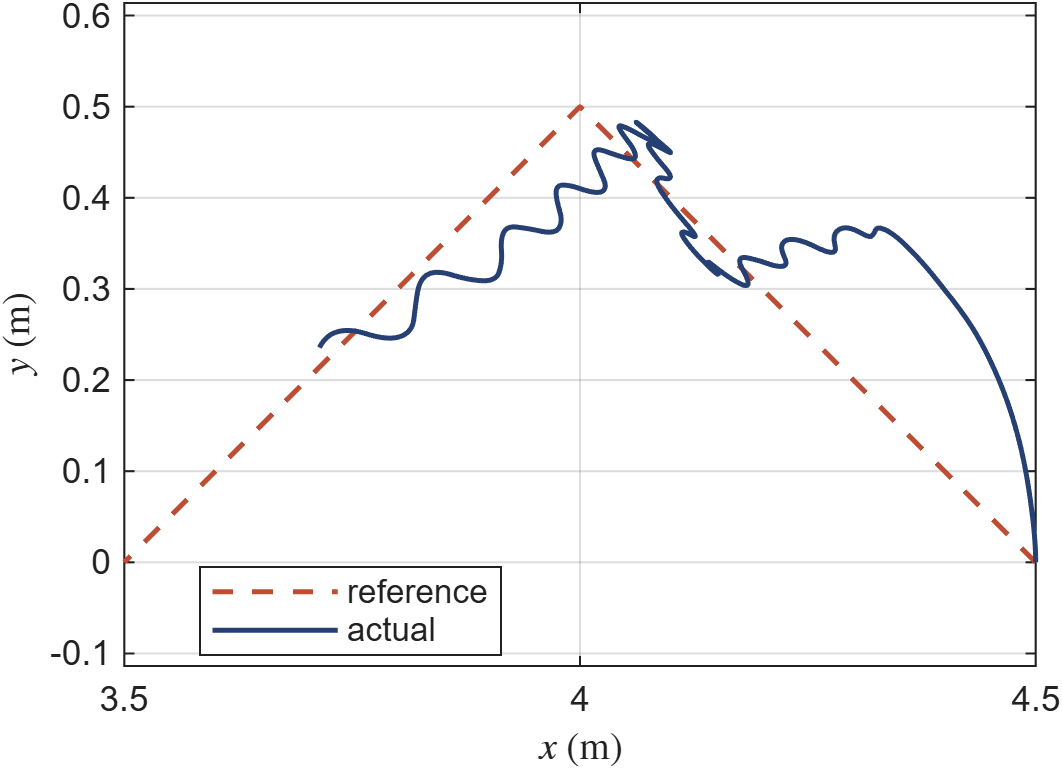
\includegraphics[width=\linewidth]{Figures/rampe_1.png}
        \caption{PPO (Default)}
        \label{fig:r_traj_default}
    \end{subfigure}
    \hfill
    \begin{subfigure}{0.48\textwidth}
        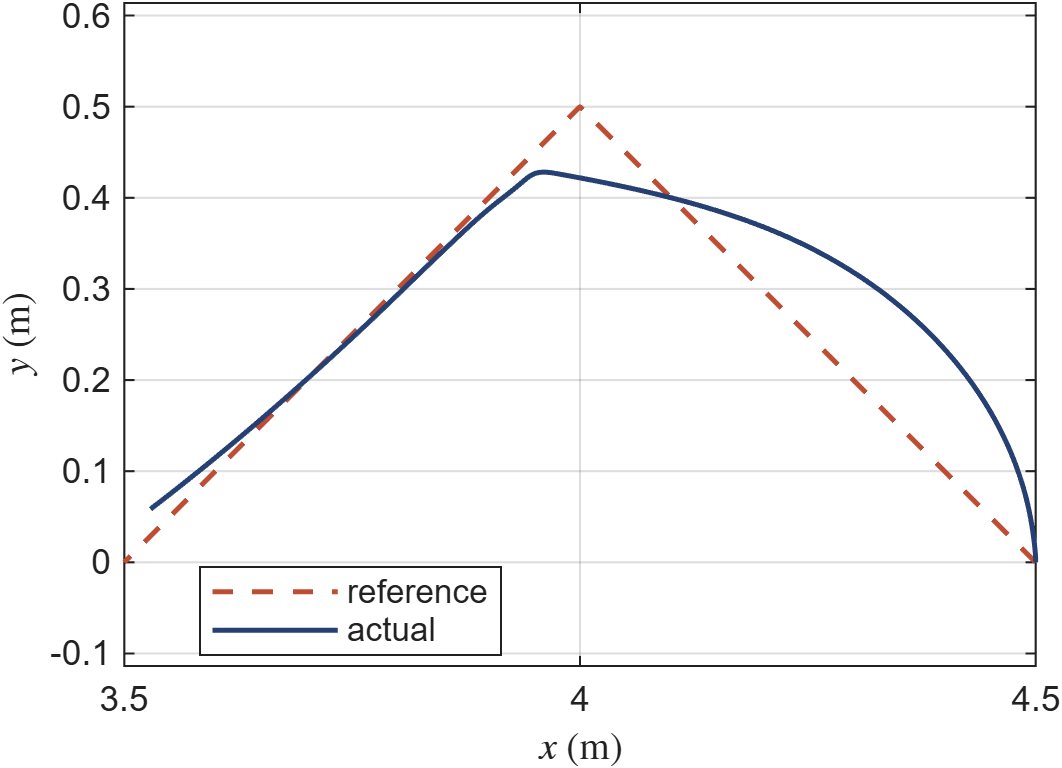
\includegraphics[width=\linewidth]{Figures/rampe_opt_1.png}
        \caption{PPO (Optimized)}
        \label{fig:r_traj_opt}
    \end{subfigure}
    \caption{Target/actual comparison of the \DIFdelbeginFL \DIFdelFL{ramp }\DIFdelendFL \DIFaddbeginFL \DIFaddFL{piecewise-linear }\DIFaddendFL end-effector trajectory in the XY plane.}
    \label{fig:r_trajektorie_xy_compare}
\end{figure*}

\begin{figure*}[!t]
    \centering
    \begin{subfigure}{0.48\textwidth}
        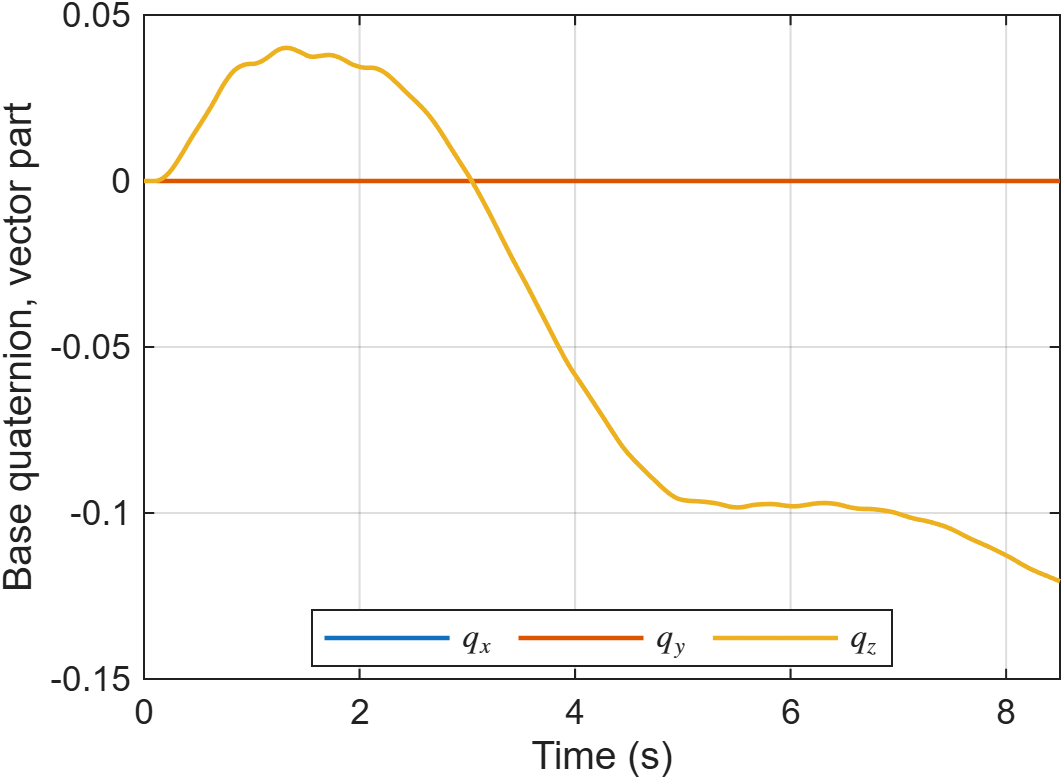
\includegraphics[width=\linewidth]{Figures/basis_ori_1.png}
        \caption{PPO (Default)}
        \label{fig:r_basis_default}
    \end{subfigure}
    \hfill
    \begin{subfigure}{0.48\textwidth}
        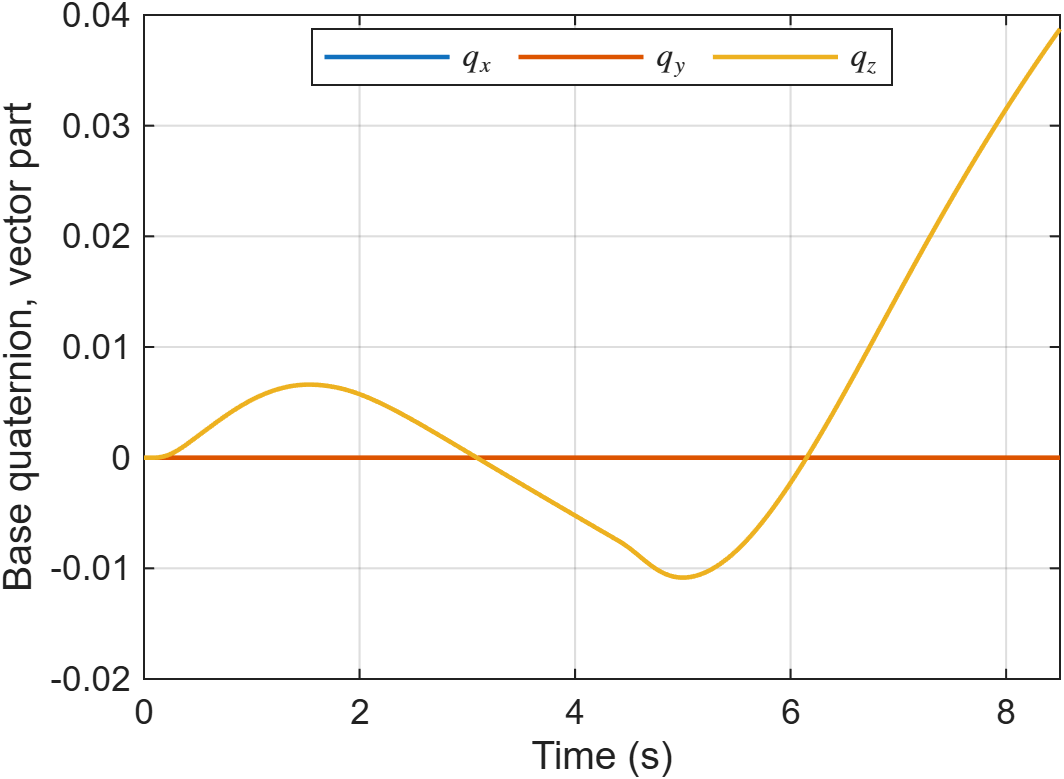
\includegraphics[width=\linewidth]{Figures/basis_ori_opt_1.png}
        \caption{PPO (Optimized)}
        \label{fig:r_basis_opt}
    \end{subfigure}
    \caption{\DIFdelbeginFL \DIFdelFL{Course }\DIFdelendFL \DIFaddbeginFL \DIFaddFL{Time evolution }\DIFaddendFL of \DIFaddbeginFL \DIFaddFL{the }\DIFaddendFL base orientation (quaternion components) during a test episode with \DIFdelbeginFL \DIFdelFL{ramp }\DIFdelendFL \DIFaddbeginFL \DIFaddFL{a piecewise-linear }\DIFaddendFL trajectory.}
    \label{fig:r_basis_orientation_compare}
\end{figure*}
\DIFdelbegin %DIFDELCMD < \noindent
%DIFDELCMD < %%%
\DIFdel{Results: }\DIFdelend \DIFaddbegin \textbf{\DIFadd{Results.}} \DIFaddend Table~\ref{tab:ppo_linear_kpi} reports the KPI averages over \DIFdelbegin \DIFdel{$N_{eval}=30$ }\DIFdelend \DIFaddbegin \DIFadd{$N_{\mathrm{eval}} = 30$ }\DIFaddend evaluation episodes for PPO with the default \DIFdelbegin \DIFdel{configuration }\DIFdelend and the optimized \DIFdelbegin \DIFdel{configuration, now tested }\DIFdelend \DIFaddbegin \DIFadd{configurations }\DIFaddend on the piecewise-linear reference. The optimized PPO \DIFdelbegin \DIFdel{improves overall task success (K1 increases from $-0.4565$ to $-0.2977$}\DIFdelend \DIFaddbegin \DIFadd{increases the episodic return ($K_1$, $-0.4565 \to -0.2977$}\DIFaddend ), reduces \DIFaddbegin \DIFadd{the }\DIFaddend base attitude disturbance (\DIFdelbegin \DIFdel{K4 decreases by $\approx 44\%$) (}\DIFdelend \DIFaddbegin \DIFadd{$K_4$ decreases by approximately $44\%$, }\DIFaddend see~\autoref{fig:r_basis_orientation_compare}), \DIFdelbegin \DIFdel{lowers }\DIFdelend \DIFaddbegin \DIFadd{reduces the }\DIFaddend residual base angular velocity (\DIFdelbegin \DIFdel{K8 decreases by $\approx 15\%$}\DIFdelend \DIFaddbegin \DIFadd{$K_8$ decreases by approximately $15\%$}\DIFaddend ), and \DIFdelbegin \DIFdel{significantly reduces }\DIFdelend \DIFaddbegin \DIFadd{reduces the }\DIFaddend energy consumption (\DIFdelbegin \DIFdel{K9 decreases by $\approx 35\%$}\DIFdelend \DIFaddbegin \DIFadd{$K_9$ decreases by approximately $35\%$}\DIFaddend ). The mean and peak \DIFdelbegin \DIFdel{end-effector }\DIFdelend tracking errors (\DIFdelbegin \DIFdel{K2 and K3) remain almost unchanged}\DIFdelend \DIFaddbegin \DIFadd{$K_2$ and $K_3$) remain close to those of the default configuration}\DIFaddend , with a \DIFdelbegin \DIFdel{slight improvement 
in }\DIFdelend \DIFaddbegin \DIFadd{small reduction of }\DIFaddend the mean error (see~\autoref{fig:r_trajektorie_xy_compare}). \DIFdelbegin \DIFdel{However, the }\DIFdelend \DIFaddbegin \DIFadd{The }\DIFaddend control smoothness metric \DIFdelbegin \DIFdel{(K7) becomes worse than }\DIFdelend \DIFaddbegin \DIFadd{$K_7$, however, is worse than for }\DIFaddend the default PPO. This \DIFdelbegin \DIFdel{suggests }\DIFdelend \DIFaddbegin \DIFadd{indicates }\DIFaddend that the hyperparameter \DIFdelbegin \DIFdel{optimization (highly beneficial }\DIFdelend \DIFaddbegin \DIFadd{configuration tuned }\DIFaddend for circular tracking \DIFdelbegin \DIFdel{) 
}\DIFdelend does not fully transfer to piecewise-linear \DIFdelbegin \DIFdel{motion profiles. A straightforward }\DIFdelend \DIFaddbegin \DIFadd{references. A direct }\DIFaddend mitigation is to include a mixture of reference types (circular, linear\DIFdelbegin \DIFdel{segments}\DIFdelend , and hybrid trajectories) during training \DIFdelbegin \DIFdel{(or during hyperparameter search) to explicitly optimize for trajectory generalization}\DIFdelend \DIFaddbegin \DIFadd{or during the hyperparameter search}\DIFaddend .

\begin{table}[!b]
\centering
\caption{Generalization test on a piecewise-linear end-effector trajectory (two-segment \DIFdelbeginFL \DIFdelFL{ramp}\DIFdelendFL \DIFaddbeginFL \DIFaddFL{path}\DIFaddendFL ). Values are 
averaged over $N_{eval}=30$ episodes. Bold indicates the better value according to the KPI definition (K1 higher is better\DIFdelbeginFL \DIFdelFL{; }\DIFdelendFL \DIFaddbeginFL \DIFaddFL{, }\DIFaddendFL K2--K9 lower is better).}
\label{tab:ppo_linear_kpi}
\renewcommand{\arraystretch}{1.2}
\setlength{\tabcolsep}{3pt}
\begin{tabular}{lcc}
\toprule
\textbf{Metric (KPI)} & \textbf{PPO (Default)} & \textbf{PPO (Optimized)} \\
\midrule
Mean Episodic Reward (K1)            & $-0.4565$ & $\mathbf{-0.2977}$ \\
Mean Squared EE Position Error (K2)  & 0.0078 & \textbf{0.0070} \\
Max EE Position Error (K3)           & 0.2037 & \textbf{0.2036} \\
Mean Base Orientation Error (K4)     & 0.0412 & \textbf{0.0231} \\
Collision Rate (K5)                 & 0 & 0 \\
Joint Limit Violation Rate (K6)     & 0 & 0 \\
Control Smoothness (K7, jerk)       & \textbf{0.5520} & 0.6839 \\
Mean Base Angular Velocity (K8)      & 0.0399 & \textbf{0.0339} \\
Energy Consumption (K9)              & 7.7144 & \textbf{5.0341} \\
\bottomrule
\end{tabular}
\end{table}


Both the circular and \DIFaddbegin \DIFadd{the }\DIFaddend piecewise-linear evaluations \DIFdelbegin \DIFdel{validate the approach }\DIFdelend \DIFaddbegin \DIFadd{support the use }\DIFaddend of systematic hyperparameter tuning and \DIFdelbegin \DIFdel{network tailoring }\DIFdelend \DIFaddbegin \DIFadd{tailored network design }\DIFaddend for safety-critical \DIFdelbegin \DIFdel{space robot control, while also revealing }\DIFdelend \DIFaddbegin \DIFadd{space-robot control. The piecewise-linear results also show }\DIFaddend that trajectory-specific \DIFdelbegin \DIFdel{optimization may be needed for optimal generalization}\DIFdelend \DIFaddbegin \DIFadd{tuning may be required to maintain control smoothness across reference geometries}\DIFaddend .

\DIFdelbegin \DIFdel{In the next section , we will discuss the broader implicationsof these results}\DIFdelend \DIFaddbegin \DIFadd{The following section discusses the implications}\DIFaddend , limitations, and future \DIFdelbegin \DIFdel{avenues to bring this work closer to }\DIFdelend \DIFaddbegin \DIFadd{steps toward }\DIFaddend deployment on physical testbeds for space robotics.

\section{Discussion and Conclusion}
This work has \DIFdelbegin \DIFdel{presented a comprehensive study on applying }\DIFdelend \DIFaddbegin \DIFadd{investigated the application of }\DIFaddend continuous deep reinforcement learning to the control of a free-floating space robotic arm, with an emphasis on safety and performance. The results \DIFdelbegin \DIFdel{demonstrate }\DIFdelend \DIFaddbegin \DIFadd{show }\DIFaddend that an RL-based controller can \DIFdelbegin \DIFdel{successfully handle the challenging
}\DIFdelend \DIFaddbegin \DIFadd{perform the considered }\DIFaddend manipulation task in \DIFdelbegin \DIFdel{a space environment , achieving high trajectory tracking accuracy while keeping
the spacecraft base disturbance to a minimum. The learned agent (especially the optimized PPO policy) was able to coordinate the arm motions in such a way that the }\DIFdelend \DIFaddbegin \DIFadd{the simulated space environment under the stated assumptions. The optimized PPO agent yields a mean squared }\DIFaddend end-effector \DIFdelbegin \DIFdel{closely followed
the desired path and the base’s unintended motions were small and within acceptable bounds, a key
requirement for on-orbit operations. The training process exhibited the typical behavior of RL: an
initial exploration phase where performance was poor (and the agent occasionally triggered safety mechanisms), followed by steady improvement as the agent learned from experience, and finally a
convergence to a stable policy indicated by decreasing variance in returns. The decreasing
variability of the episodic reward and error metrics suggests that the agent’s behavior became reliably
repeatable and less stochastic as it honed in on an optimal strategy }\DIFdelend \DIFaddbegin \DIFadd{tracking error of $K_2 = 0.0083$, a reduction of $67.7\%$ relative to the default configuration ($K_2 = 0.0257$). The mean base-orientation error decreases by a factor of approximately three ($K_4$, $0.0667 \to 0.022$), and the mean base angular velocity is halved ($K_8$, $0.095\,\mathrm{rad/s} \to 0.050\,\mathrm{rad/s}$). No safety violations were recorded over the 30 evaluation episodes ($K_5 = K_6 = 0$), compared with a $5.1\%$ joint-limit violation rate for the default configuration. Torque smoothness improves by $48.5\%$ ($K_7$) and energy consumption decreases by $16\%$ ($K_9$). These effects are observed together in the reported evaluation rather than as an apparent trade-off between the selected objectives }\DIFaddend \cite{b1,b7}.

\DIFdelbegin \DIFdel{One notable achievement is that the agent can generalize to different initial conditions (within the
distribution it was trained on ). We tested the final PPO agent on various starting arm configurations and
positions along the trajectory. It consistently managed to guide the }\DIFdelend \DIFaddbegin \DIFadd{An additional evaluation was carried out on a piecewise-linear }\DIFaddend end-effector \DIFdelbegin \DIFdel{to the circle and then
track it, as long as those initial states were within the training range. This indicates that the policy is
not simply memorizing a sequence of actions, but truly learning a feedback control law that is robust to
moderate variations in the initial state. However, this generalization only holds within the space of
states it experienced. Drastic changes (like a completely different trajectory or a very different initial
base orientation) were not tested and would require either retraining or additional training with such
scenarios (perhaps via domain randomization \mbox{%DIFAUXCMD
\cite{b8}}\hskip0pt%DIFAUXCMD
)}\DIFdelend \DIFaddbegin \DIFadd{reference to assess trajectory generalization. The optimized PPO agent outperforms the default configuration on most metrics, increasing the return $K_1$ from $-0.4565$ to $-0.2977$, reducing the base-orientation error $K_4$ by $44\%$, and reducing the energy $K_9$ by $35\%$, which indicates partial transfer of the learned policy. The control-smoothness metric $K_7$, however, is worse than for the default configuration, showing that the hyperparameter configuration tuned for circular tracking does not fully transfer to piecewise-linear references. This motivates either trajectory-diverse training or trajectory-specific tuning to support generalization across reference geometries \mbox{%DIFAUXCMD
\cite{b8}}\hskip0pt%DIFAUXCMD
}\DIFaddend .

\textbf{Practical Implications\DIFdelbegin \DIFdel{:}\DIFdelend \DIFaddbegin \DIFadd{.}\DIFaddend } The \DIFdelbegin \DIFdel{success of PPO (and TRPO ) in this domain suggests that policy gradient
methods are well-suited for complex, }\DIFdelend \DIFaddbegin \DIFadd{performance of PPO and TRPO on this task indicates that policy-gradient methods with constrained updates are suitable candidates for }\DIFaddend continuous control tasks with \DIFdelbegin \DIFdel{coupled dynamics }\DIFdelend \DIFaddbegin \DIFadd{strong dynamic coupling }\DIFaddend and safety constraints. \DIFdelbegin \DIFdel{In particular, PPO’s ability to handle continuous action spaces and its stable update rule
(}\DIFdelend \DIFaddbegin \DIFadd{The }\DIFaddend clipped surrogate objective \DIFdelbegin \DIFdel{) made it robust in the face of the highly nonlinear dynamics of the }\DIFdelend \DIFaddbegin \DIFadd{of PPO provides bounded policy updates under the nonlinear }\DIFaddend free-floating \DIFdelbegin \DIFdel{robot}\DIFdelend \DIFaddbegin \DIFadd{dynamics}\DIFaddend . The integrated safety components (collision \DIFdelbegin \DIFdel{avoidance, etc.) effectively acted as a form of
“shielding” during training, they prevented the agent from exploring disastrously unsafe actions by
cutting those episodes short \mbox{%DIFAUXCMD
\cite{b15,b23,b22}}\hskip0pt%DIFAUXCMD
. This, combined }\DIFdelend \DIFaddbegin \DIFadd{monitor, joint-limit assertion, torque-bound verification) act as a runtime shield during training. They terminate episodes in which the policy would violate a monitored constraint and apply a terminal penalty \mbox{%DIFAUXCMD
\cite{b15,b23,b22}}\hskip0pt%DIFAUXCMD
. Combined }\DIFaddend with the penalty-driven \DIFdelbegin \DIFdel{learning, means the final policy inherently respects those constraints (since it learned quickly that violating them yields no
reward). For real missions, this is very promising: it implies we can embed safety checks }\DIFdelend \DIFaddbegin \DIFadd{reward, this leads to a final policy that respects the monitored constraints in the reported evaluation. For deployment on a physical system, this suggests that safety checks embedded }\DIFaddend in the training simulator \DIFdelbegin \DIFdel{and reasonably expect the trained policy to abide by them when deployed (assuming the real
system is }\DIFdelend \DIFaddbegin \DIFadd{may remain useful at runtime, provided that the deployed system stays }\DIFaddend within the simulator\DIFdelbegin \DIFdel{’s fidelity ) }\DIFdelend \DIFaddbegin \DIFadd{'s fidelity range }\DIFaddend \cite{b22,b24}.


\textbf{Limitations and Future Work\DIFdelbegin \DIFdel{:}\DIFdelend \DIFaddbegin \DIFadd{.}\DIFaddend }
Several limitations should be acknowledged. First, a \emph{sim-to-real gap} remains\DIFdelbegin \DIFdel{: unmodeled effects such as flexible dynamics, 
}\DIFdelend \DIFaddbegin \DIFadd{. Beyond the idealizing assumptions stated in }\autoref{sec:sim} \DIFadd{(no }\DIFaddend sensor noise, \DIFdelbegin \DIFdel{actuator latency, and external disturbances(e.g., gravity gradients, magnetic torques)could degrade real-world performance~}\DIFdelend \DIFaddbegin \DIFadd{no latency, rigid body model, no external disturbances), real deployment introduces additional challenges. These are (a)~}\emph{\DIFadd{domain shift}} \DIFadd{due to inaccuracies in the identified mass and inertia parameters, joint friction, and link flexibility not captured in the URDF model, (b)~}\emph{\DIFadd{onboard compute constraints}}\DIFadd{, as the learned neural network policy must execute in real time on embedded space-qualified hardware (typically ARM-based processors with limited floating-point throughput), whereas training was performed on a workstation-class CPU, and (c)~}\emph{\DIFadd{sensor-actuator latency}}\DIFadd{, where non-negligible delays between state measurement and torque application can destabilize a policy trained under the zero-latency assumption. Mitigating these effects requires domain randomization over simulation parameters, latency injection during training, and ultimately hardware-in-the-loop (HIL) validation~}\DIFaddend \cite{b8,b22}.
Second, the RL agent exhibits \emph{hyperparameter sensitivity}\DIFdelbegin \DIFdel{---the }\DIFdelend \DIFaddbegin \DIFadd{. The }\DIFaddend tuned PPO configuration is task-specific and may require re-tuning for different
trajectories or mission scenarios. Third, the \emph{state representation} was manually designed\DIFdelbegin \DIFdel{; learned }\DIFdelend \DIFaddbegin \DIFadd{. Learned }\DIFaddend representations or recurrent architectures (LSTM)
might improve performance under partial observability. Fourth, the \emph{safety monitoring} covers targeted critical properties but does not constitute
exhaustive formal verification of the full mission~\cite{b5,b22}. Finally, \emph{no hardware testing} was performed\DIFdelbegin \DIFdel{; real-time }\DIFdelend \DIFaddbegin \DIFadd{. Real-time }\DIFaddend computation limits,
communication delays, and physical interactions remain to be validated \DIFaddbegin \DIFadd{on physical testbeds}\DIFaddend .

Future work should address these gaps \DIFdelbegin \DIFdel{through: }\DIFdelend \DIFaddbegin \DIFadd{in several directions. These are }\DIFaddend (i)~domain randomization over simulation parameters \DIFdelbegin \DIFdel{to improve robustness for }\DIFdelend \DIFaddbegin \DIFadd{and latency injection to improve }\DIFaddend sim-to-real \DIFdelbegin \DIFdel{transfer~\mbox{%DIFAUXCMD
\cite{b8} }\hskip0pt%DIFAUXCMD
; (}\DIFdelend \DIFaddbegin \DIFadd{robustness~\mbox{%DIFAUXCMD
\cite{b8} }\hskip0pt%DIFAUXCMD
(see \mbox{%DIFAUXCMD
\cref{fig:oos}}\hskip0pt%DIFAUXCMD
), (}\DIFaddend ii)~extension to more complex tasks such as dual-arm coordination, on-orbit assembly, or active debris removal\DIFdelbegin \DIFdel{; }\DIFdelend \DIFaddbegin \DIFadd{, }\DIFaddend (iii)~advanced
RL architectures (recurrent policies, attention mechanisms) and safe RL algorithms with explicit constraint handling via Lagrange multipliers
or barrier functions~\cite{b22,b24,b23,b34}\DIFdelbegin \DIFdel{; }\DIFdelend \DIFaddbegin \DIFadd{, }\DIFaddend and (iv)~hardware-in-the-loop validation \DIFdelbegin \DIFdel{e.g. on our }\DIFdelend \DIFaddbegin \DIFadd{on the authors' }\DIFaddend testbed for In-Space Robotized Services (IROS) with virtually simulated microgravity and predicted energy consumption (see \DIFdelbegin \DIFdel{\mbox{%DIFAUXCMD
\cref{fig:physicaltestbed}}\hskip0pt%DIFAUXCMD
}\DIFdelend \DIFaddbegin \DIFadd{\mbox{%DIFAUXCMD
\cref{fig:oos}}\hskip0pt%DIFAUXCMD
}\DIFaddend ).


\textbf{Conclusion\DIFdelbegin \DIFdel{:}\DIFdelend \DIFaddbegin \DIFadd{.}\DIFaddend } \DIFdelbegin \DIFdel{In conclusion, this research demonstrates a viable framework for applying }\DIFdelend \DIFaddbegin \DIFadd{This work has presented a framework that combines }\DIFaddend deep reinforcement learning\DIFdelbegin \DIFdel{to complex space robotic systems. We showed that by combining high-fidelity
modeling, multiple RL algorithm evaluations, and integrated formal safety checks, one can develop a control policy that achieves high precision and reliability in a challenging }\DIFdelend \DIFaddbegin \DIFadd{, multibody simulation, and formal-methods-based safety monitoring for Cartesian path tracking of a }\DIFaddend free-floating \DIFdelbegin \DIFdel{manipulation
task. The comparative analysis revealed PPO as an effective solution, and further optimizations
}\DIFdelend \DIFaddbegin \DIFadd{space robot. A comparison of six continuous-action RL algorithms under unified conditions identified PPO as the algorithm with the most favorable trade-off between tracking accuracy, base disturbance, and training stability for the considered task. Subsequent hyperparameter tuning and network tailoring of the PPO agent }\DIFaddend yielded a policy that\DIFdelbegin \DIFdel{meets stringent trajectory and safety requirements. Importantly, the use of formal
methods alongside RL is a novel contribution, it addresses the }\DIFdelend \DIFaddbegin \DIFadd{, relative to the default PPO configuration, reduces the tracking error by $67.7\%$, reduces the base-orientation error by a factor of approximately three, shows no joint-limit or collision violations over 30 evaluation episodes, and reduces the energy consumption by $16\%$. The integration
of monitored safety constraints and torque-bound verification into the training loop helped keep these results
within the defined safety envelope, addressing part of the }\DIFaddend typical black-box
nature of learned controllers\DIFdelbegin \DIFdel{by adding verifiable guarantees for certain behaviors. This synergy of model-based and
data-driven methods is very promising for space systems, where safety cannot be compromised}\DIFdelend . \DIFaddbegin \DIFadd{These findings, grounded in quantitative experimental evidence,
support further investigation of safety-augmented deep RL for safety-critical space manipulation tasks.
}\DIFaddend 



The \DIFdelbegin \DIFdel{work also provides insights into }\DIFdelend \DIFaddbegin \DIFadd{results also illustrate }\DIFaddend the influence of algorithm choice and parameter tuning on learning performance for \DIFdelbegin \DIFdel{physical systems. Our findings reinforce the notion that there is no one-size-fits-all in RL , careful selection and tuning of the agent (and network structure) can significantly
impact the outcome, even more so than we might expect from generic benchmarks. For practitioners,
this means that investing time in benchmarking algorithms (as we did) can pay off in identifying the \mbox{right approach for the problem at hand.}
}\DIFdelend \DIFaddbegin \DIFadd{the considered task. They support the view that no single RL algorithm is uniformly best across applications: under unified conditions, the choice of algorithm, network architecture, and hyperparameter setting visibly affects the achieved tracking accuracy and base stability. Systematic benchmarking of candidate algorithms is therefore a practical step in the selection of an appropriate RL controller for a given task.
}\DIFaddend 

\DIFdelbegin \DIFdel{Finally, while challenges }\DIFdelend \DIFaddbegin \DIFadd{While several open problems }\DIFaddend remain for real-world deployment, \DIFdelbegin \DIFdel{this study lays a foundation. It suggests that
future space robots, tasked with servicingsatellites, assembling structures, or handling space debris }\DIFdelend \DIFaddbegin \DIFadd{the proposed framework provides a basis for further investigation. Possible application areas include satellite servicing}\DIFaddend , \DIFdelbegin \DIFdel{could employ }\DIFdelend \DIFaddbegin \DIFadd{on-orbit assembly, and active debris removal, where }\DIFaddend learning-based controllers \DIFdelbegin \DIFdel{that adapt to complex dynamics and uncertainties, all while
operating safely within predefined limits. We envision an architecture where an RL policy drives the
robot’s motions, supervised by a layer of formal logic }\DIFdelend \DIFaddbegin \DIFadd{can adapt to uncertain dynamics within predefined operational limits. The combination of an RL policy with a separate runtime layer }\DIFaddend that monitors and\DIFdelbegin \DIFdel{vetoes any unacceptable
actions (though, ideally, the policy has learned not to propose such actions in the first place). Such
an approach could provide the flexibility and efficiency of learned behaviors with the trust and
guarantee of model-based safety, a combination well-suited to the unforgiving environment of space }\DIFdelend \DIFaddbegin \DIFadd{, where required, overrides commands violating the specified constraints is one realization of such an architecture. In this combination, the learned policy provides adaptability, while the monitoring layer enforces the specified safety-critical properties~}\DIFaddend \cite{b1,b23}.

%DIF > \begin{figure}[!t]
%DIF > 	\centering
%DIF > 	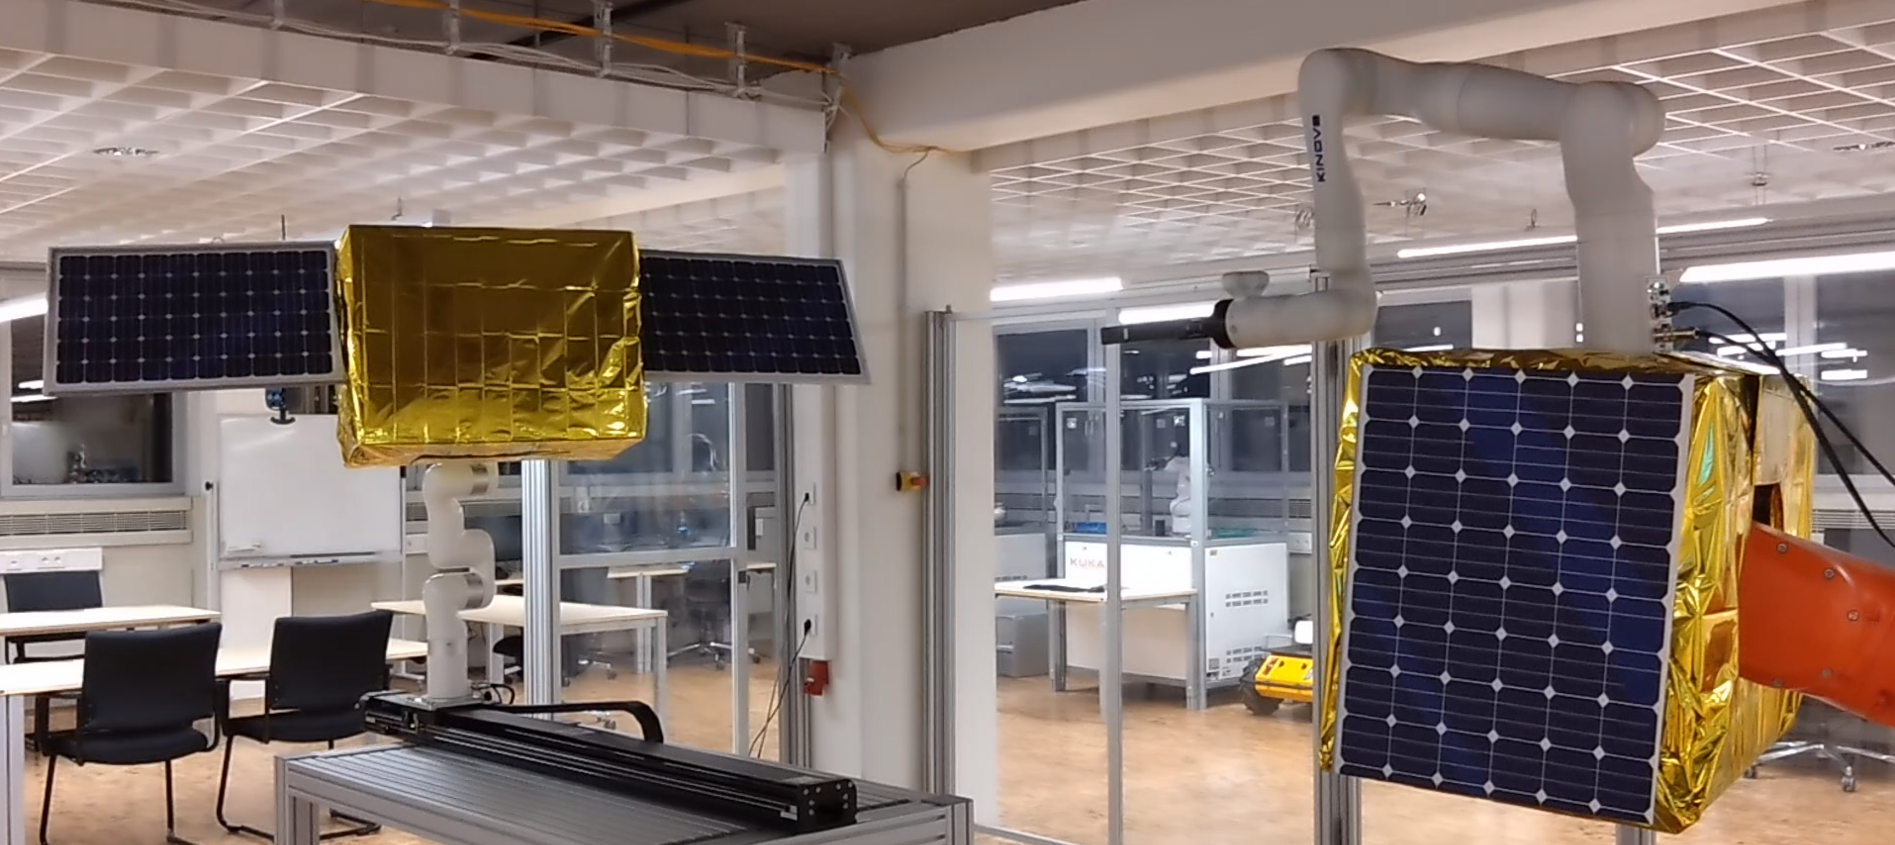
\includegraphics[width=0.8\linewidth]{Figures/testbed.png}
%DIF > 	\caption{Our testbed for In-Space Robotized Services.}
%DIF > 	\label{fig:physicaltestbed}
%DIF > \end{figure}
\DIFaddbegin 

\DIFaddend \begin{figure}[!t]
	\centering
	\DIFdelbeginFL %DIFDELCMD < 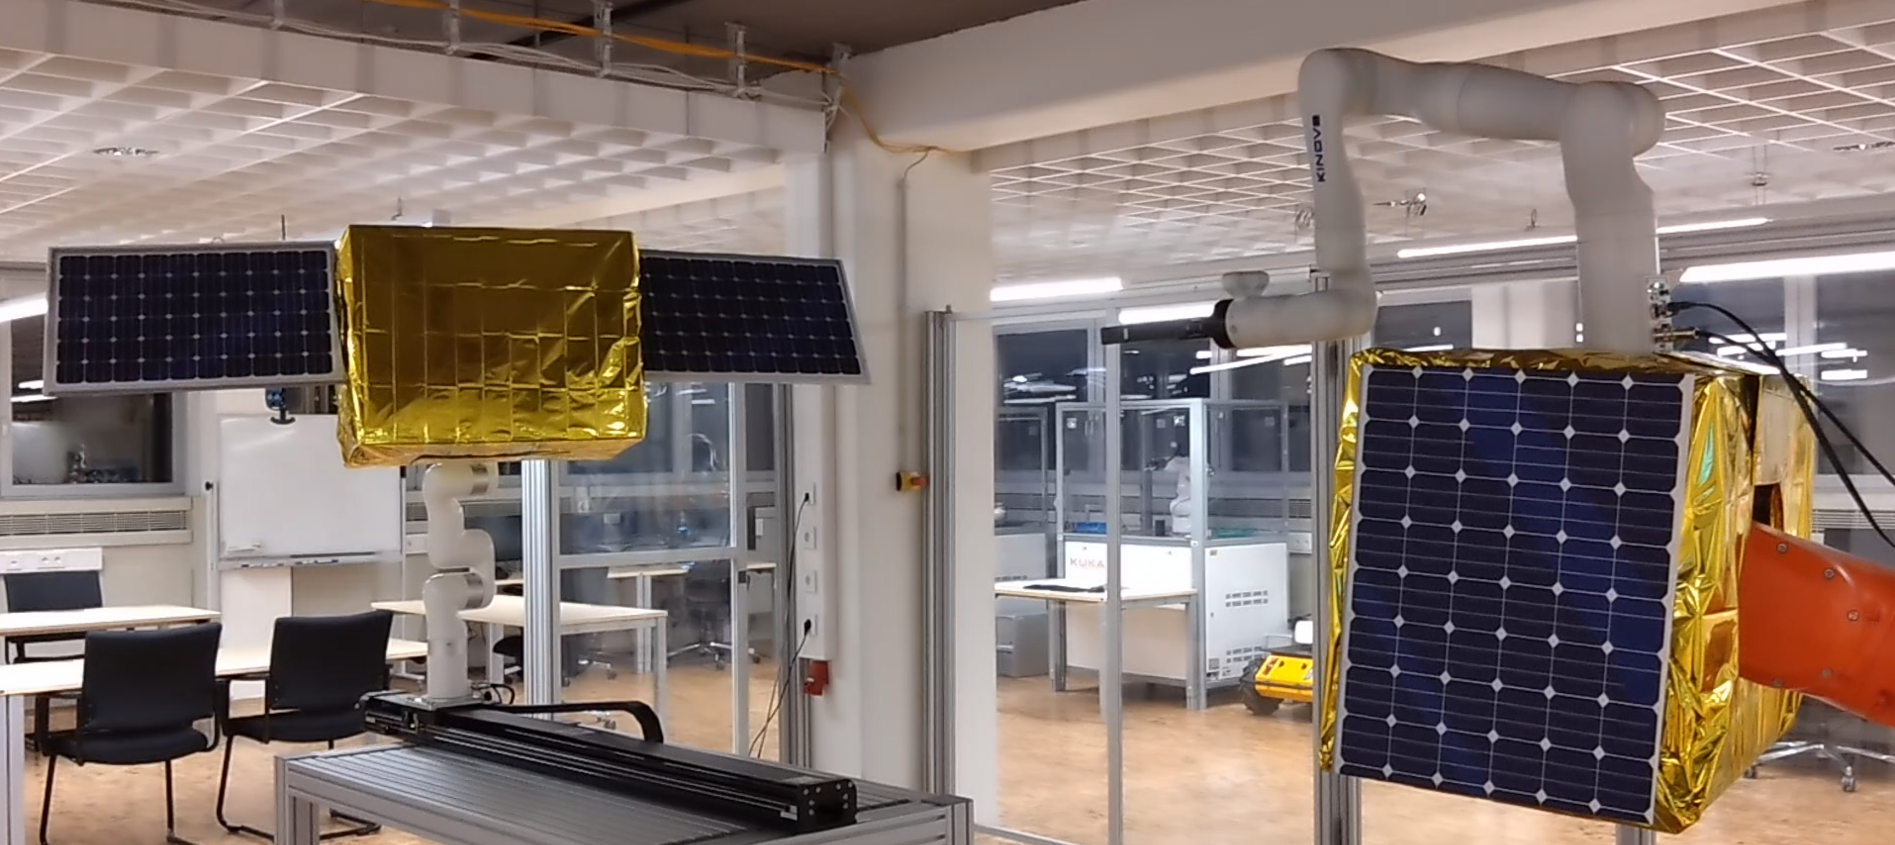
\includegraphics[width=0.8\linewidth]{Figures/testbed.png}
%DIFDELCMD < 	%%%
\DIFdelendFL \DIFaddbeginFL \begin{subfigure}{0.99\columnwidth}
		\centering
		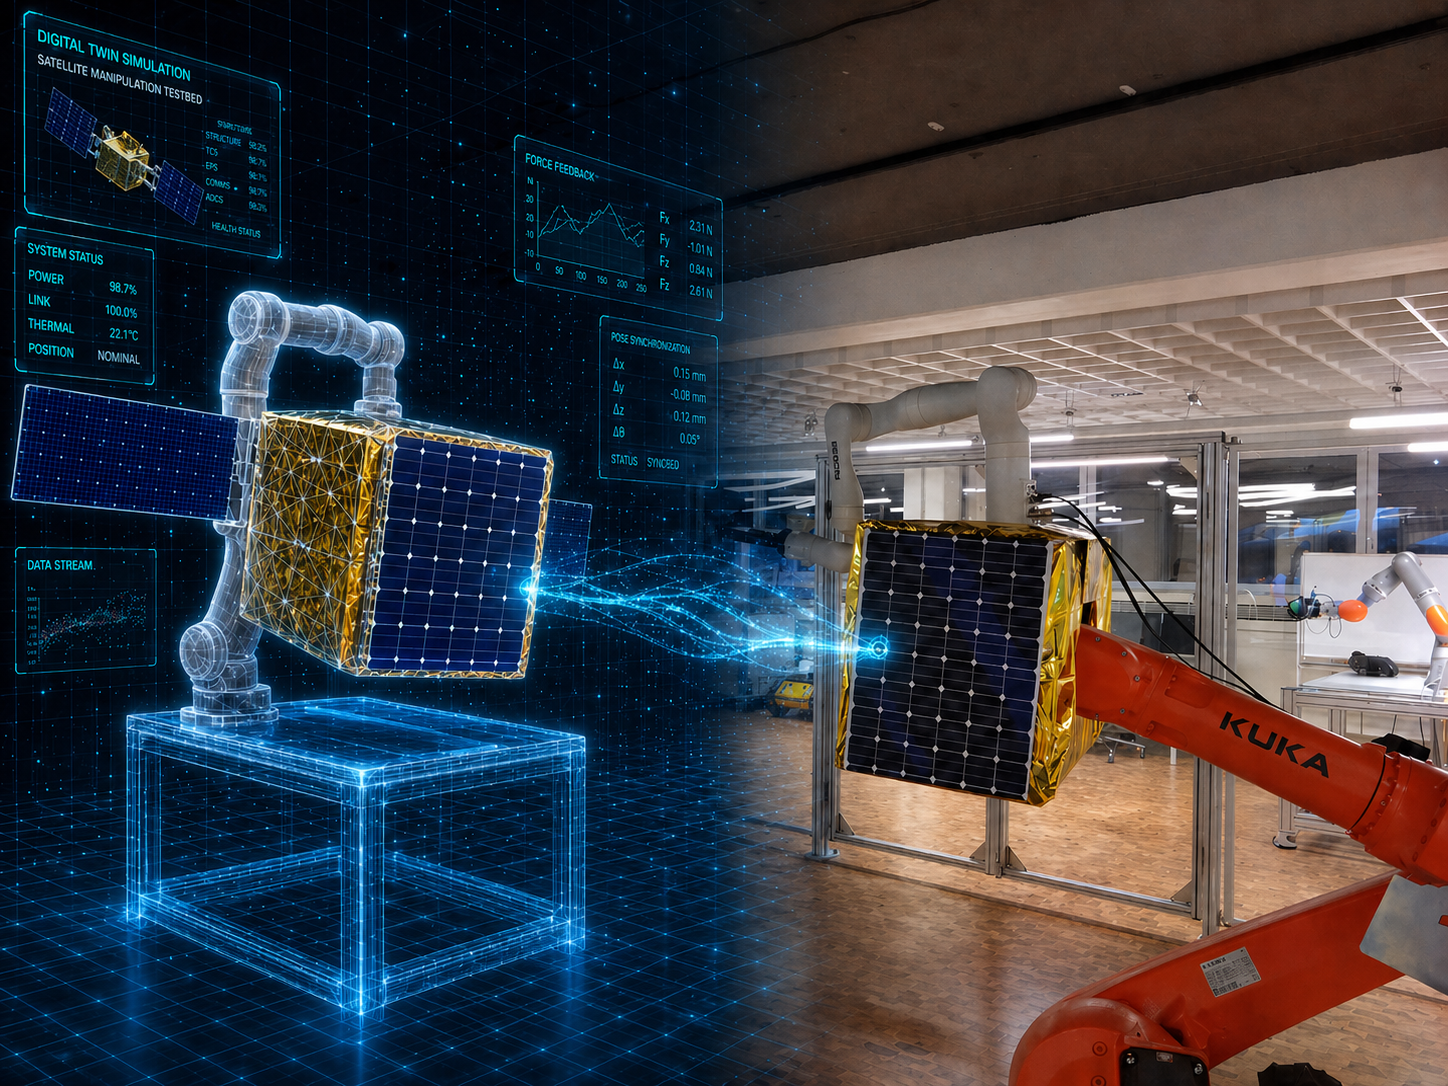
\includegraphics[width=\linewidth]{Figures/oos1.png}
	\end{subfigure}
	\DIFaddendFL \caption{\DIFdelbeginFL \DIFdelFL{Our testbed }\DIFdelendFL \DIFaddbeginFL \DIFaddFL{Gradual hybrid testbeds integrate AI-driven digital twins (left) with physical robotic systems (right), providing a framework }\DIFaddendFL for \DIFdelbeginFL \DIFdelFL{In-Space Robotized Services}\DIFdelendFL \DIFaddbeginFL \DIFaddFL{studying policy optimization and domain-randomization strategies for sim-to-real transfer}\DIFaddendFL . \DIFaddbeginFL \DIFaddFL{Illustration created using a picture of the physical setup at Frankfurt University of Applied Sciences
		and with the help of GPT-Image-2.}\DIFaddendFL }
	\DIFdelbeginFL %DIFDELCMD < \label{fig:physicaltestbed}
%DIFDELCMD < %%%
\DIFdelendFL \DIFaddbeginFL \label{fig:oos}
\DIFaddendFL \end{figure}

\DIFdelbegin \DIFdel{Ultimately, our work demonstrates a step in that direction, confirming that with the right algorithms
and safeguards, “autonomous learning-based control” can be a powerful paradigm for future space
robotic missions. The results encourage continued }\DIFdelend \DIFaddbegin \DIFadd{The present study contributes one step in this direction. Future }\DIFaddend research at the intersection of robotics, reinforcement learning, and formal methods \DIFdelbegin \DIFdel{to further unlock the potential of intelligent space
systems}\DIFdelend \DIFaddbegin \DIFadd{is required to extend the present results to physical deployment and to broader mission scenarios}\DIFaddend .

\section*{Acknowledgment}
The authors used DeepL Translator/Write~\cite{deeplTr,deeplWr} and OpenAI ChatGPT~\cite{openai_chatgpt} solely for language editing and grammar enhancement. 
All technical content and conclusions were created and verified by the authors.

\begin{thebibliography}{00}

\bibitem{b1}
A. Flores-Abad, O. Ma, K. Pham, and S. Ulrich, ``A review of space robotics technologies for on-orbit servicing,'' \emph{Prog. Aerosp. Sci.}, vol.~68, pp. 1--26, 2014, doi: 10.1016/j.paerosci.2014.03.002.



\bibitem{b6}
K. Nanos and E. G. Papadopoulos, ``On the dynamics and control of free-floating space manipulator systems in the presence of angular momentum,'' \emph{Front. Robot. AI}, vol.~4, p.~26, 2017, doi: 10.3389/frobt.2017.00026.



\bibitem{b11}
E. Papadopoulos, I. Kaliakatsos, and D. Psarros, ``Minimum fuel techniques for a space robot simulator with a reaction wheel and PWM thrusters,'' in \emph{Proc. Eur. Control Conf. (ECC)}, 2007, pp. 3391--3398.



\bibitem{b32}
E. Papadopoulos and A. Abu-Abed, ``Design and motion planning for a zero-reaction manipulator,'' in \emph{Proc. IEEE Int. Conf. Robot. Autom. (ICRA)}, 1994, pp. 1554--1559, doi: 10.1109/ROBOT.1994.351367.



\bibitem{muhlbauer2025software}
M. M{\"u}hlbauer, M. Chalon, M. Ulmer, and A. Albu-Sch{\"a}ffer, ``Software for the SpaceDREAM robotic arm,'' in \emph{Proc. IEEE Aerosp. Conf.}, 2025.



\bibitem{rybus2024robotic}
T. Rybus, ``Robotic manipulators for in-orbit servicing and active debris removal: Review and comparison,'' \emph{Prog. Aerosp. Sci.}, vol.~151, p.~104550, 2024.



%\bibitem{maurenbrecher2024robograv}
%H. Maurenbrecher \emph{et al.}, ``RoboGrav---Towards force sensitive space manipulators,'' in \emph{Proc. I-SAIRAS}, 2024.

\bibitem{kaigom2011optimal}
E. Guiffo Kaigom, T. Jung, and J. Roßmann, ``Optimal motion planning of a space robot with base disturbance minimization,'' in \emph{Proc. 11th Symp. Adv. Space Technol. Robot. Autom.}, 2011.

\bibitem{kaigom2025deep}
E. Guiffo Kaigom, ``Deep generative and discriminative digital twin endowed with variational autoencoder for unsupervised predictive thermal condition monitoring of physical robots in Industry 6.0 and Society 6.0,'' \emph{IFAC-PapersOnLine}, vol.~59, pp. 7--12, 2025.

\bibitem{huang2023obstacle}
Z. Huang, G. Chen, Y. Shen, R. Wang, C. Liu, and L. Zhang, ``An obstacle-avoidance motion planning method for redundant space robot via reinforcement learning,'' \emph{Actuators}, vol.~12, no.~2, p.~69, 2023.



\bibitem{al2024reinforcement}
A. Al Ali and Z. Zhu, ``Reinforcement learning for path planning of free-floating space robotic manipulator with collision avoidance and observation noise,'' \emph{Front. Control Eng.}, vol.~5, p.~1394668, 2024.



\bibitem{d2024failure}
M. D'Ambrosio, L. Capra, A. Brandonisio, and M. Lavagna, ``Failure management via deep reinforcement learning for robotic in-orbit servicing,'' in \emph{Proc. SPAICE---1st Joint ESA/IAA Conf. AI Space}, 2024, pp. 335--339.



\bibitem{al2024path}
A. Al Ali, J. Shi, and Z. Zhu, ``Path planning of 6-DOF free-floating space robotic manipulators using reinforcement learning,'' \emph{Acta Astronaut.}, vol.~224, pp. 367--378, 2024.



\bibitem{hu2025deep}
Y. Hu, D. Zhou, W. Yao, X. Shao, and G. Sun, ``Deep reinforcement learning-based trajectory planning with continuous pose representation for 6-DoF free-floating space robot,'' \emph{Aerosp. Sci. Technol.}, p.~110540, 2025.



\bibitem{zhang2025learning}
O. Zhang, Z. Liu, X. Shao, W. Yao, L. Wu, and J. Liu, ``Learning-based task space trajectory planning framework with pre-planning and post-processing for uncertain free-floating space robots,'' \emph{IEEE Trans. Aerosp. Electron. Syst.}, early access, 2025.



\bibitem{wei2025trajectory}
Y. Wei, X. Bai, and H. Lu, ``Trajectory planning of free-floating space robot for non-cooperative tumbling target capture based on deep reinforcement learning,'' \emph{Robotica}, vol.~43, pp. 2674--2692, 2025.



\bibitem{wu2020reinforcement}
Y. Wu, Z. Yu, C. Li, M. He, B. Hua, and Z. Chen, ``Reinforcement learning in dual-arm trajectory planning for a free-floating space robot,'' \emph{Aerosp. Sci. Technol.}, vol.~98, p.~105657, 2020.



\bibitem{b14}
J. Schulman, S. Levine, P. Abbeel, M. Jordan, and P. Moritz, ``Trust region policy optimization,'' in \emph{Proc. Int. Conf. Mach. Learn. (ICML)}, 2015, pp. 1889--1897.



\bibitem{b17}
S. Fujimoto, H. van Hoof, and D. Meger, ``Addressing function approximation error in actor-critic methods,'' in \emph{Proc. Int. Conf. Mach. Learn. (ICML)}, 2018, pp. 1587--1596.



\bibitem{b18}
T. Haarnoja, A. Zhou, P. Abbeel, and S. Levine, ``Soft actor-critic: Off-policy maximum entropy deep reinforcement learning with a stochastic actor,'' in \emph{Proc. Int. Conf. Mach. Learn. (ICML)}, 2018, pp. 1861--1870.



\bibitem{b15}
J. Schulman, F. Wolski, P. Dhariwal, A. Radford, and O. Klimov, ``Proximal policy optimization algorithms,'' arXiv:1707.06347, 2017.



\bibitem{b21}
R. J. Williams, ``Simple statistical gradient-following algorithms for connectionist reinforcement learning,'' \emph{Mach. Learn.}, vol.~8, pp. 229--256, 1992.



\bibitem{b7}
R. S. Sutton and A. G. Barto, \emph{Reinforcement Learning: An Introduction}, 2nd~ed. Cambridge, MA, USA: MIT Press, 2018.



\bibitem{b5}
MathWorks, ``Simulink Design Verifier,'' \DIFdelbegin \DIFdel{The MathWorks, Inc., Natick, MA, USA, }\DIFdelend \DIFaddbegin \DIFadd{MATLAB \& Simulink Documentation, }\DIFaddend 2024. [Online]. Available: \url{https://www.mathworks.com/help/sldv/}



\bibitem{b22}
J. Garc{\'\i}a and F. Fern{\'a}ndez, ``A comprehensive survey on safe reinforcement learning,'' \emph{J. Mach. Learn. Res.}, vol.~16, pp. 1437--1480, 2015.



\bibitem{b23}
M. Alshiekh, R. Bloem, R. Ehlers, B. K{\"o}nighofer, S. Niekum, and U. Topcu, ``Safe reinforcement learning via shielding,'' in \emph{Proc. AAAI Conf. Artif. Intell.}, 2018, pp. 2669--2678.



\bibitem{b25}
Open Robotics, ``URDF (Unified Robot Description Format),'' ROS~2 Documentation, 2024. [Online]. Available: \url{https://docs.ros.org/en/rolling/Tutorials/Intermediate/URDF/URDF-Main.html}



\bibitem{b26}
MathWorks, ``Import URDF models,'' MATLAB \& Simulink Documentation, 2024. [Online]. Available: \url{https://www.mathworks.com/help/sm/ug/urdf-import.html}



\bibitem{b27}
MathWorks, ``smimport---Import a CAD, URDF, or Robotics System Toolbox model,'' MATLAB \& Simulink Documentation, 2024. [Online]. Available: \url{https://www.mathworks.com/help/sm/ref/smimport.html}



\bibitem{b28}
MathWorks, ``Mechanism Configuration,'' MATLAB \& Simulink Documentation, 2024. [Online]. Available: \url{https://www.mathworks.com/help/sm/ref/mechanismconfiguration.html}



\bibitem{b2}
J. Kober, J. A. Bagnell, and J. Peters, ``Reinforcement learning in robotics: A survey,'' \emph{Int. J. Robot. Res.}, vol.~32, no.~11, pp. 1238--1274, 2013.



\bibitem{b24}
J. Achiam, D. Held, A. Tamar, and P. Abbeel, ``Constrained policy optimization,'' in \emph{Proc. Int. Conf. Mach. Learn. (ICML)}, 2017, pp. 22--31.



\bibitem{b34}
A. D. Ames, S. Coogan, M. Egerstedt, G. Notomista, K. Sreenath, and P. Tabuada, ``Control barrier functions: Theory and applications,'' in \emph{Proc. Eur. Control Conf. (ECC)}, 2019, pp. 3420--3431.



\bibitem{leutert2024ai}
F. Leutert \emph{et al.}, ``AI-enabled cyber--physical in-orbit factory---AI approaches based on digital twin technology for robotic small satellite production,'' \emph{Acta Astronaut.}, vol.~217, pp. 1--17, 2024.



\bibitem{muhlbauer2025towards}
M. M{\"u}hlbauer \emph{et al.}, ``Towards an in-orbit cubesat factory,'' in \emph{Proc. 76th Int. Astronaut. Congr. (IAC)}, 2025.



\bibitem{maqbool2025systems}
O. Maqbool and J. Roßmann, ``Systems aware scenario engineering for life cycle-spanning verification and validation of complex CPS,'' Authorea Preprints, 2025. [Online]. Available: \url{https://www.authorea.com}



\bibitem{b9}
J. Virgili-Llop, ``SPART: Spacecraft Robotics Toolkit,'' 2017. [Online]. Available: \url{https://github.com/NPS-SRL/SPART}



\bibitem{b12}
E. Ribeiro, R. Mendes, M. Terra, and V. Grassi, ``Dynamic parameter identification of a 7-DoF lightweight robot manipulator using probabilistic differential optimization,'' in \emph{Proc. IEEE Int. Conf. Syst., Man, Cybern. (SMC)}, 2022, pp. 1917--1923.



\bibitem{b3}
MathWorks, ``6-DOF Joint (Simscape Multibody),'' MATLAB \& Simulink Documentation, 2024. [Online]. Available: \url{https://www.mathworks.com/help/sm/ref/6dofjoint.html}



\bibitem{b31}
MathWorks, ``Spatial Contact Force,'' MATLAB \& Simulink Documentation, 2024. [Online]. Available: \url{https://www.mathworks.com/help/sm/ref/spatialcontactforce.html}



\bibitem{b29}
MathWorks, ``Solver Configuration,'' MATLAB \& Simulink Documentation, 2024. [Online]. Available: \url{https://www.mathworks.com/help/simscape/ref/solverconfiguration.html}



\bibitem{b30}
MathWorks, ``Fixed-step size (fundamental sample time),'' MATLAB \& Simulink Documentation, 2024. [Online]. Available: \url{https://www.mathworks.com/help/simulink/gui/fixedstepsizefundamentalsampletime.html}



\bibitem{b4}
MathWorks, ``Reinforcement Learning Toolbox---rlPPOAgent,'' MATLAB \& Simulink Documentation, 2024. [Online]. Available: \url{https://www.mathworks.com/help/reinforcement-learning/ref/rl.agent.rlppoagent.html}



\bibitem{b16}
T. P. Lillicrap \emph{et al.}, ``Continuous control with deep reinforcement learning,'' in \emph{Proc. Int. Conf. Learn. Represent. (ICLR)}, 2016.



\bibitem{b8}
J. Tobin, R. Fong, A. Ray, J. Schneider, W. Zaremba, and P. Abbeel, ``Domain randomization for transferring deep neural networks from simulation to the real world,'' in \emph{Proc. IEEE/RSJ Int. Conf. Intell. Robots Syst. (IROS)}, 2017, pp. 23--30.


\bibitem{deeplTr}
DeepL SE, ``DeepL Translator,'' [Online]. Available: \url{https://www.deepl.com/de/translator}

\bibitem{deeplWr}
DeepL SE, ``DeepL Write,'' [Online]. Available: \url{https://www.deepl.com/de/write}


\bibitem{openai_chatgpt}
OpenAI, ``ChatGPT,'' [Online]. Available: \url{https://chat.openai.com}



\DIFaddbegin \bibitem{todorov2012mujoco}
\DIFadd{E. Todorov, T. Erez, and Y. Tassa, ``MuJoCo: A physics engine for model-based control,'' in }\emph{\DIFadd{Proc. IEEE/RSJ Int. Conf. Intell. Robots Syst. (IROS)}}\DIFadd{, 2012, pp. 5026--5033.
}



\bibitem{koenig2004gazebo}
\DIFadd{N. Koenig and A. Howard, ``Design and use paradigms for Gazebo, an open-source multi-robot simulator,'' in }\emph{\DIFadd{Proc. IEEE/RSJ Int. Conf. Intell. Robots Syst. (IROS)}}\DIFadd{, vol.~3, 2004, pp. 2149--2154.
}



\bibitem{korber2021comparing}
\DIFadd{M. K\"orber, J. Lange, S. Rediske, S. Steinmann, and R. Gl\"uck, ``Comparing popular simulation environments in the scope of robotics and reinforcement learning,'' arXiv:2103.04616, 2021.
}



\bibitem{collins2021review}
\DIFadd{J. Collins, S. Chand, A. Vanderkop, and D. Howard, ``A review of physics simulators for robotic applications,'' }\emph{\DIFadd{IEEE Access}}\DIFadd{, vol.~9, pp. 51416--51431, 2021.
}



\DIFaddend \end{thebibliography}

\begin{IEEEbiography}[{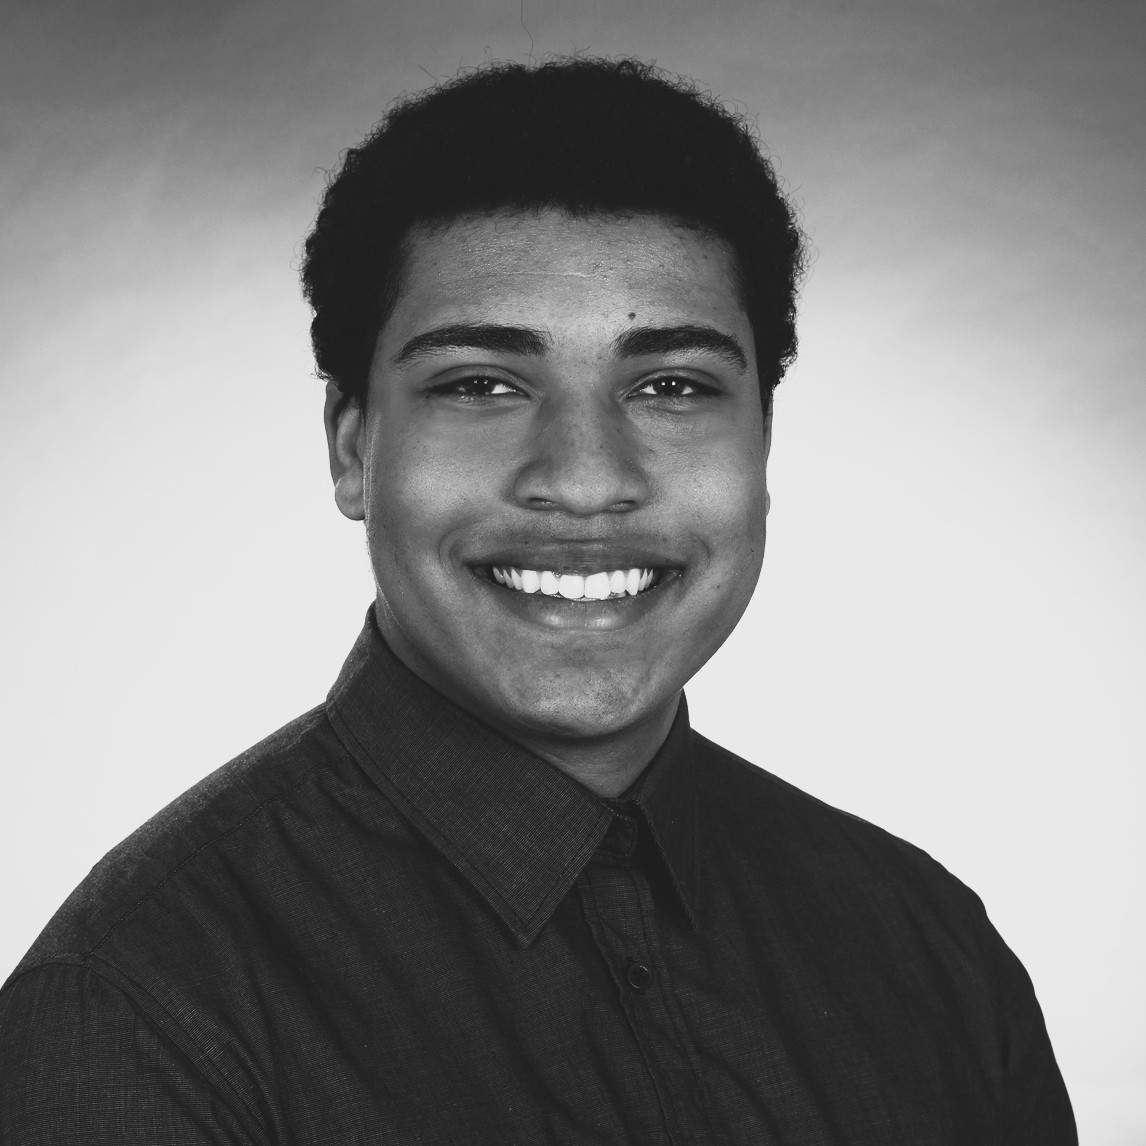
\includegraphics[width=1in,height=1.25in,clip,keepaspectratio]{Figures/Bewerbungsfoto_Ermisch.jpg}}]{Patrick S. Ermisch}
Patrick S. Ermisch was born in Frankfurt am Main, Germany, on December 18, 2002. He received the Abitur degree and 
is currently pursuing the B.Eng. degree in mechatronics at Frankfurt University of Applied Sciences, Frankfurt, 
Germany, with an expected graduation in 2026. His major field of study is mechatronics.

He has gained practical experience through an internship at SEW-EURODRIVE, where he contributed to the further 
development of a mobile application for the manual control of logistics robots. In addition, he worked as a tutor 
for Physics~I and Physics~II and as a student research assistant, supporting research on particle simulation and 
the development of an application for visualization and simulation purposes. His research interests include 
reinforcement learning for robotics, space robotic systems, and simulation-based control methods.

Mr.\ Ermisch has been listed on the Dean’s List of Frankfurt University of Applied Sciences multiple times in 
recognition of his academic performance.
\end{IEEEbiography}



\begin{IEEEbiography}[{
\includegraphics[width=1in,height=1.25in,clip,keepaspectratio]{Figures/egk.jpg}}]{Eric Guiffo Kaigom} was born in Douala, Cameroon. He received the Dipl.-Ing. and \mbox{Dr.-Ing.} (summa cum laude) degrees in electrical engineering from RWTH Aachen University,  \DIFdelbegin \DIFdel{Aachen, Germany, in 2010 and 2016, respectively}\DIFdelend \DIFaddbegin \DIFadd{Germany}\DIFaddend . He was a Research Associate with the Institute for Man-Machine Interaction at RWTH Aachen University, where he led the \DIFdelbegin \DIFdel{“Intelligent Robots” }\DIFdelend \DIFaddbegin \DIFadd{``Intelligent Robots'' }\DIFaddend team and coordinated technology development and transfer activities with partners in \DIFdelbegin \DIFdel{robotized }\DIFdelend \DIFaddbegin \DIFadd{robotics-based }\DIFaddend manufacturing and on-orbit servicing, including projects \DIFdelbegin \DIFdel{within  }\DIFdelend \DIFaddbegin \DIFadd{funded under the European Union's }\DIFaddend Horizon 2020 \DIFdelbegin \DIFdel{EU }\DIFdelend and In-Space Automation programs. He then worked in \DIFdelbegin \DIFdel{the industry as a }\DIFdelend \DIFaddbegin \DIFadd{industry as }\DIFaddend Head of Emerging Technologies\DIFdelbegin \DIFdel{, serving e.g. as Co-PI for the design and acquisition of a data- and AI-driven flagship project. He }\DIFdelend \DIFaddbegin \DIFadd{. Dr. Kaigom }\DIFaddend is currently a Full Professor with \DIFdelbegin \DIFdel{the }\DIFdelend Frankfurt University of Applied Sciences, \DIFdelbegin \DIFdel{Frankfurt, }\DIFdelend Germany. His research interests include \DIFdelbegin \DIFdel{Robotics, Digital Twin, and AI/ML. Dr. Kaigom serves the academic community, currently e.g. as an Associate Editor for IEEE Transactions on Technology and Society and reviewer for several journals (IEEE Trans. Ind. Inform., IEEE Trans. Cybern., Journal of Manufacturing Systems, Engineering Applications of Artificial Intelligence, IEEE RA-L,  etc.). He is a recipient of best paper and academic awards, including the Borchers’ Medal of the RWTH Aachen University}\DIFdelend \DIFaddbegin \DIFadd{robotics, digital twins, and artificial intelligence $\slash$ machine learning}\DIFaddend . 
\end{IEEEbiography}

\EOD


\end{document}
